% Лабораторная работа по АСиСу № 5
% Михедов Константин Константинович

% Тип документа: статья, на бумаге А4
\documentclass[a4paper]{article}

% Подключение сторонних tex файлов 
\usepackage{import}


% Основные данные - ВУЗ, факультет, город...
\import{./../../stuff/tex}{config.tex}

% Подключение необходимых зависимостей
\import{./../../stuff/tex/settings}{packages.tex}
% Настройка подключенных пакетов
\import{./../../stuff/tex/settings}{preferences.tex}


% Шаблон титульной страницы 
\import{./../../stuff/tex/templates}{title.tex}
% Упрощенный блок "выполнил"
\import{./../../stuff/tex/templates}{sign1.tex}
% Макрос для содержания
\import{./../../stuff/tex/templates}{toc.tex}

% Определяем название документа
\title{
  Лабораторная работа №6 по курсу \\
  <<Компьютерный практикум <<Администрирование систем и сетей>>  
}
% Отключаем отображение правительства
\renewcommand{\government}{}
% Отключаем сокращенное нзавание университета
\renewcommand{\subuniversity}{}
% Указываем преподавателя
\renewcommand{\shortteachername}{Зудин Д.Е.}


% Путь до внешних изображений
\graphicspath{ {./figures/}}


% Основной текст работы
\begin{document}
  \templatedtitlepage
  
  \toc
  \section{Ход работы}
  \subsection{Первая часть}
  \subsubsection{Настройка NAT сети в VMWare}
  Для выполнения данной лабораторной работы потребуется \textit{NAT} сеть, позволяющая
  получить доступ в Интернет из виртуальных машин

  \begin{figure}[H]
    \centering
    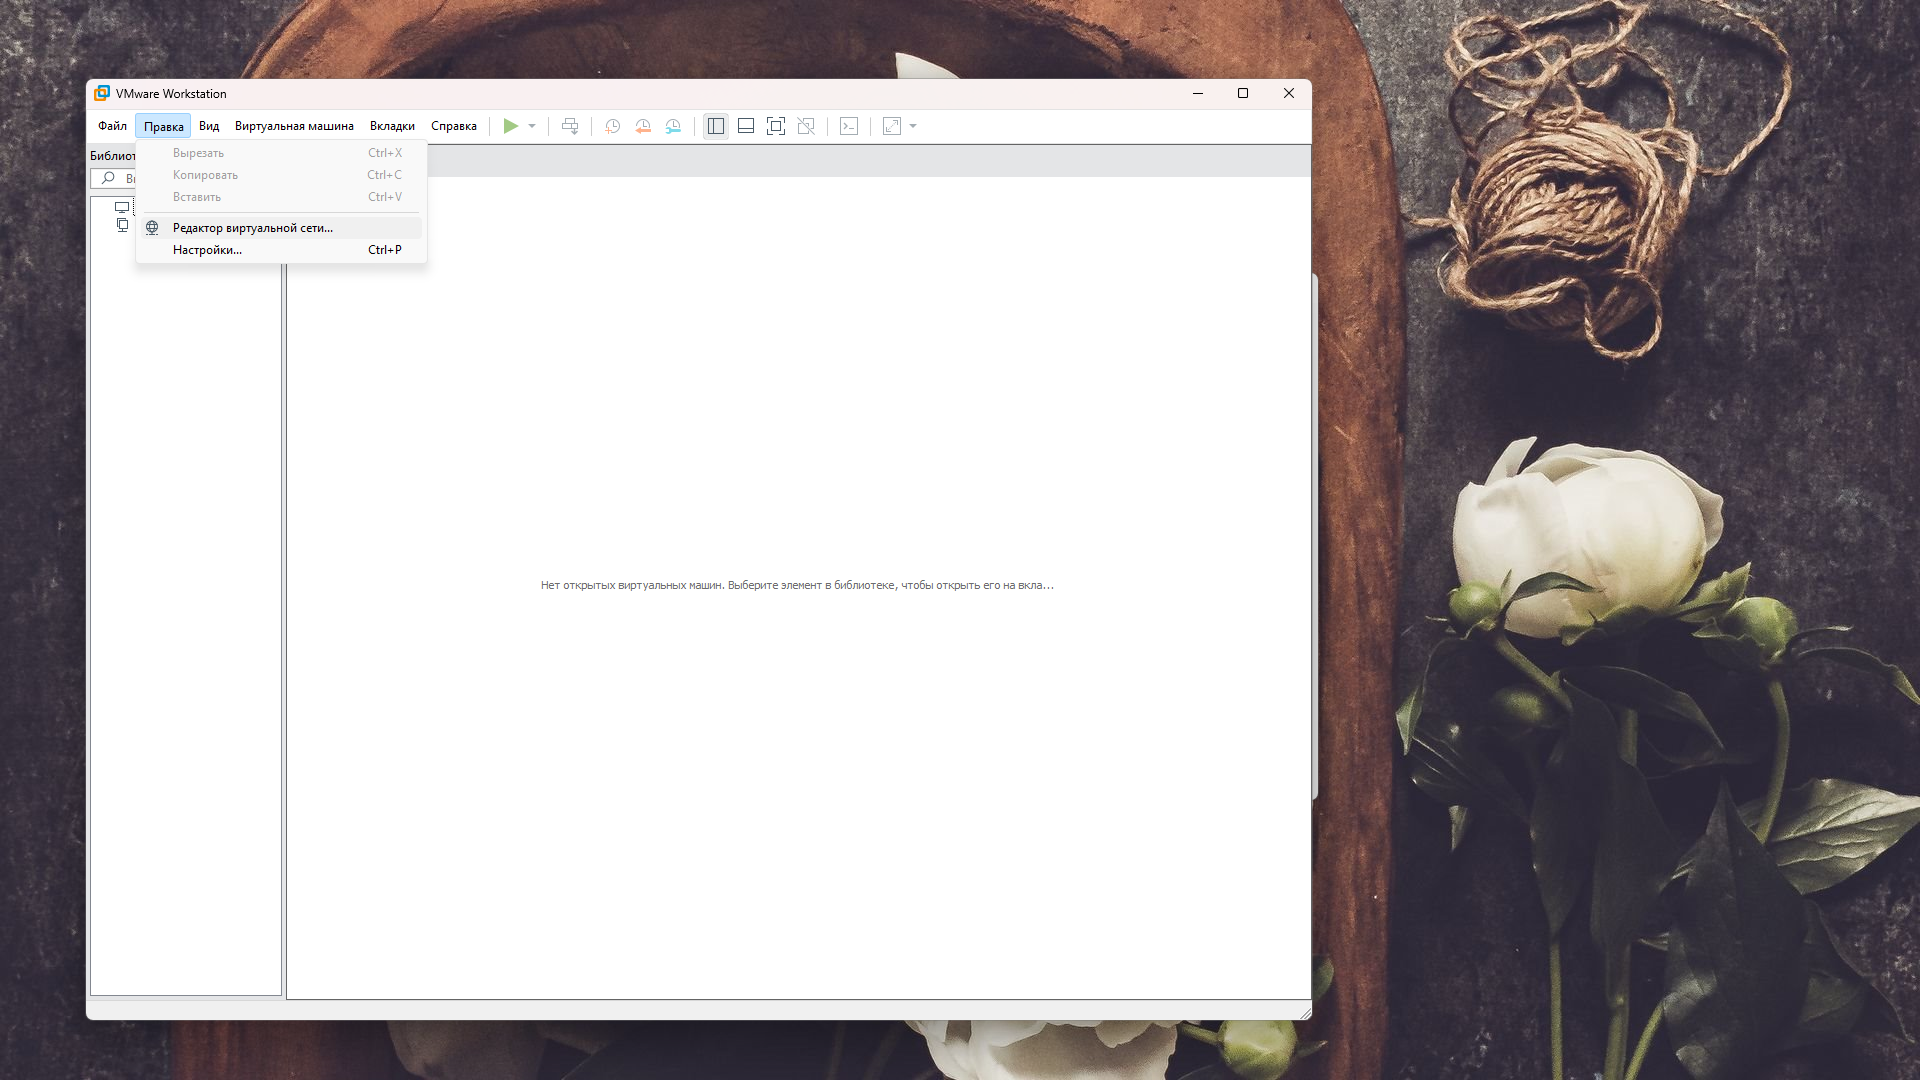
\includegraphics[width=0.85\textwidth]{06_00 (2)}
    \label{img:2}
    \caption{Открываем редактор виртульной сети}
  \end{figure}
  
  \begin{figure}[H]
    \centering
    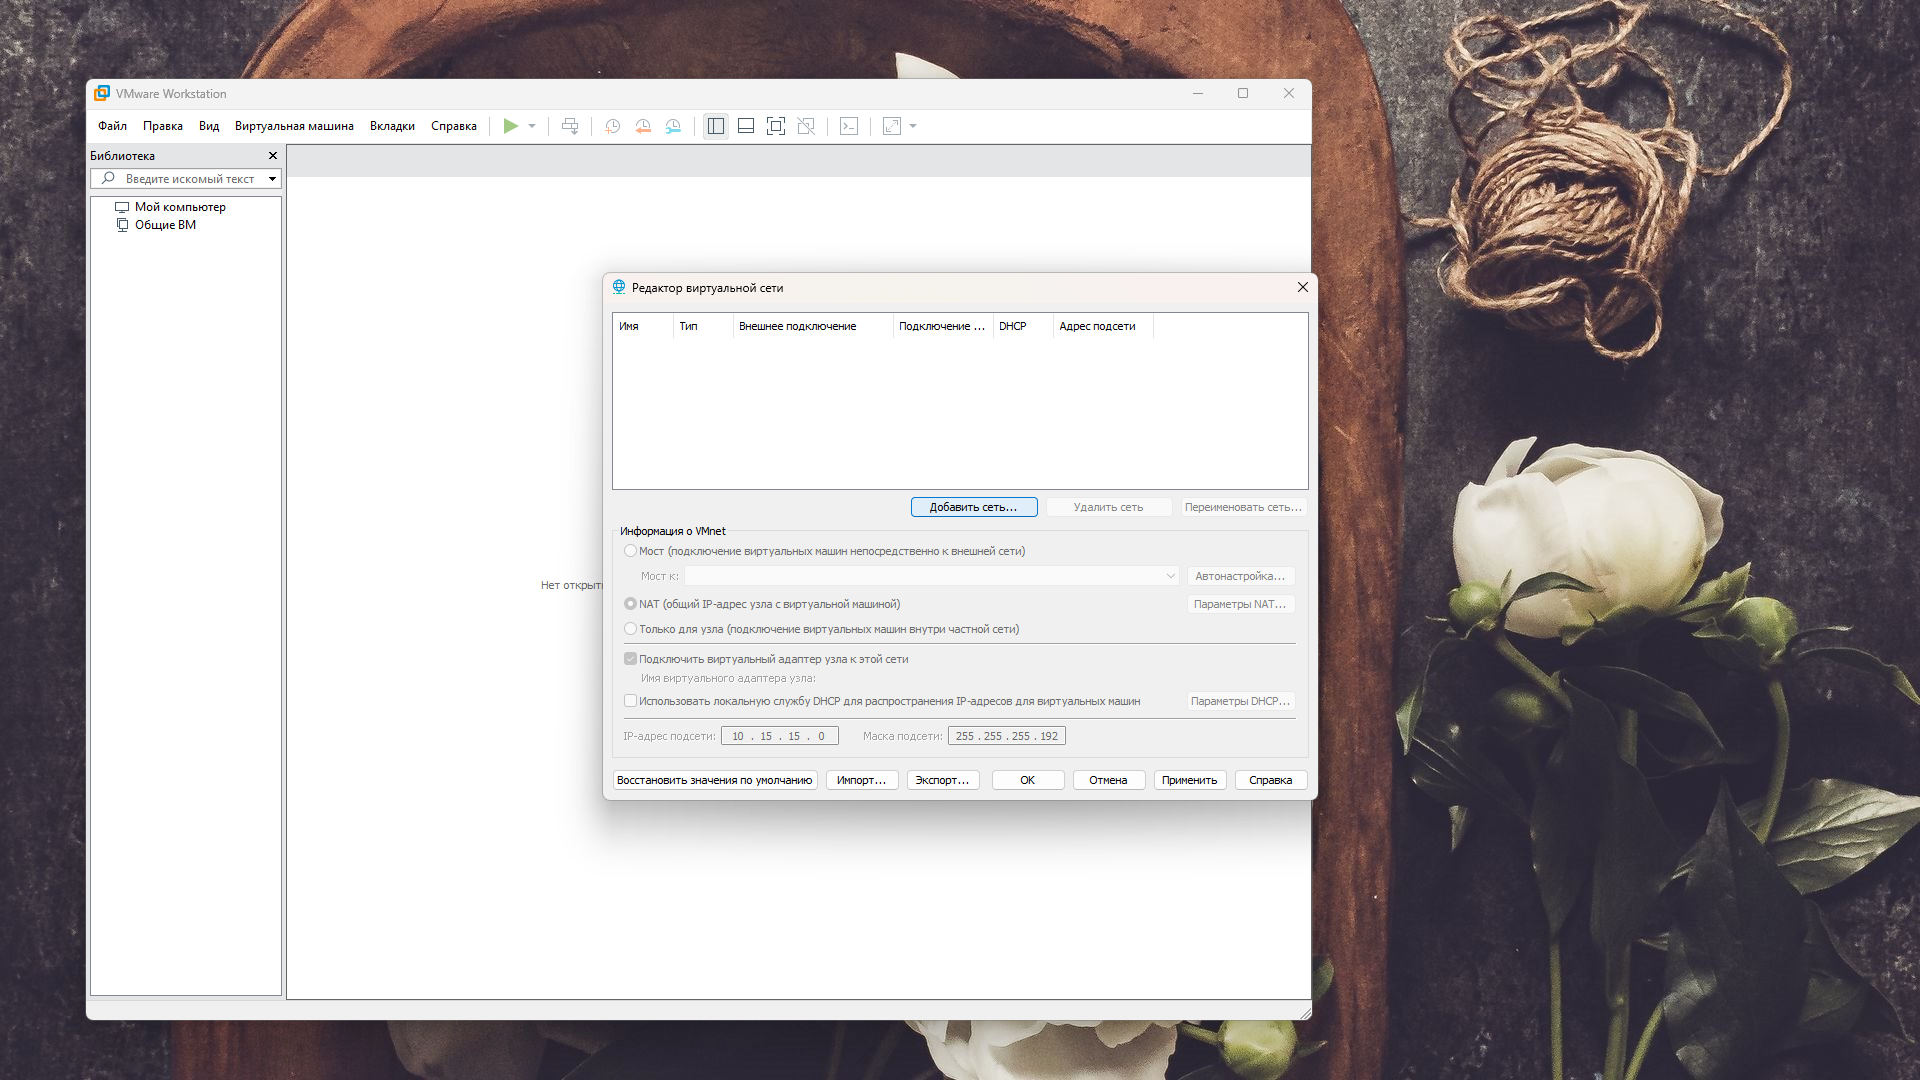
\includegraphics[width=0.85\textwidth]{06_00 (3)}
    \label{img:3}
    \caption{Добавляем новую сеть}
  \end{figure}
  
  \begin{figure}[H]
    \centering
    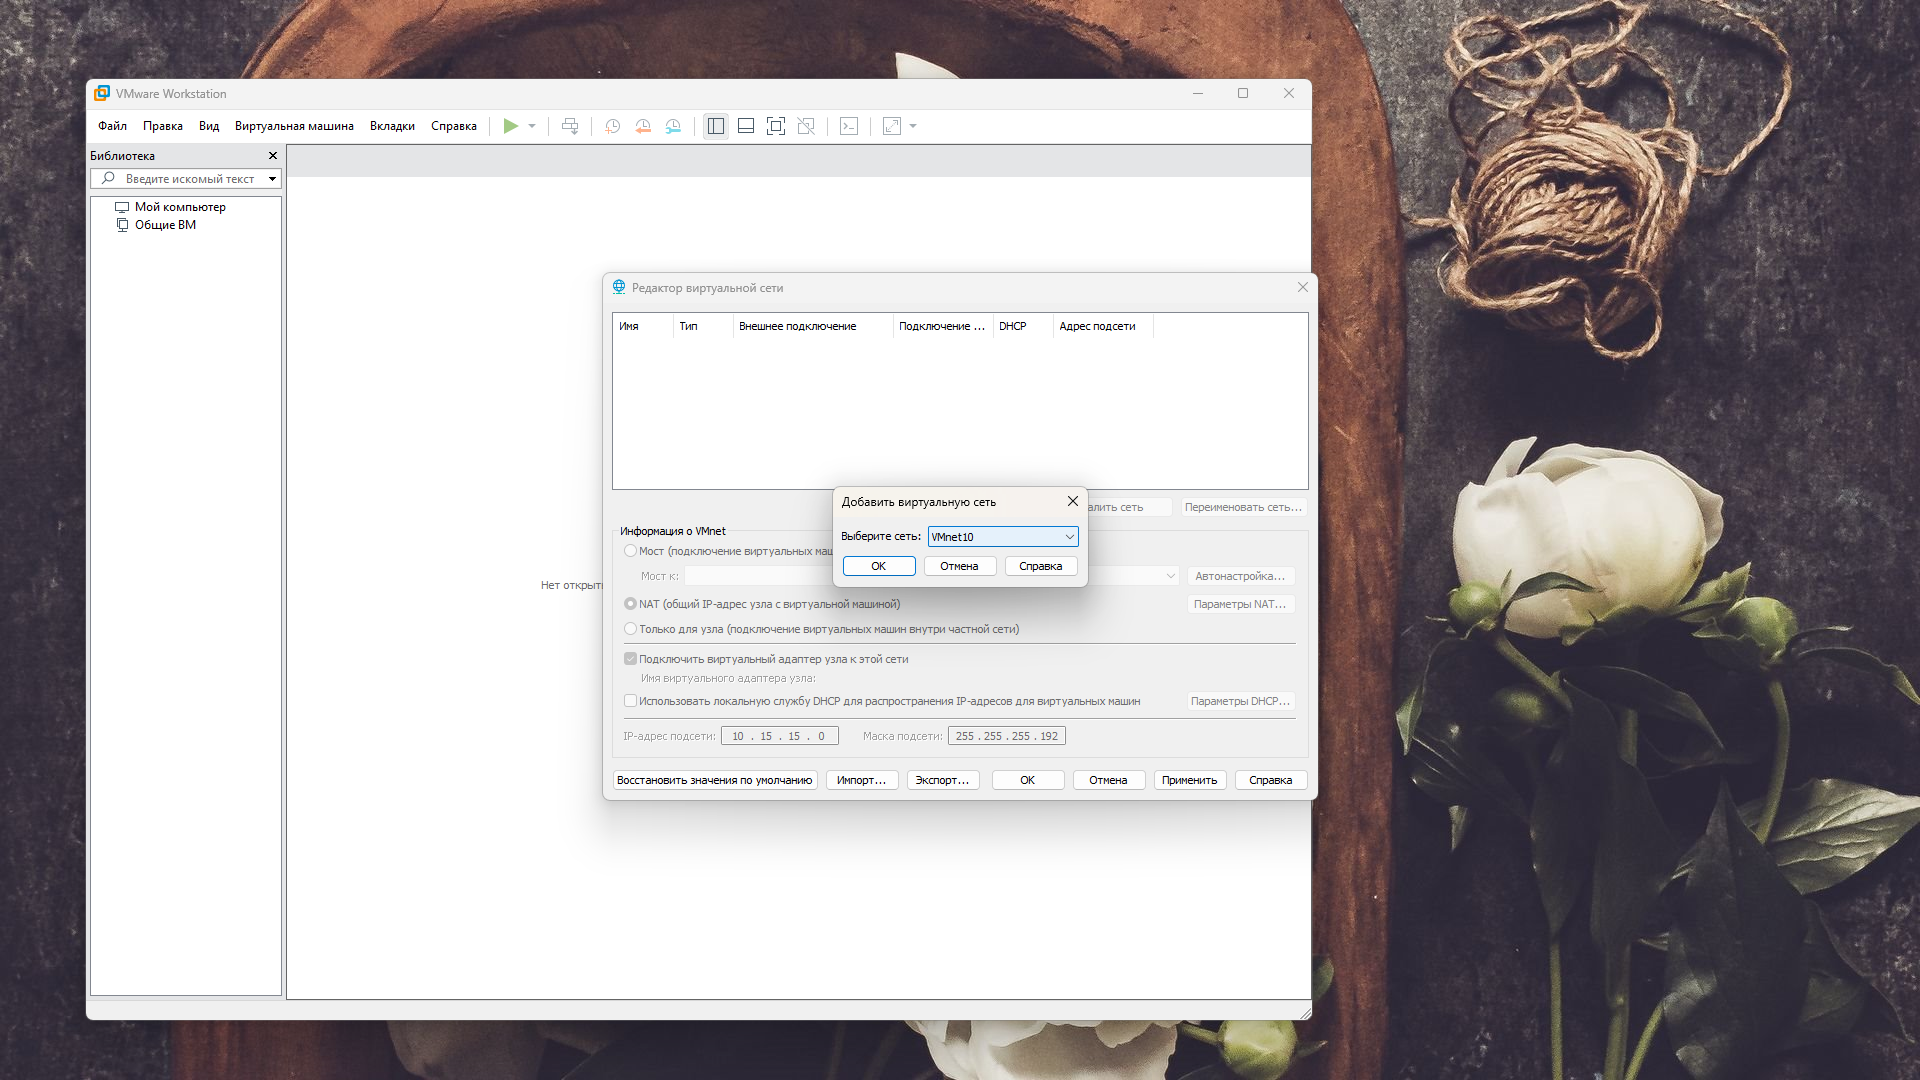
\includegraphics[width=0.85\textwidth]{06_00 (4)}
    \label{img:4}
    \caption{Выбираем ее имя, в моем случае - VMNet10}
  \end{figure}
  
  Далее необходимо указать параметры новой сети: включить \textit{NAT},
  чтобы задать тип этой сети, подключить к ней виртуальный адаптер (чтобы хостовая машина,
  на которой запускаются виртуальные, тоже имела к ней доступ), включить \textit{DHCP},
  а также указать параметры.

  Для 9-ого варианта параметры сети указаны следующие:
  \begin{table}[H]
    \centering
    \begin{tabular}{|c|c|}
      \hline
      Адрес сети & 10.15.10.0/26 \\
      \hline
      Шлюз & 10.15.10.10 \\
      \hline
      DNS & 10.15.10.10 \\
      \hline      
    \end{tabular}
  \end{table}

  \begin{figure}[H]
    \centering
    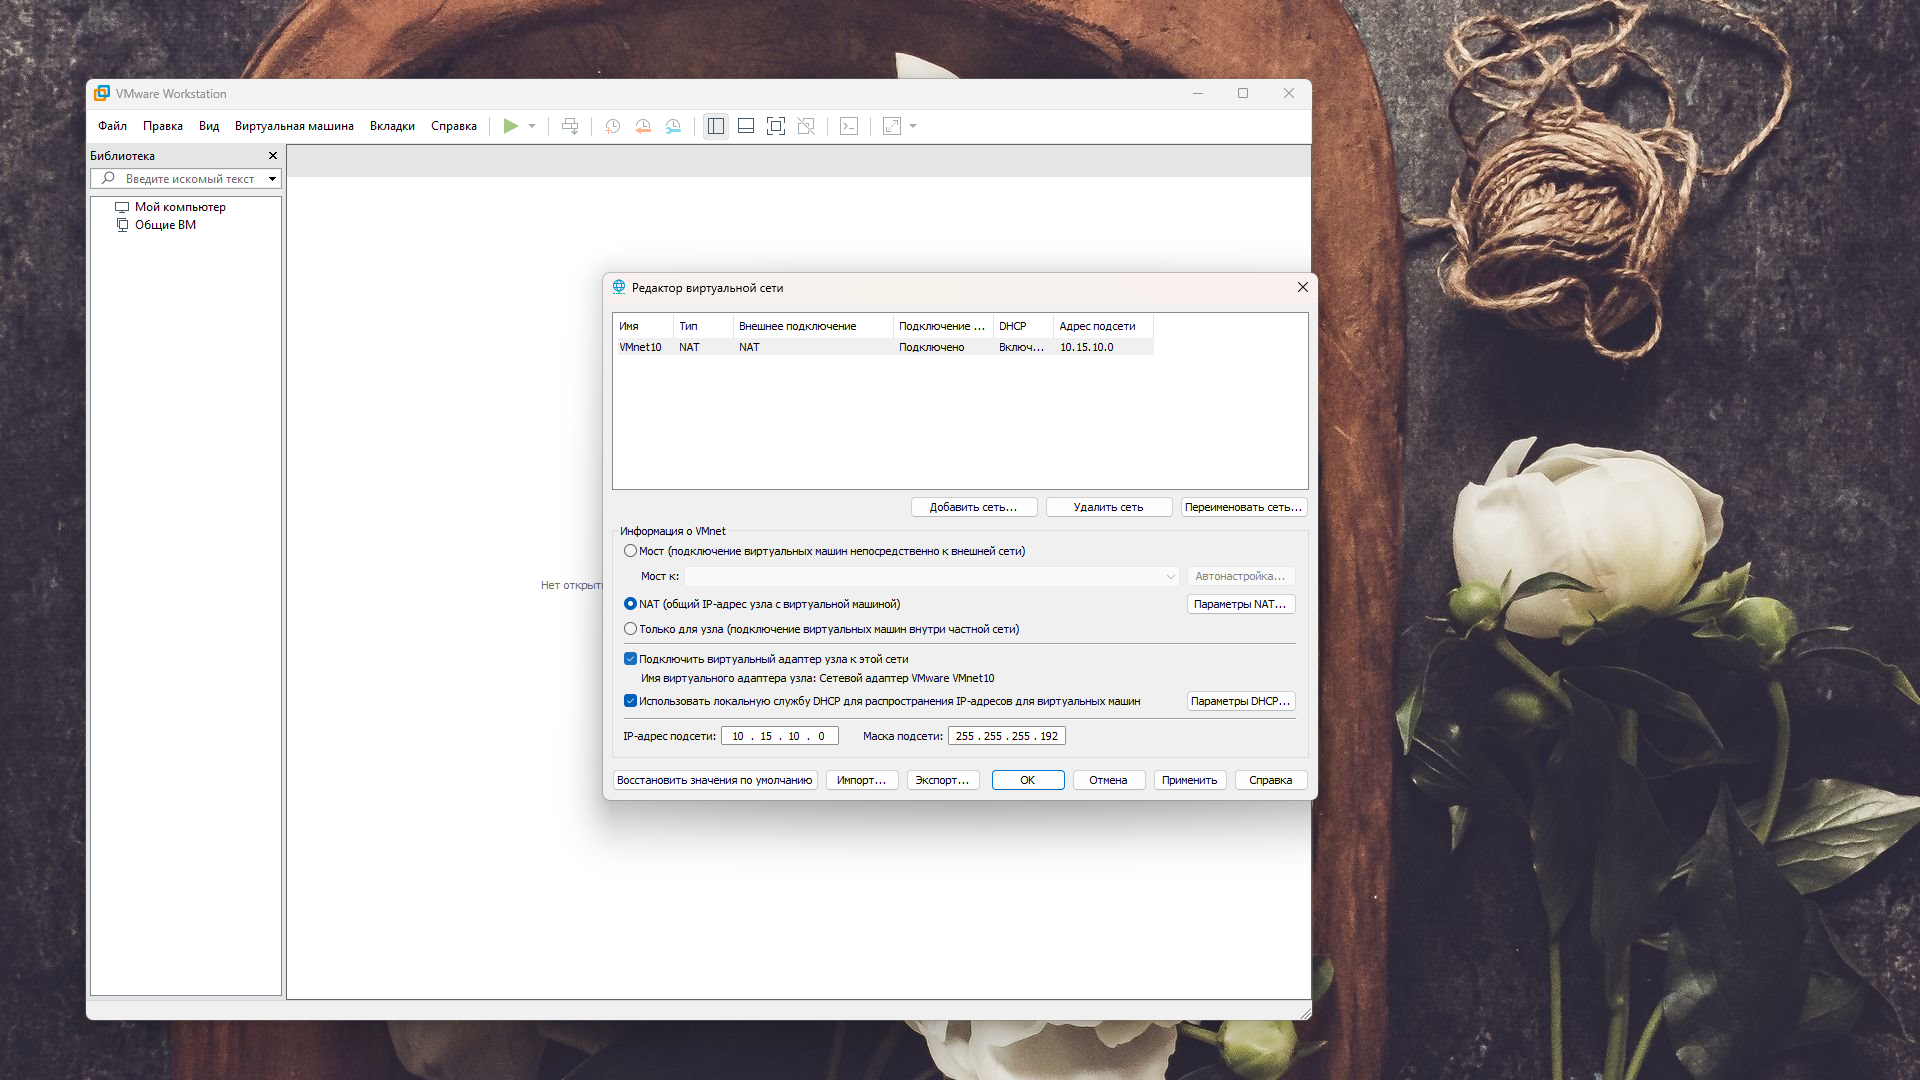
\includegraphics[width=0.85\textwidth]{06_00 (5)}
    \label{img:5}
    \caption{Указываем адрес подсети и маску}
  \end{figure}
  
  \begin{figure}[H]
    \centering
    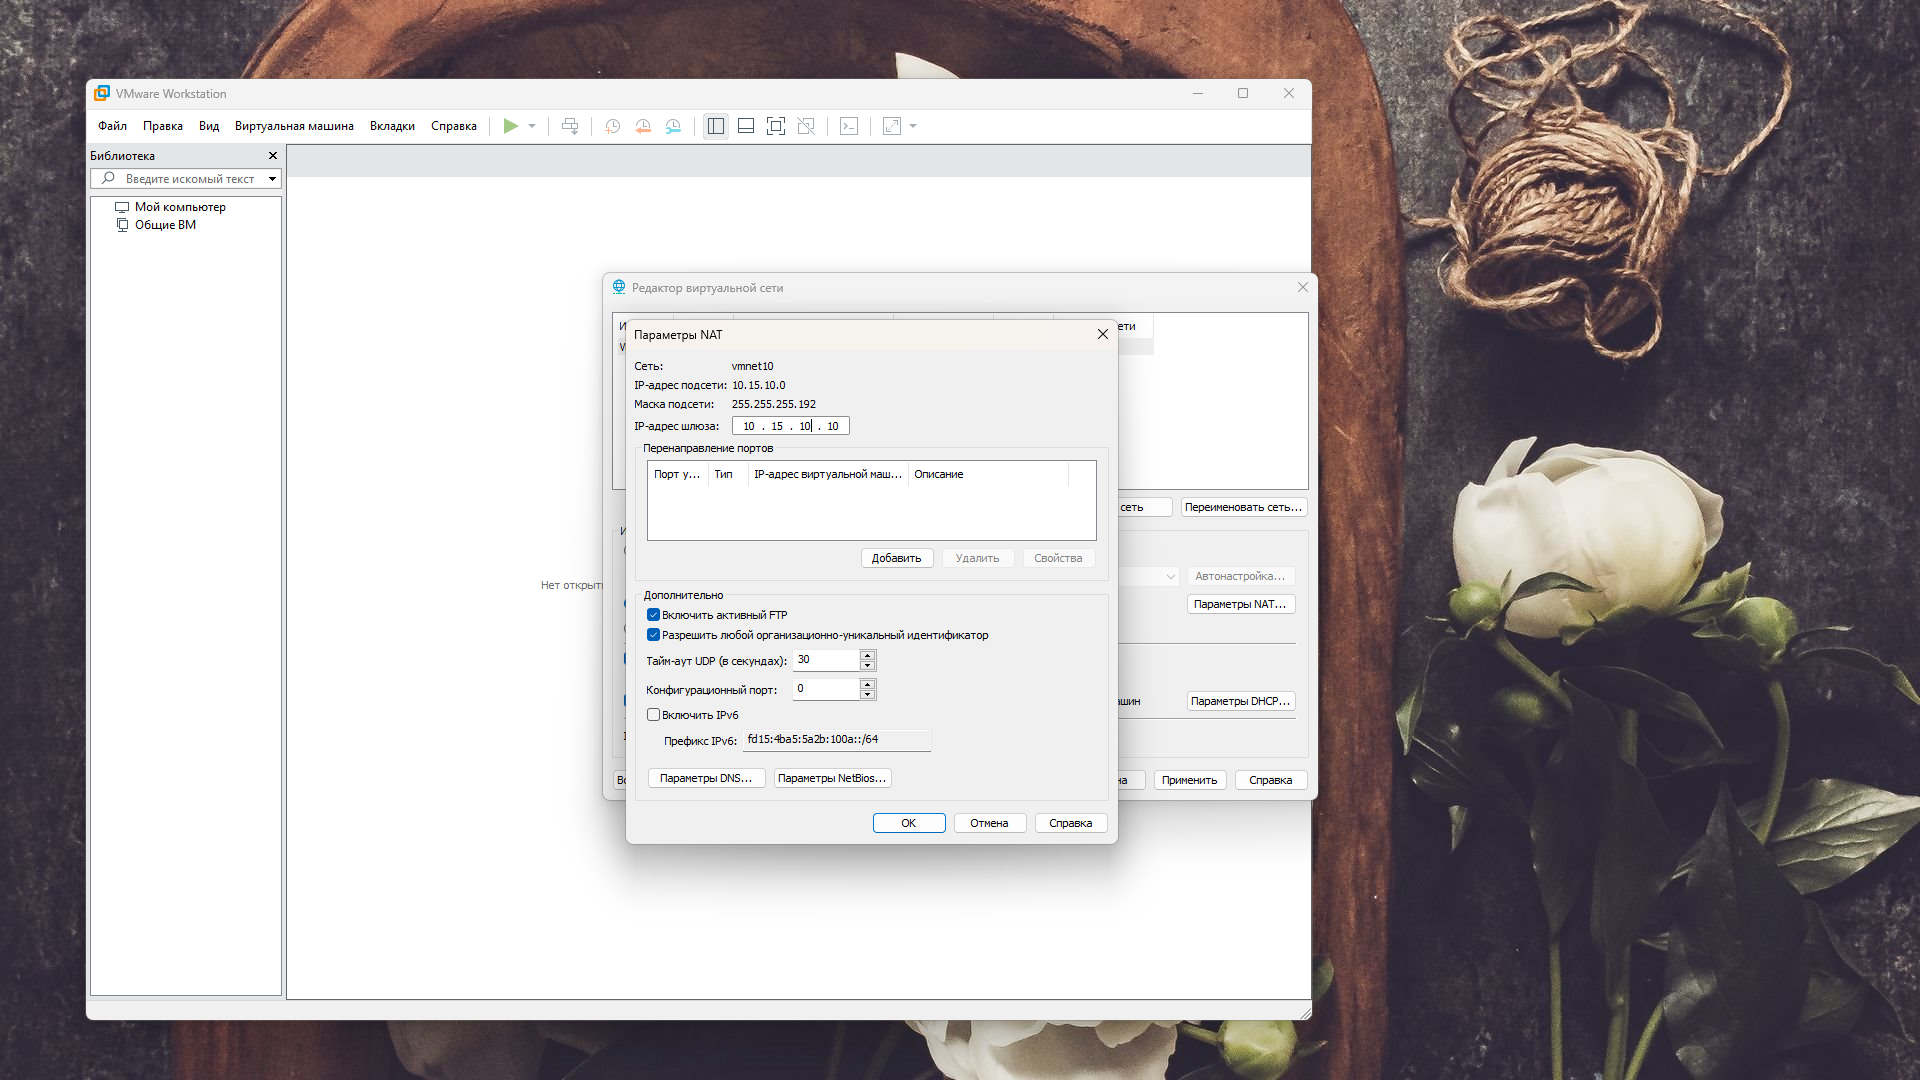
\includegraphics[width=0.85\textwidth]{06_00 (6)}
    \label{img:6}
    \caption{Для настройки шлюза открываем параметры NAT и указываем нужый адрес там}
  \end{figure}

  На данном этапе эту сеть можно считать настроенной.

  \subsubsection{Создание ВМ с Windows 10}  

  Был заранее скачан готовый образ - откроем его:

  \begin{figure}[H]
    \centering
    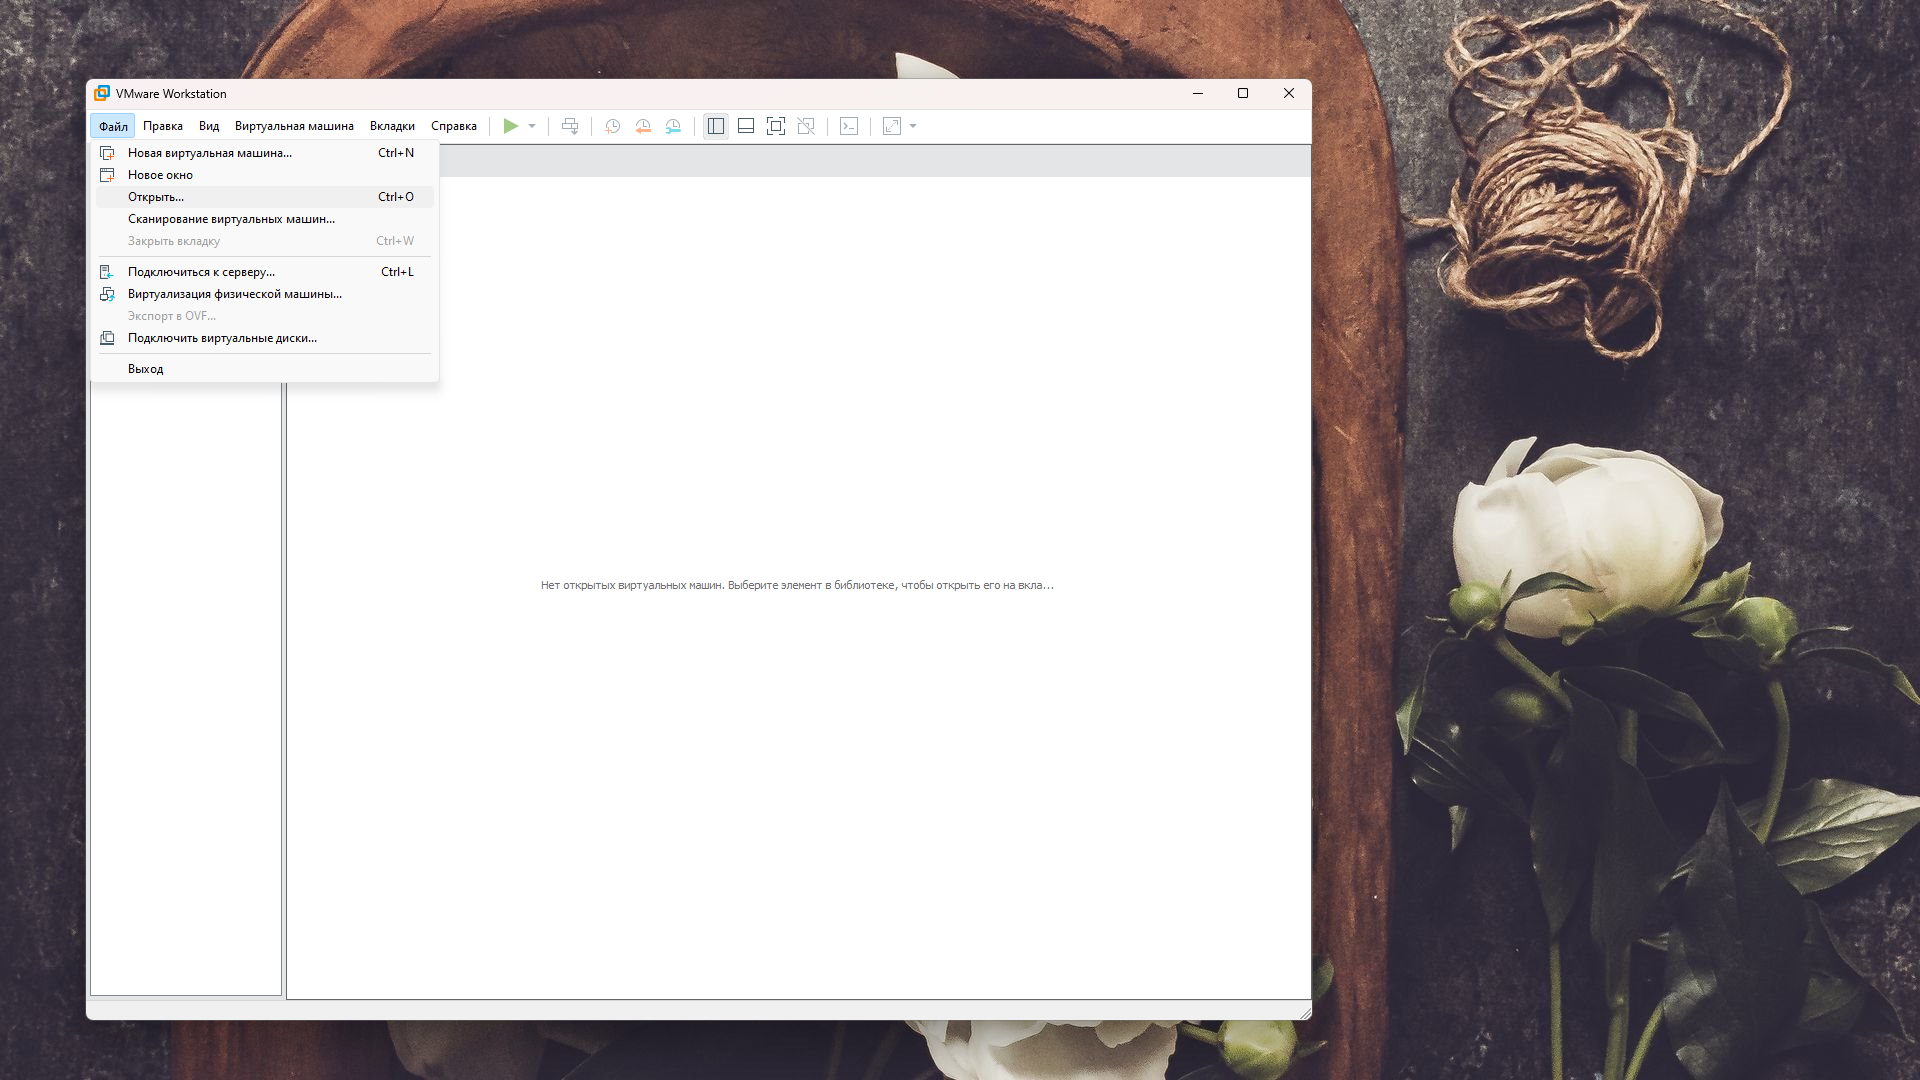
\includegraphics[width=0.85\textwidth]{06_00 (7)}
    \label{img:7}
    \caption{Выбираем пункт "Открыть" в меню}
  \end{figure}
  
  \begin{figure}[H]
    \centering
    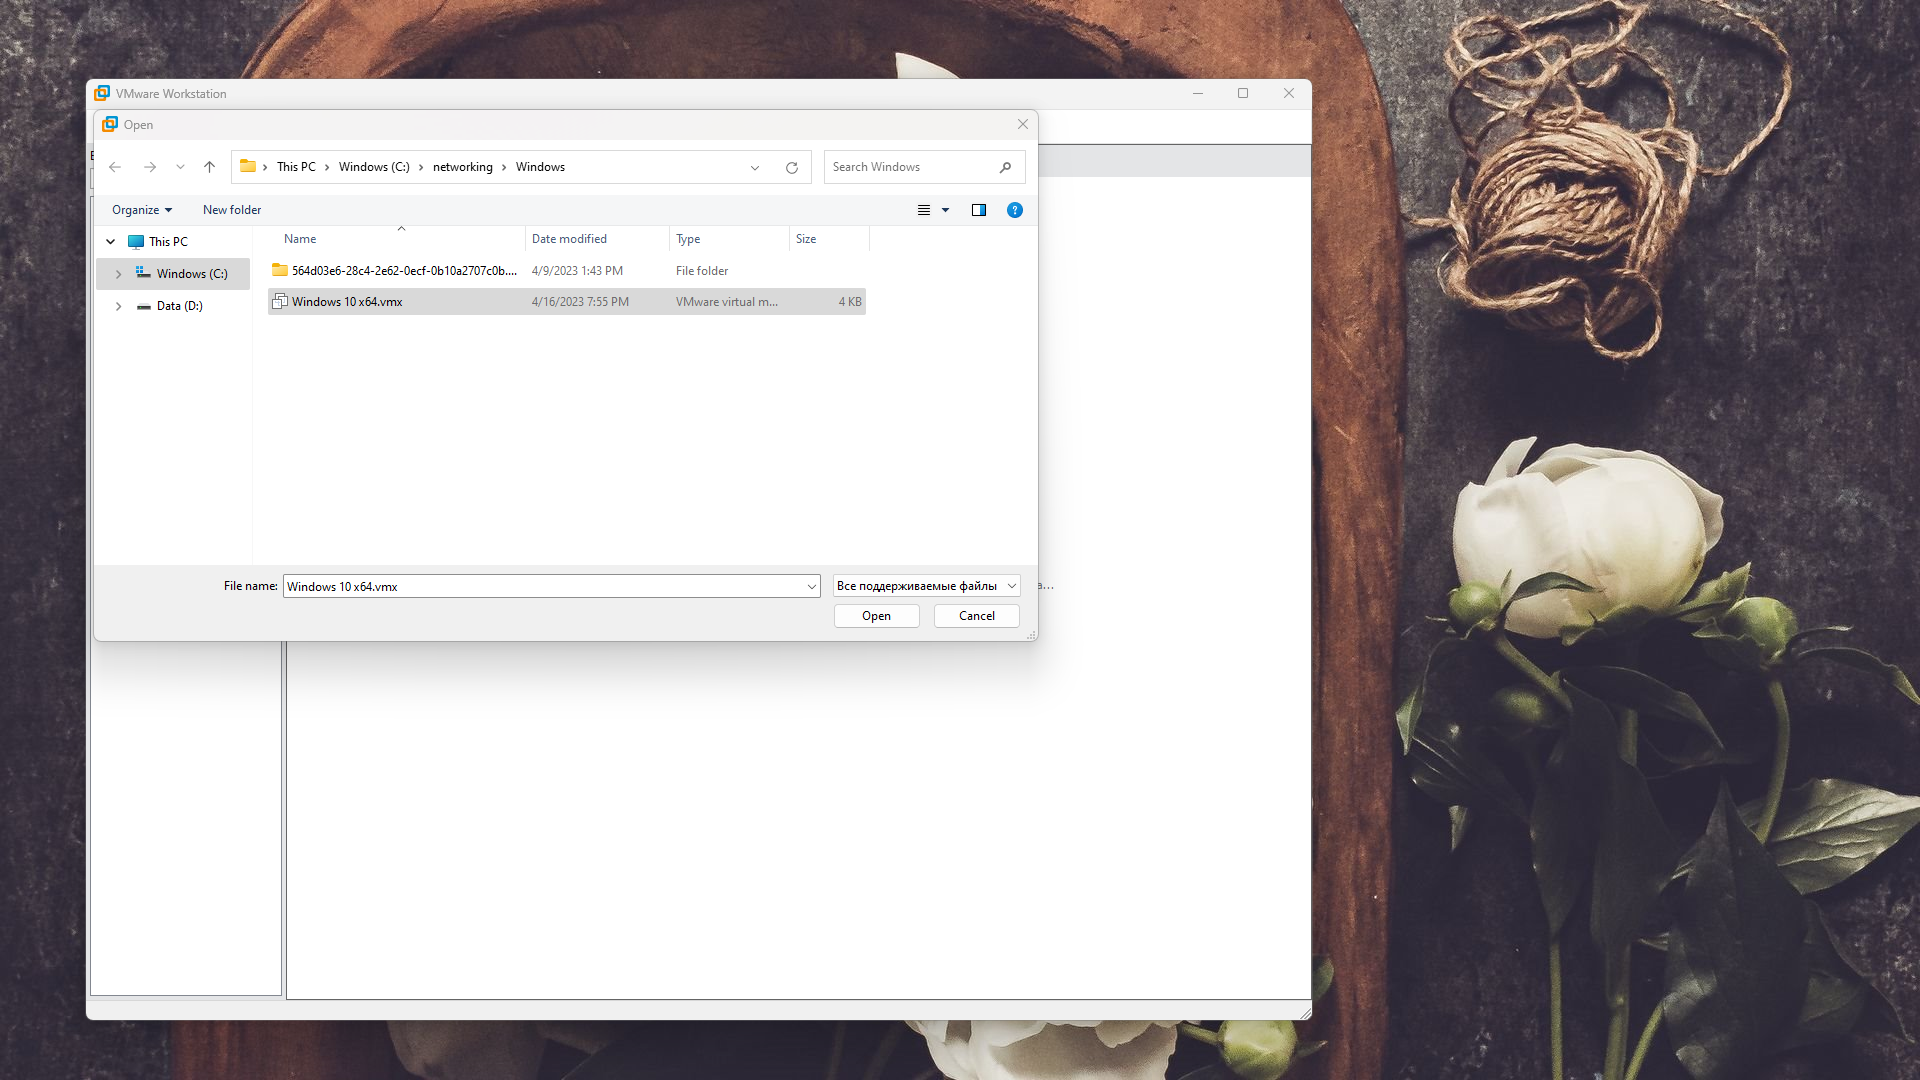
\includegraphics[width=0.85\textwidth]{06_00 (8)}
    \label{img:8}
    \caption{Указываем путь до необходимого образа}
  \end{figure}
  
  \begin{figure}[H]
    \centering
    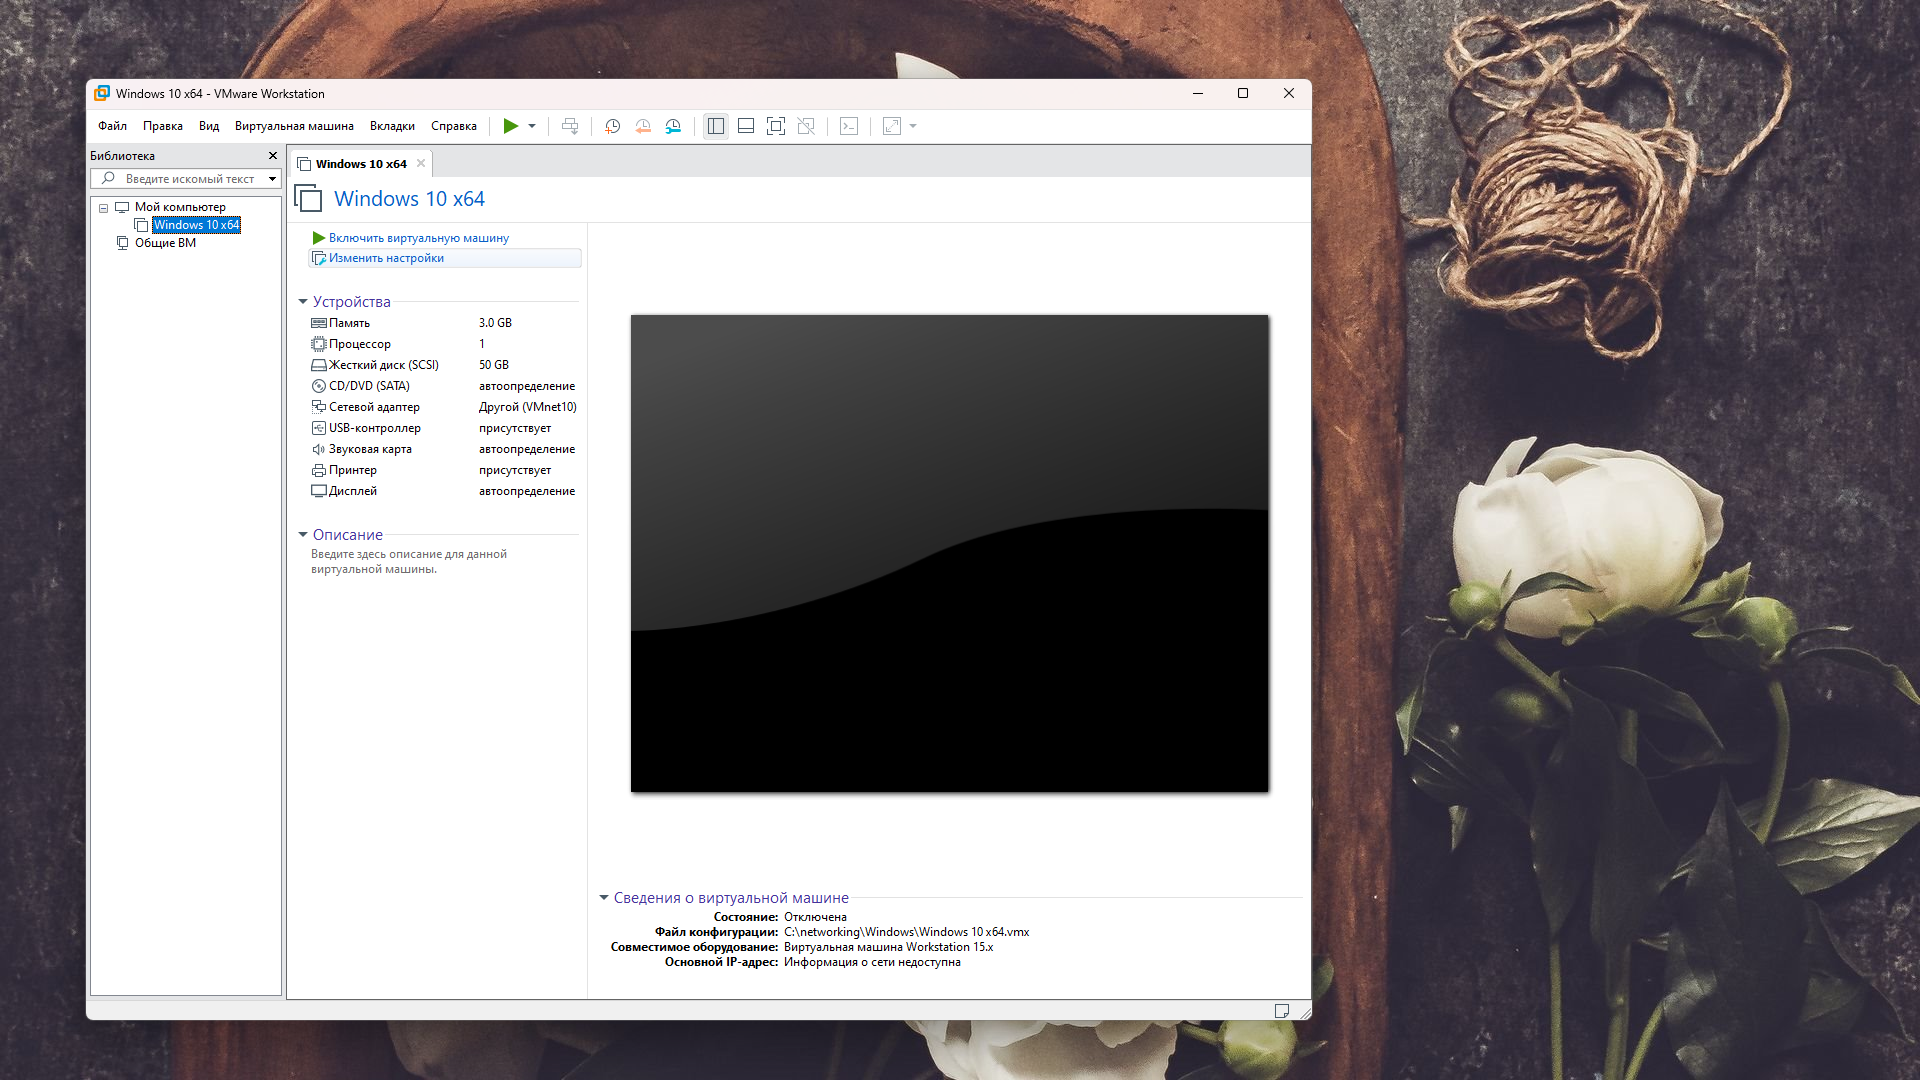
\includegraphics[width=0.85\textwidth]{06_00 (9)}
    \label{img:9}
    \caption{Виртуальная машина импортирована}
  \end{figure}
  
  \begin{figure}[H]
    \centering
    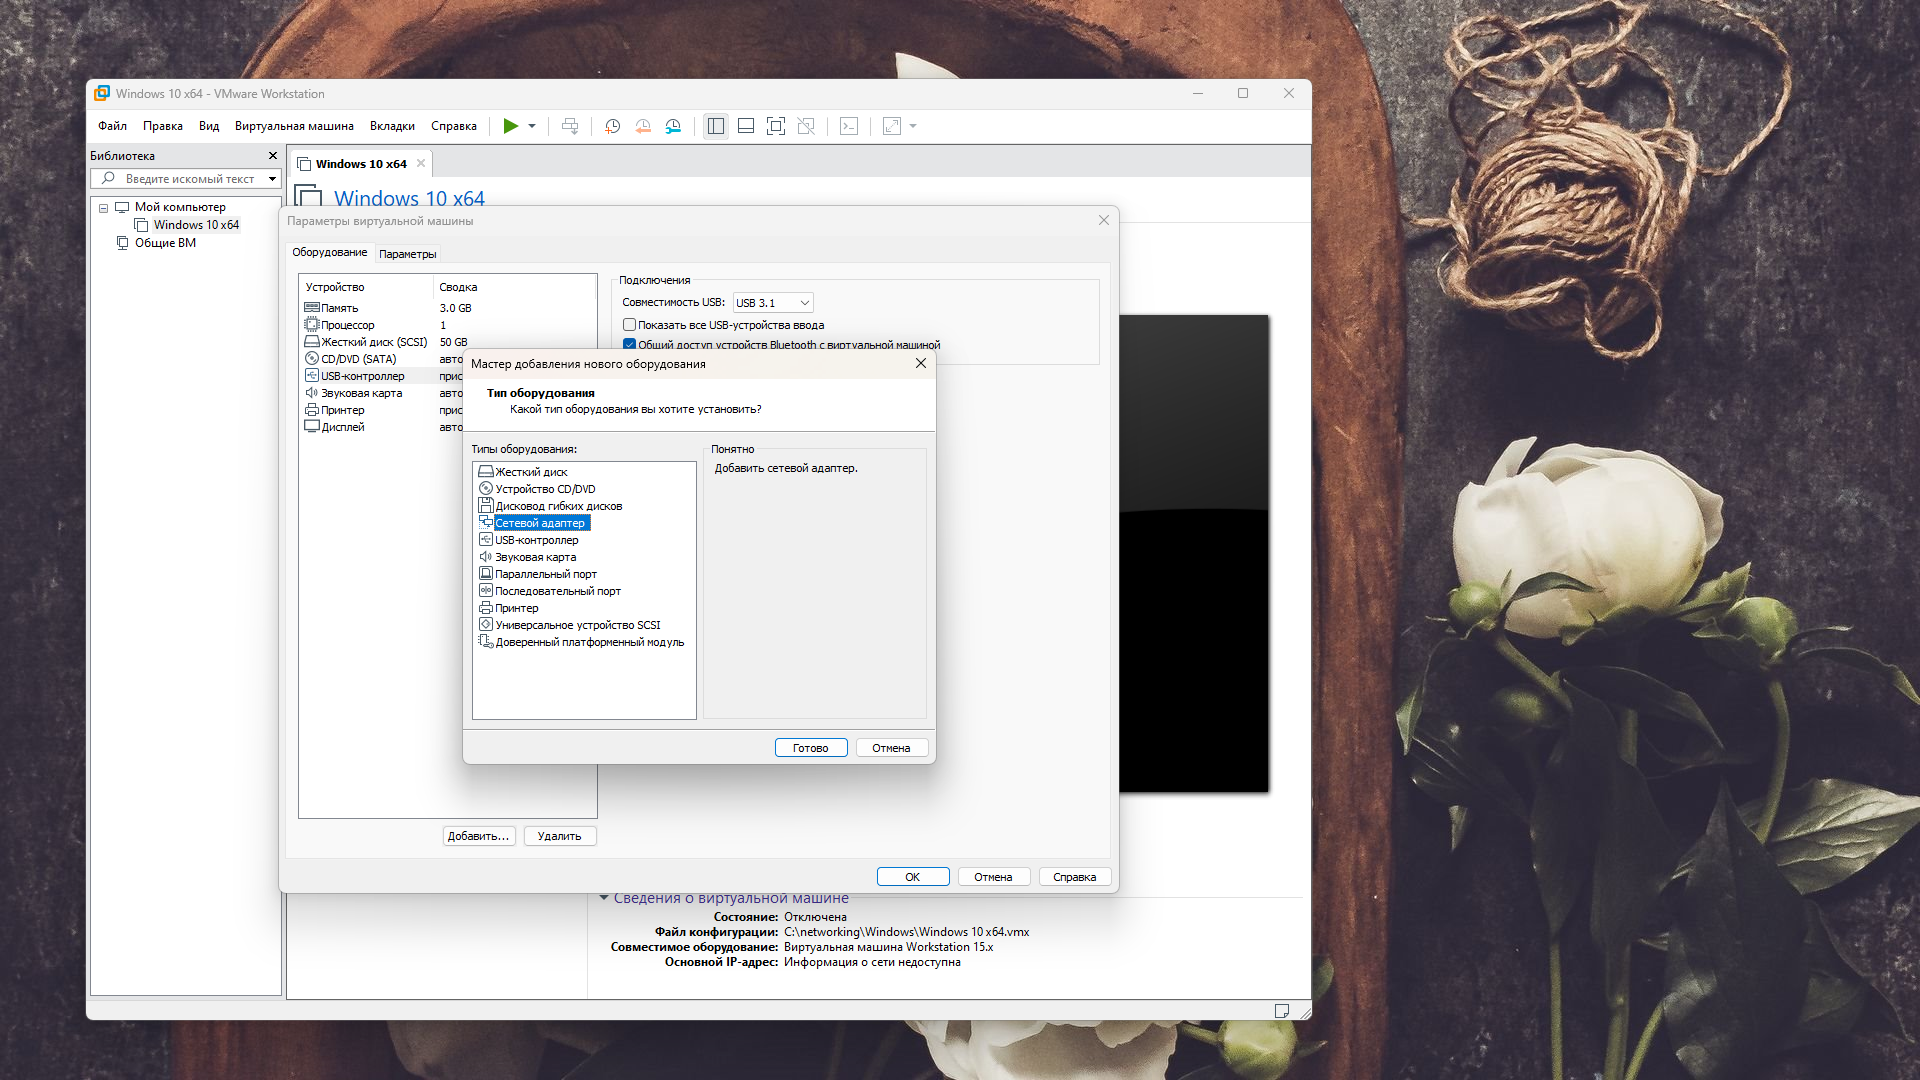
\includegraphics[width=0.85\textwidth]{06_00 (10)}
    \label{img:10}
    \caption{Откроем настройки только что созданной машины и создадим для нее новый сетевой адаптер}
  \end{figure}
  
  \begin{figure}[H]
    \centering
    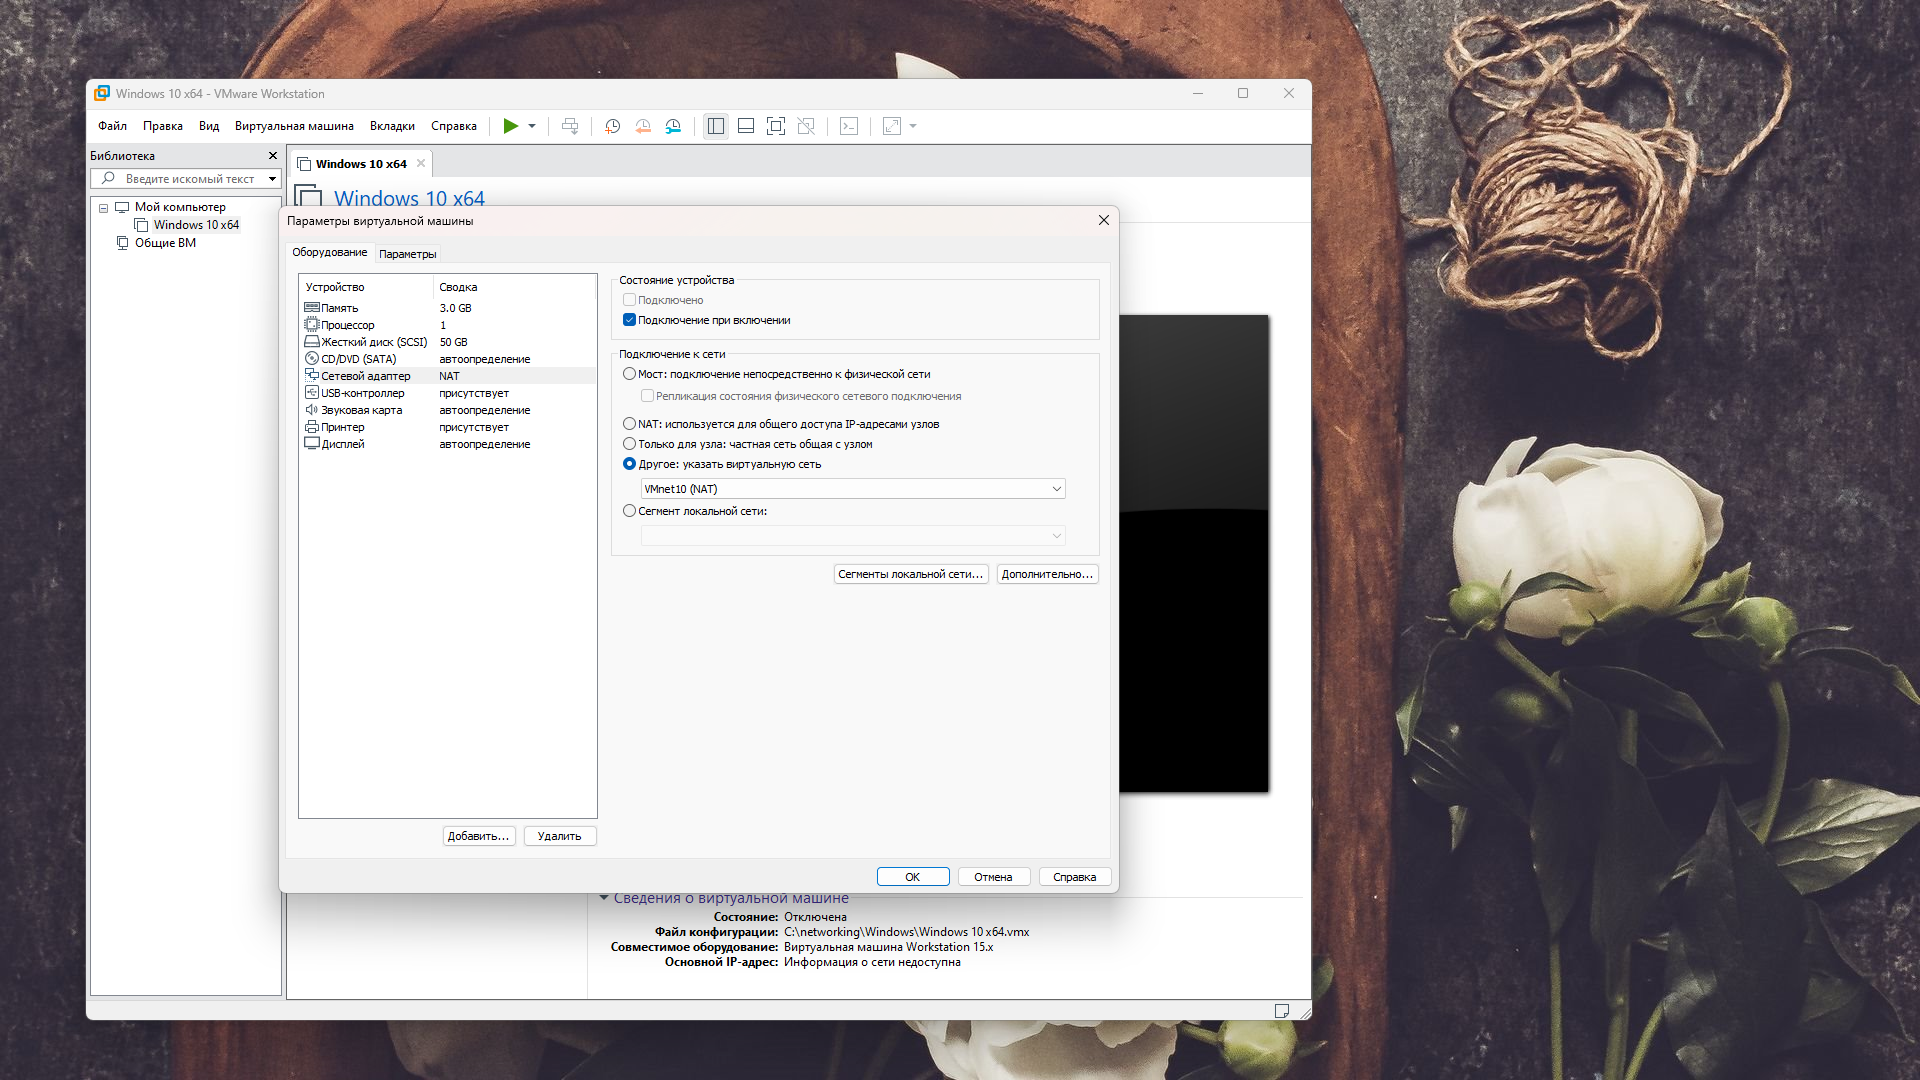
\includegraphics[width=0.85\textwidth]{06_00 (11)}
    \label{img:11}
    \caption{Подключим его к ранее настроенной NAT сети}
  \end{figure}
  
  \begin{figure}[H]
    \centering
    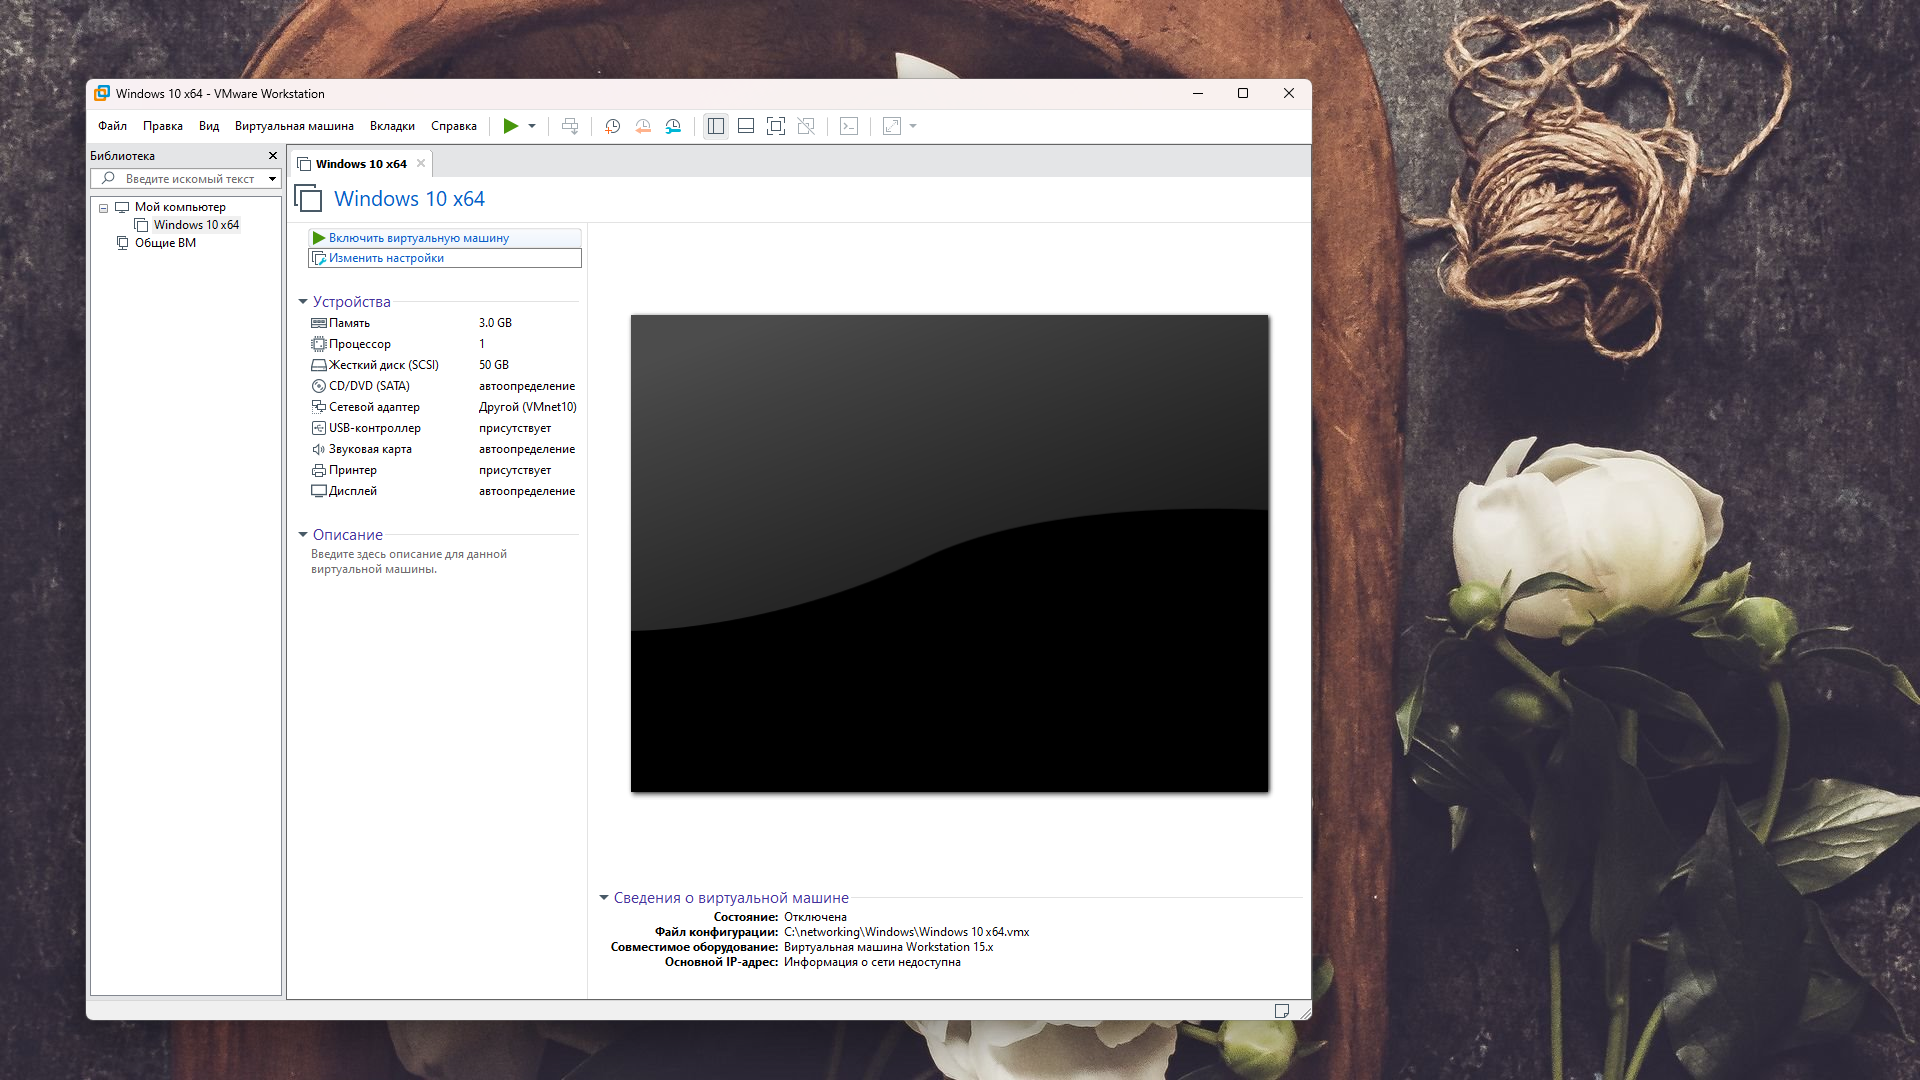
\includegraphics[width=0.85\textwidth]{06_00 (12)}
    \label{img:12}
    \caption{Теперь машина готова к работе}
  \end{figure}
  
  \subsubsection{Динамическое получение адреса в Windows 10}

  \begin{figure}[H]
    \centering
    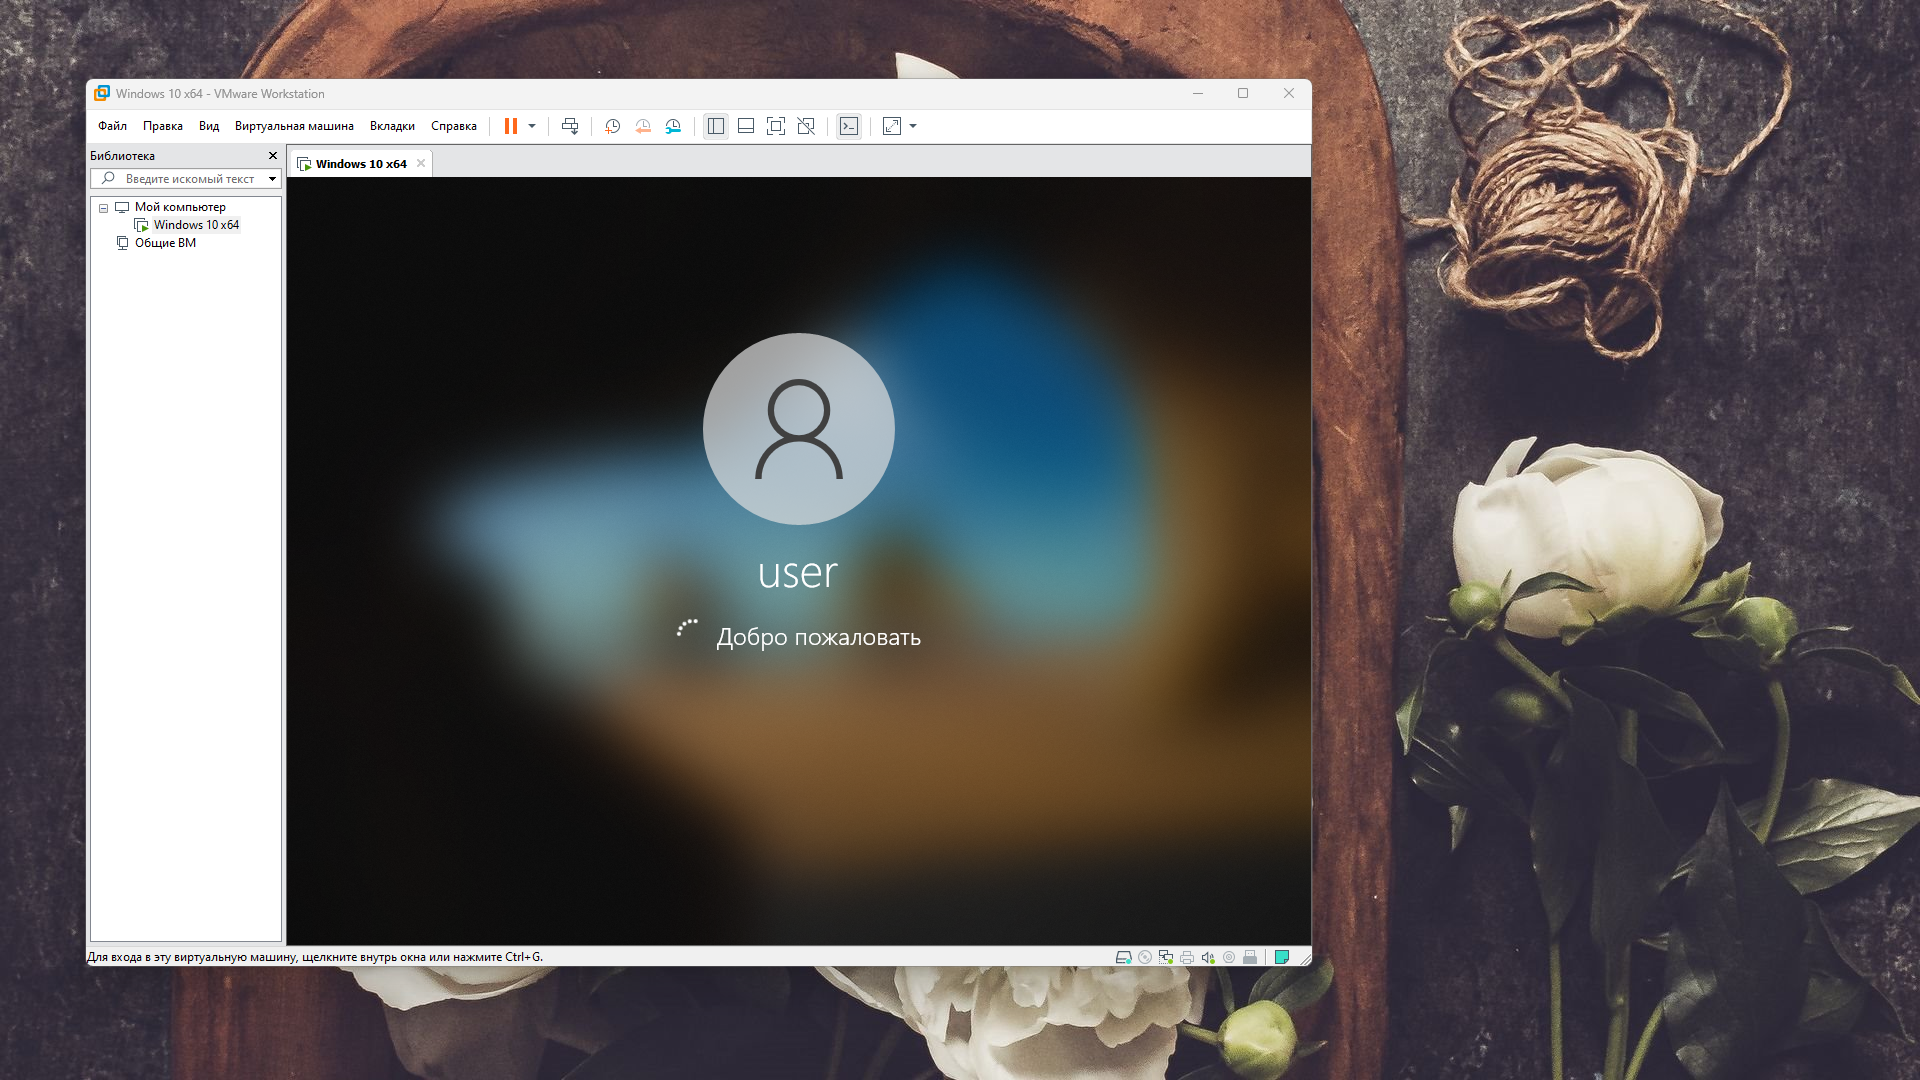
\includegraphics[width=0.85\textwidth]{06_00 (13)}
    \label{img:13}
    \caption{Входим в учетную запись пользователя}
  \end{figure}
  
  \begin{figure}[H]
    \centering
    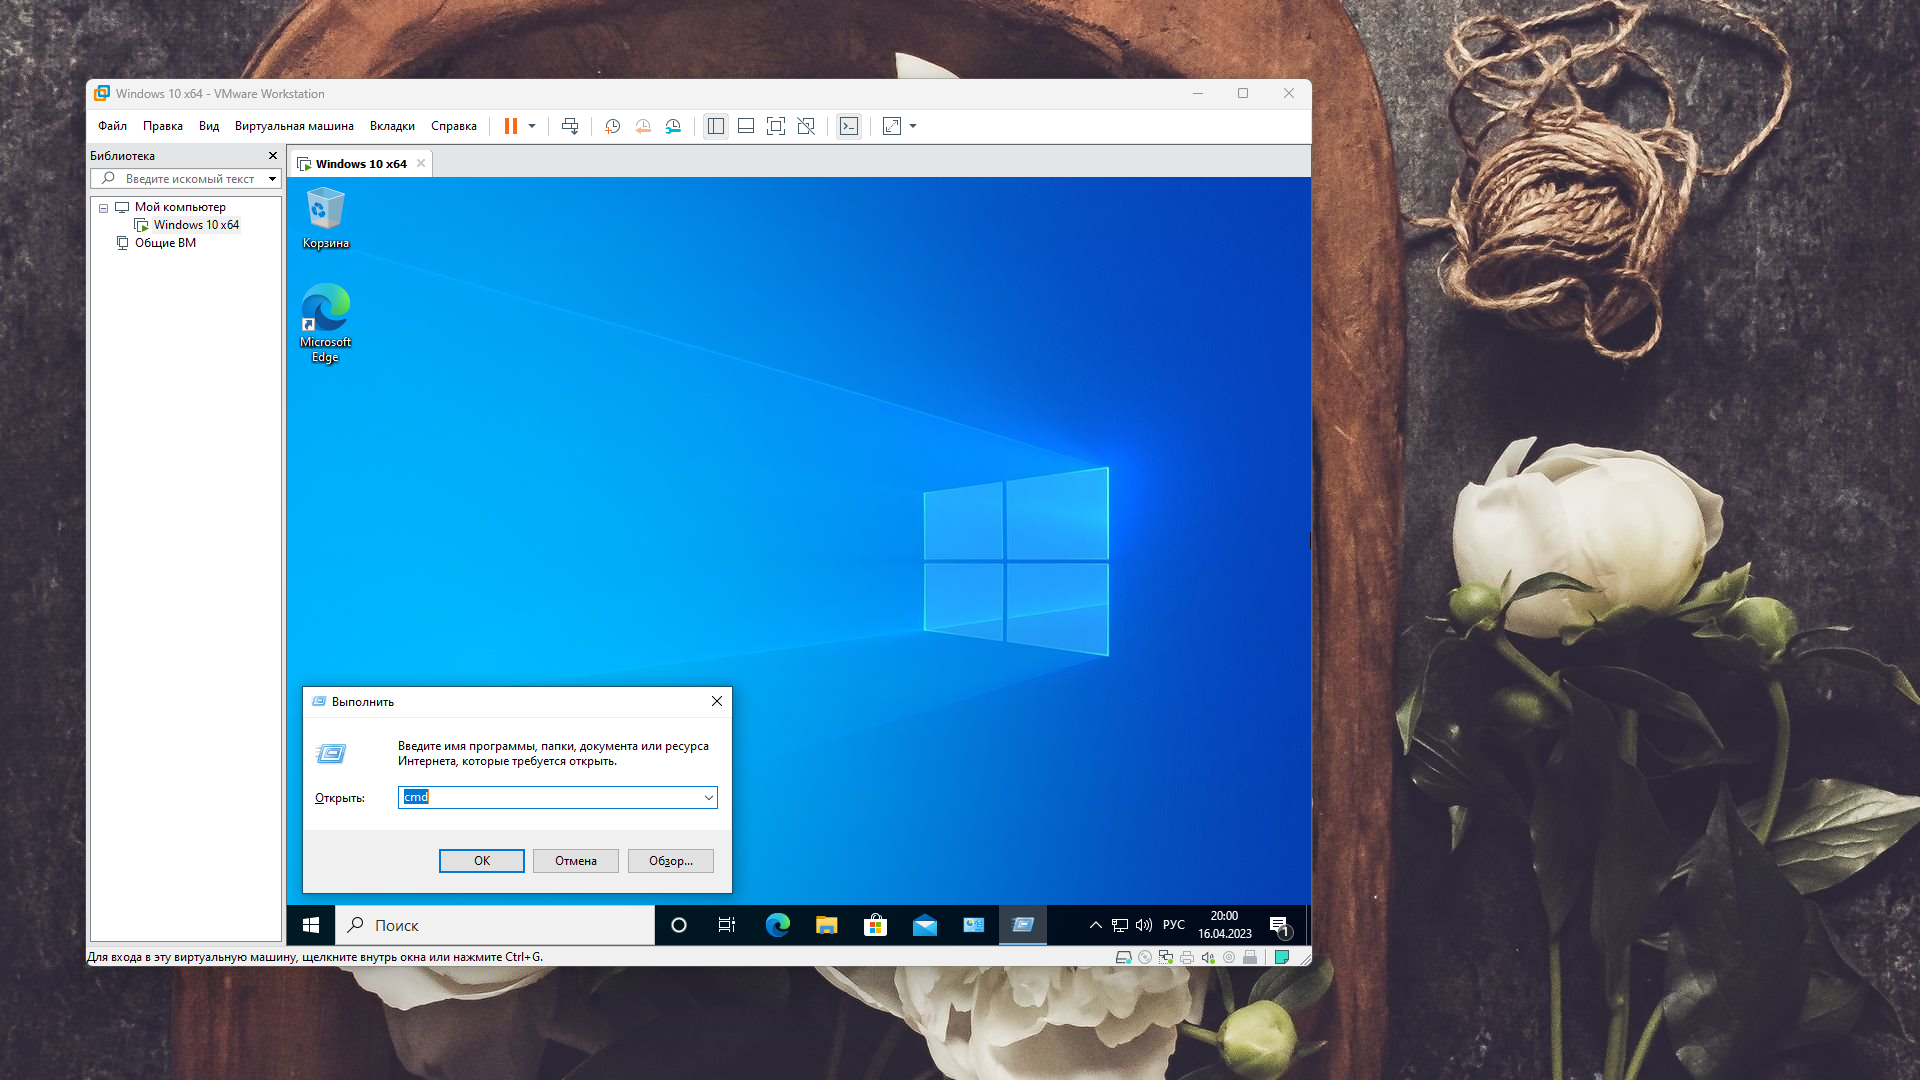
\includegraphics[width=0.85\textwidth]{06_00 (14)}
    \label{img:14}
    \caption{Открываем камандную строку}
  \end{figure}
  
  \begin{figure}[H]
    \centering
    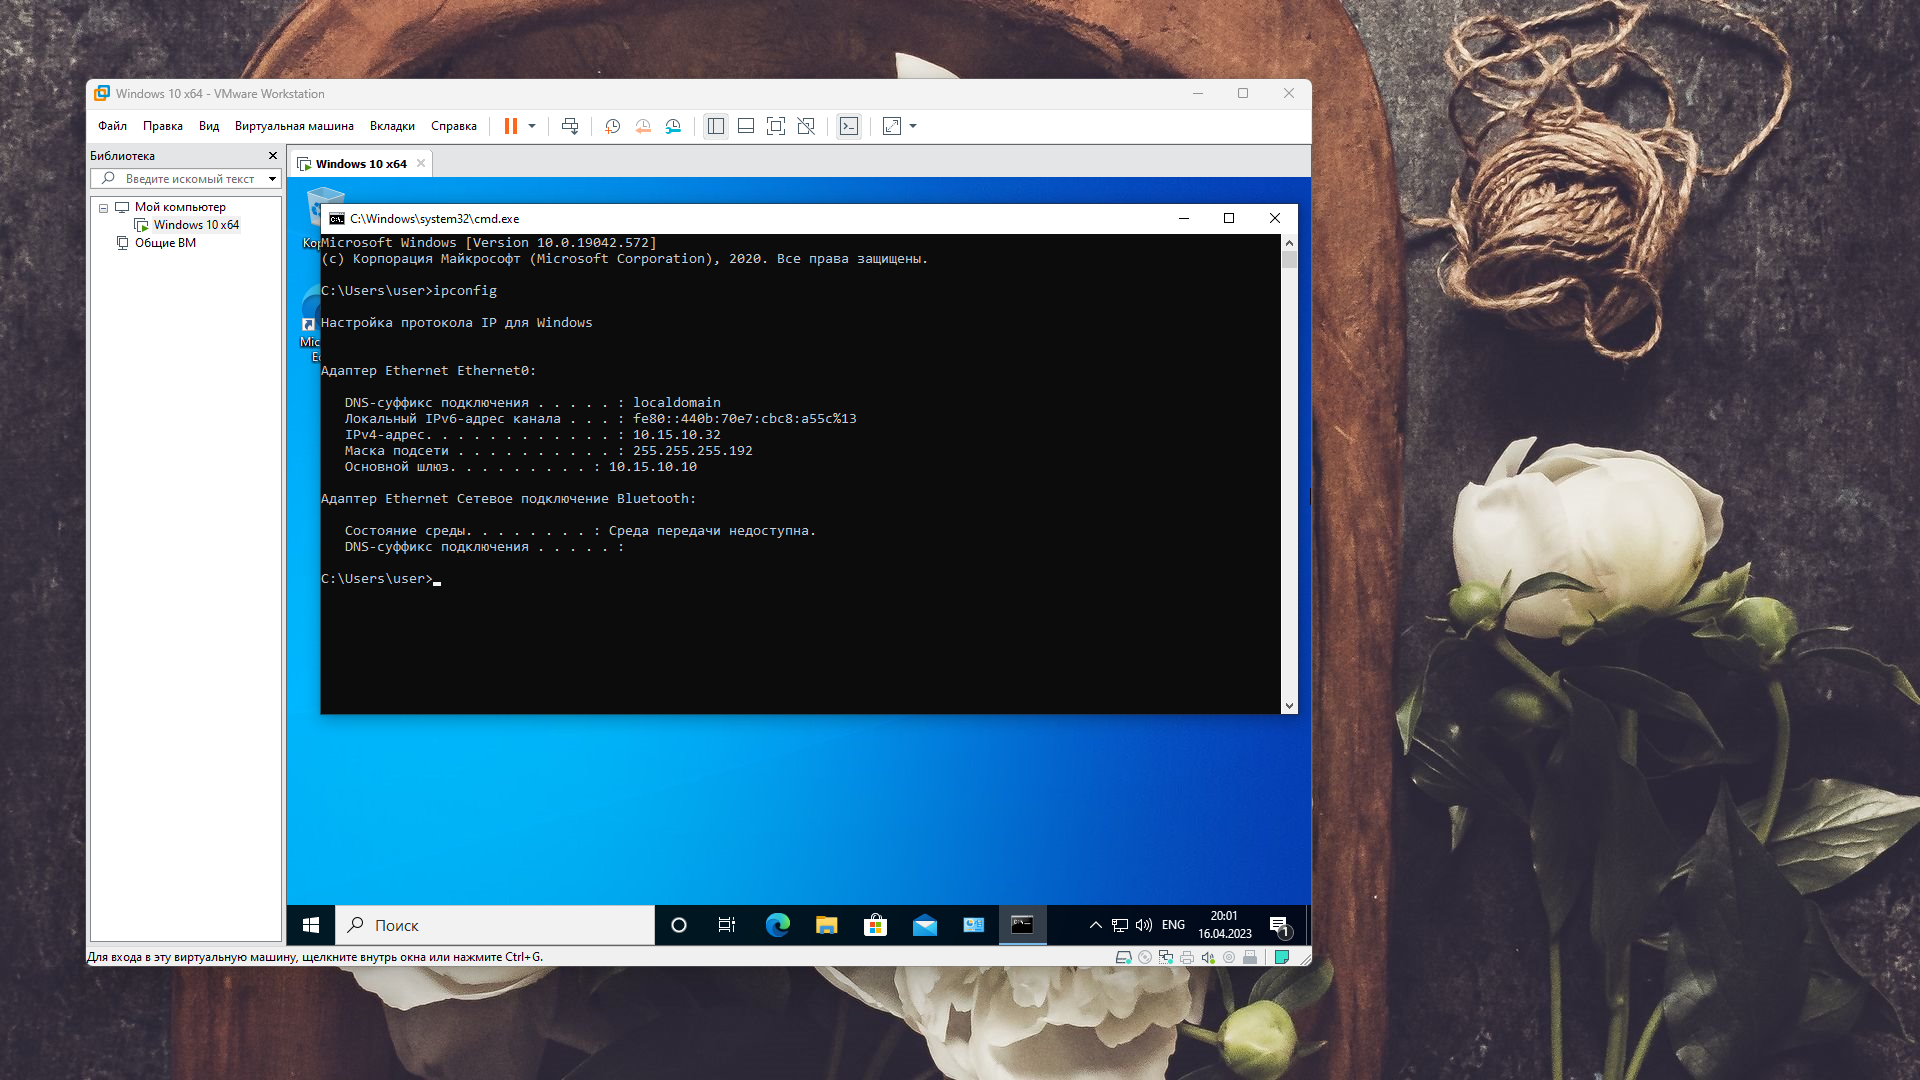
\includegraphics[width=0.85\textwidth]{06_00 (15)}
    \label{img:15}
    \caption{Узнаем текущие параметры сетевых интерфейсов при помощи команды \textit{ipconfig}}
  \end{figure}
  
  Видно, что встроенный в \textit{VMWare} \textit{DHCP} сервер отработал и выдал 
  текущей машине \textit{IPv4} адрес 10.15.10.32, а также правильно указал маску подсети
  и адрес шлюза - как и было указано ранее.

  Теперь нужно проверить, что виртуальная машина имеет доступ в сеть, для этого отправим
  пакеты на удаленный сервер, расположенный по адресу 8.8.8.8 при помощи утилиты \textit{ping}:
  
  Также можно удостовериться, что корректно отрабатывают \textit{DNS} пробы, и отправить
  пакеты по доменному имени, например на \href{ya.ru}{ya.ru}:

  \begin{figure}[H]
    \centering
    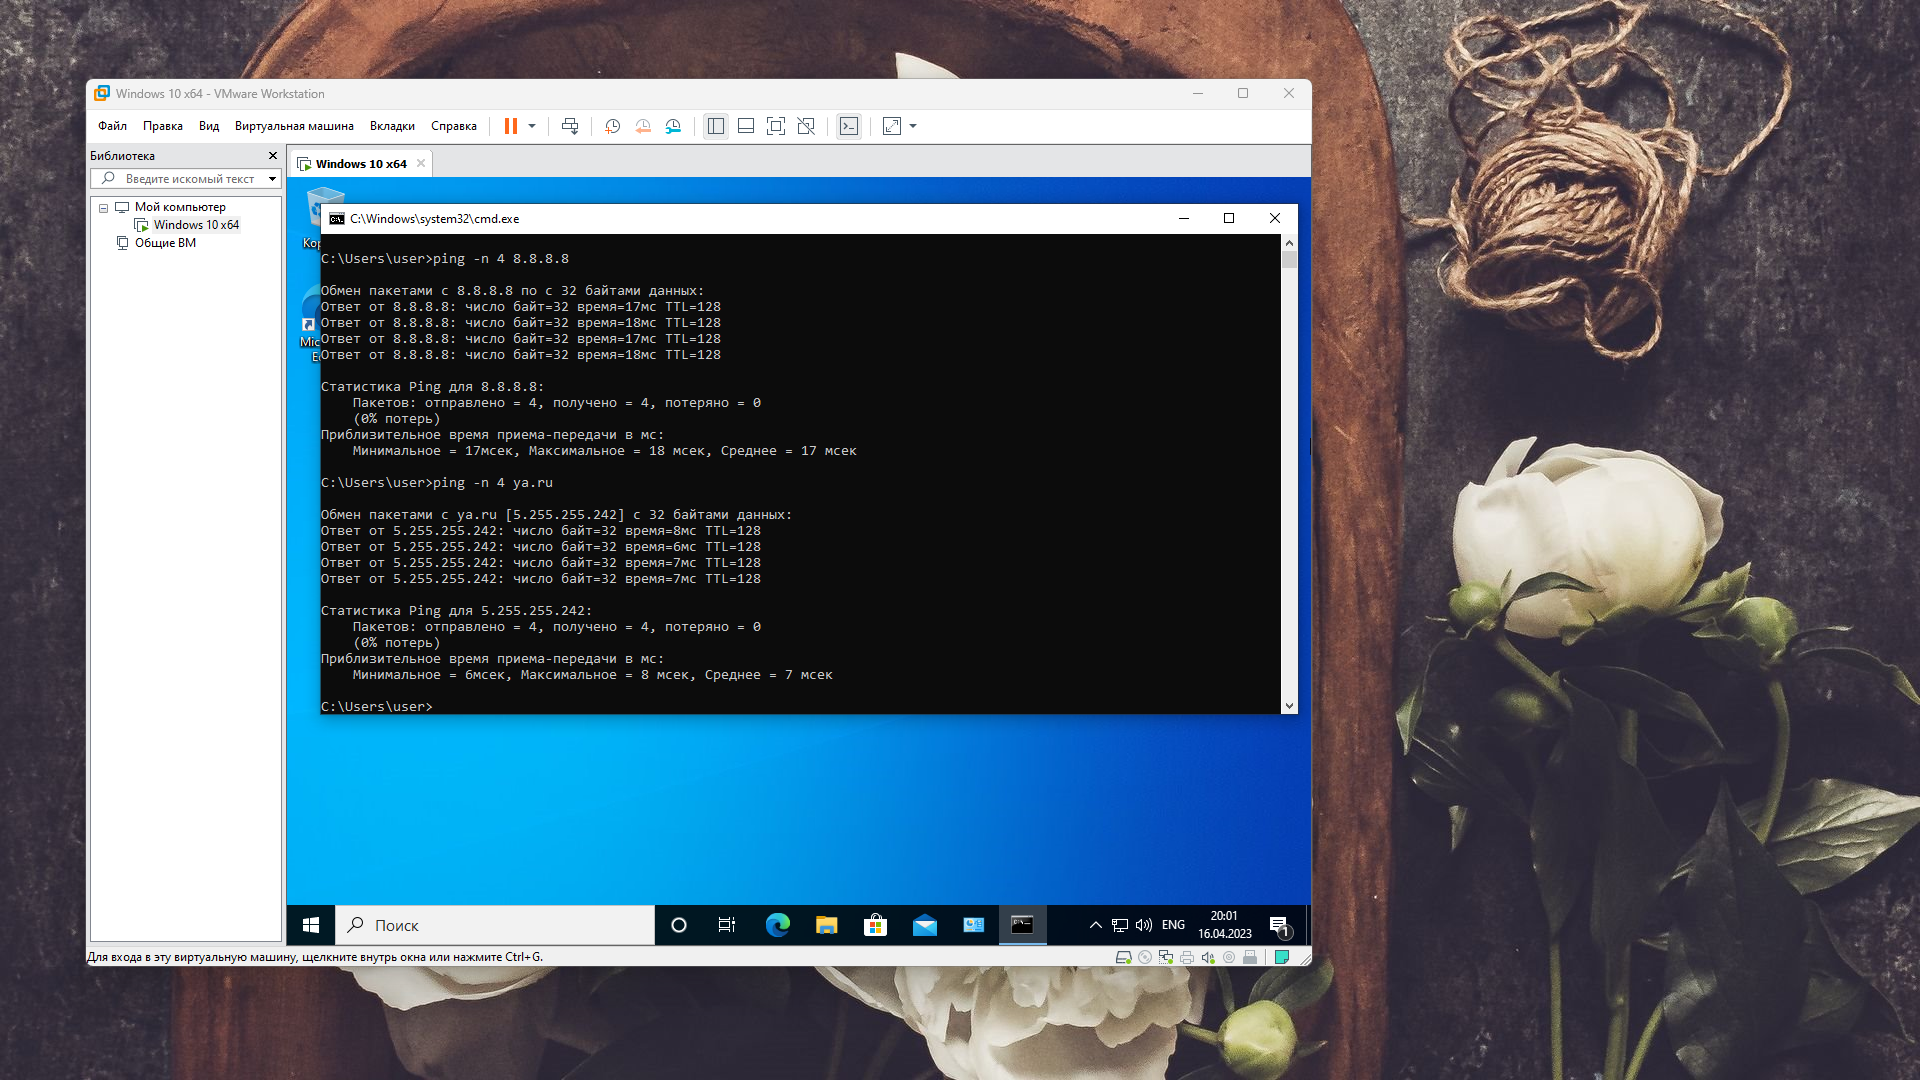
\includegraphics[width=0.85\textwidth]{06_00 (16)}
    \label{img:16}
    \caption{ping google dns и ya.ru}
  \end{figure}
  
  \subsubsection{Настройка статической адресации}
  
  Для начала необходимо отредактировать \textit{NAT} сеть - отключить \textit{DHCP} сервер,
  чтобы машины не могли самостоятельно получить \textit{IP} адрес. Для этого снова
  зайдем в настройки сетей:

  \begin{figure}[H]
    \centering
    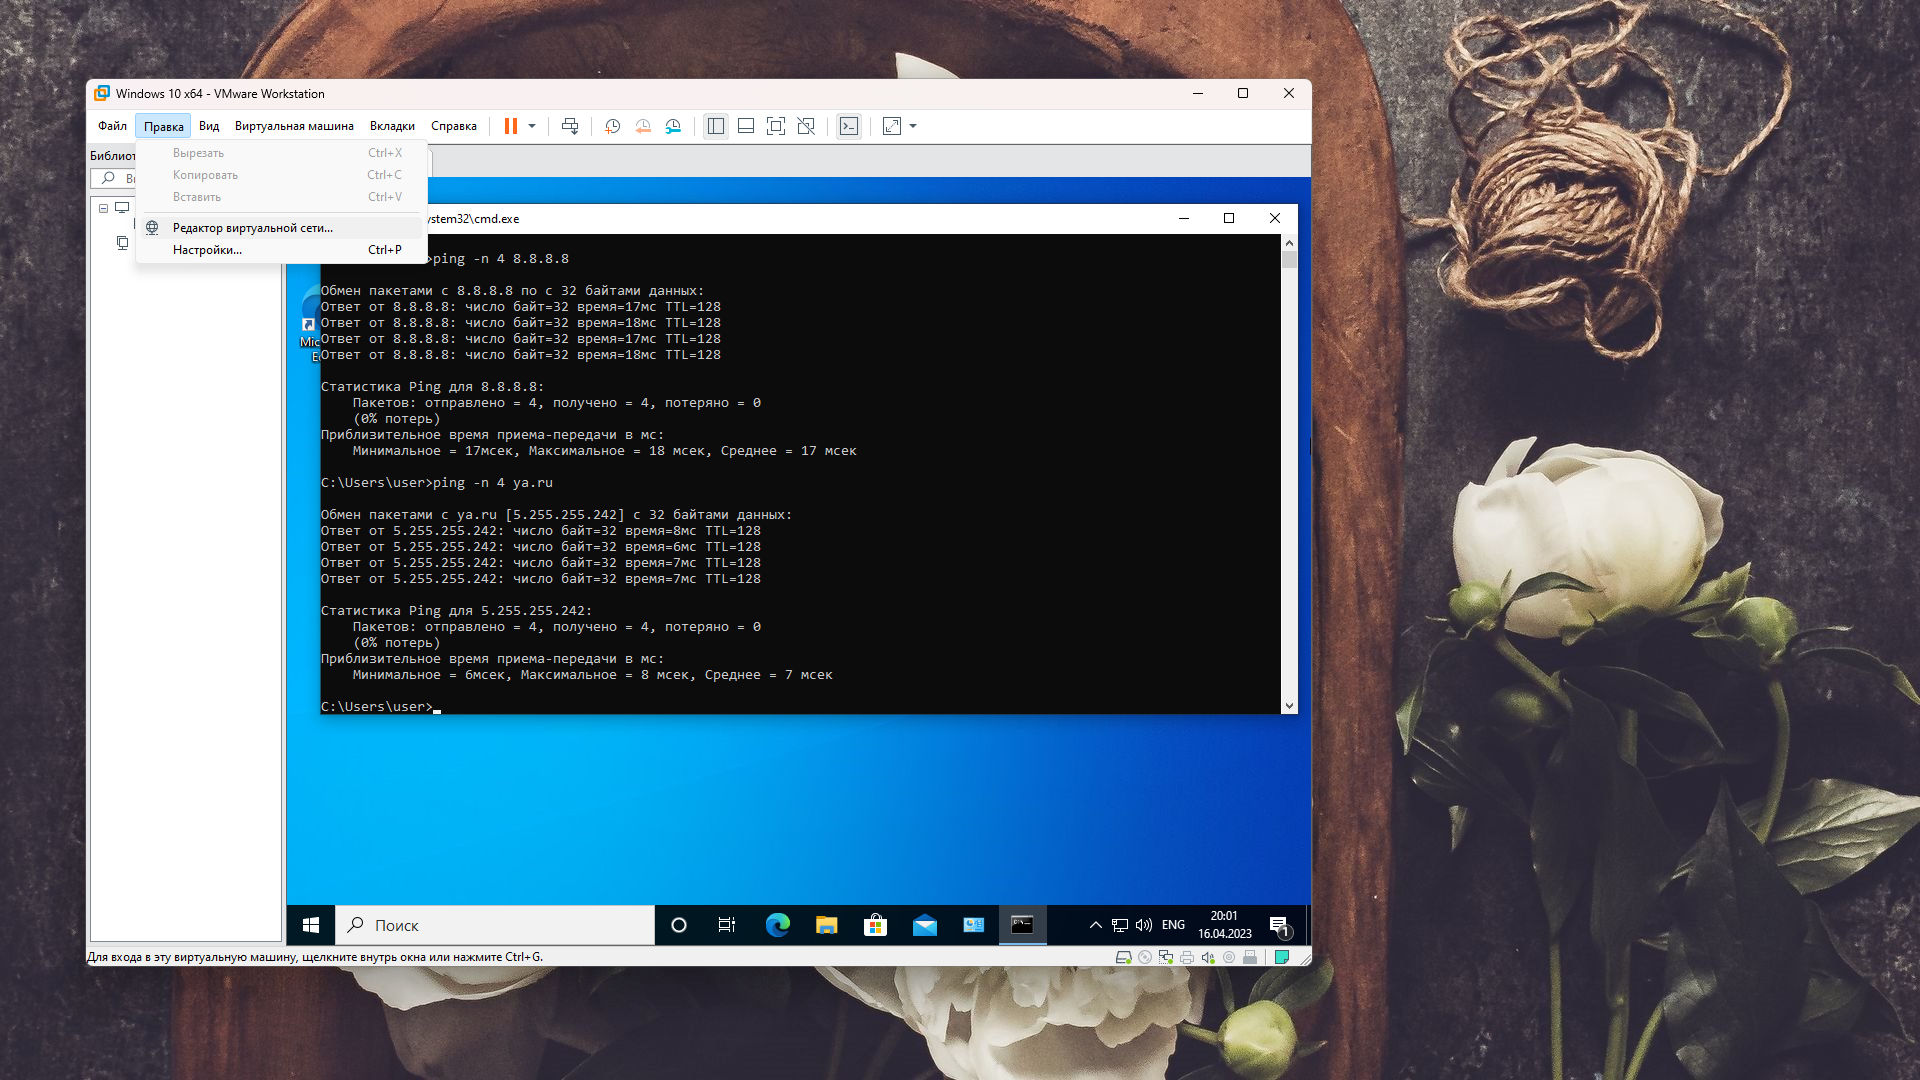
\includegraphics[width=0.85\textwidth]{06_00 (17)}
    \label{img:17}
    \caption{Открываем редактор виртульной сети}
  \end{figure}

  \begin{figure}[H]
    \centering
    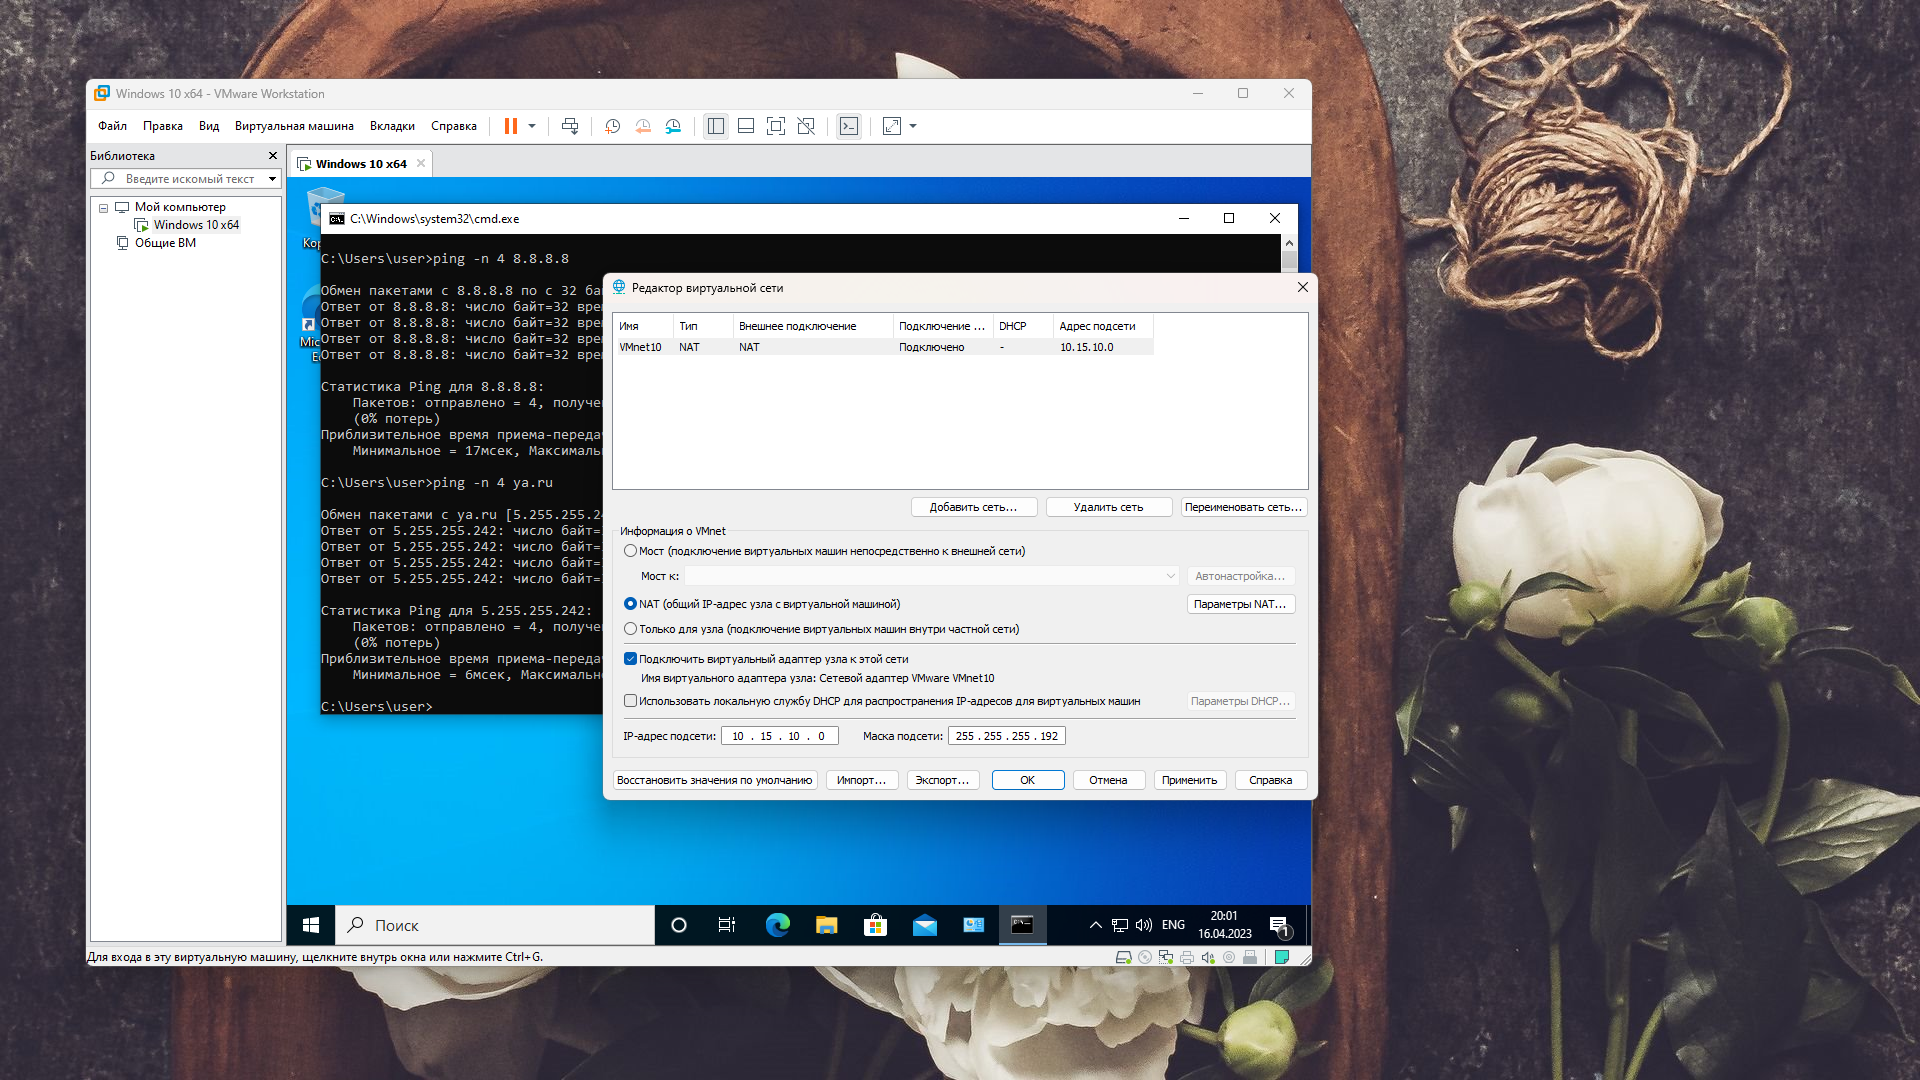
\includegraphics[width=0.85\textwidth]{06_00 (18)}
    \label{img:18}
    \caption{Отключаем \textit{DHCP} сервер}
  \end{figure}
  
  Далее необходимо вручную задать \textit{IP} адрес на виртуальной машине:

  \begin{figure}[H]
    \centering
    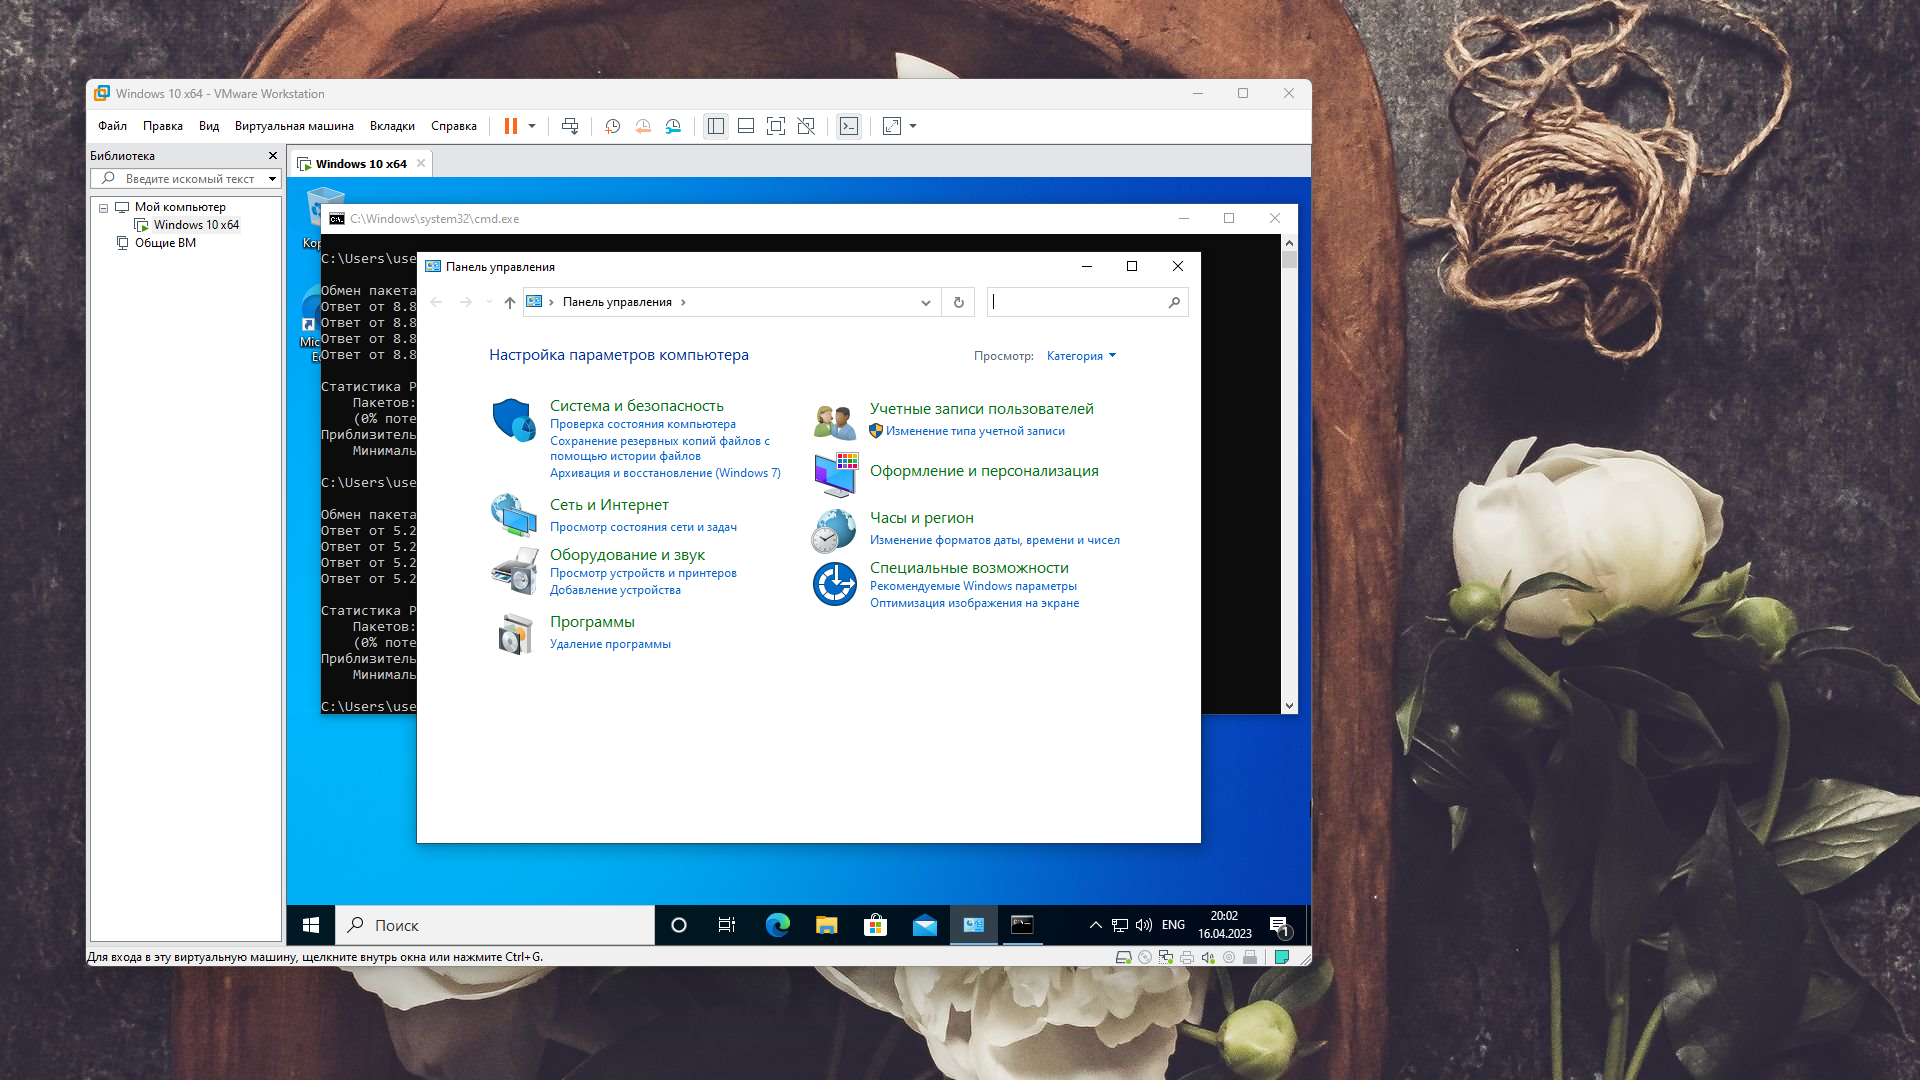
\includegraphics[width=0.85\textwidth]{06_00 (19)}
    \label{img:19}
    \caption{Открываем Панель задач}
  \end{figure}
  
  \begin{figure}[H]
    \centering
    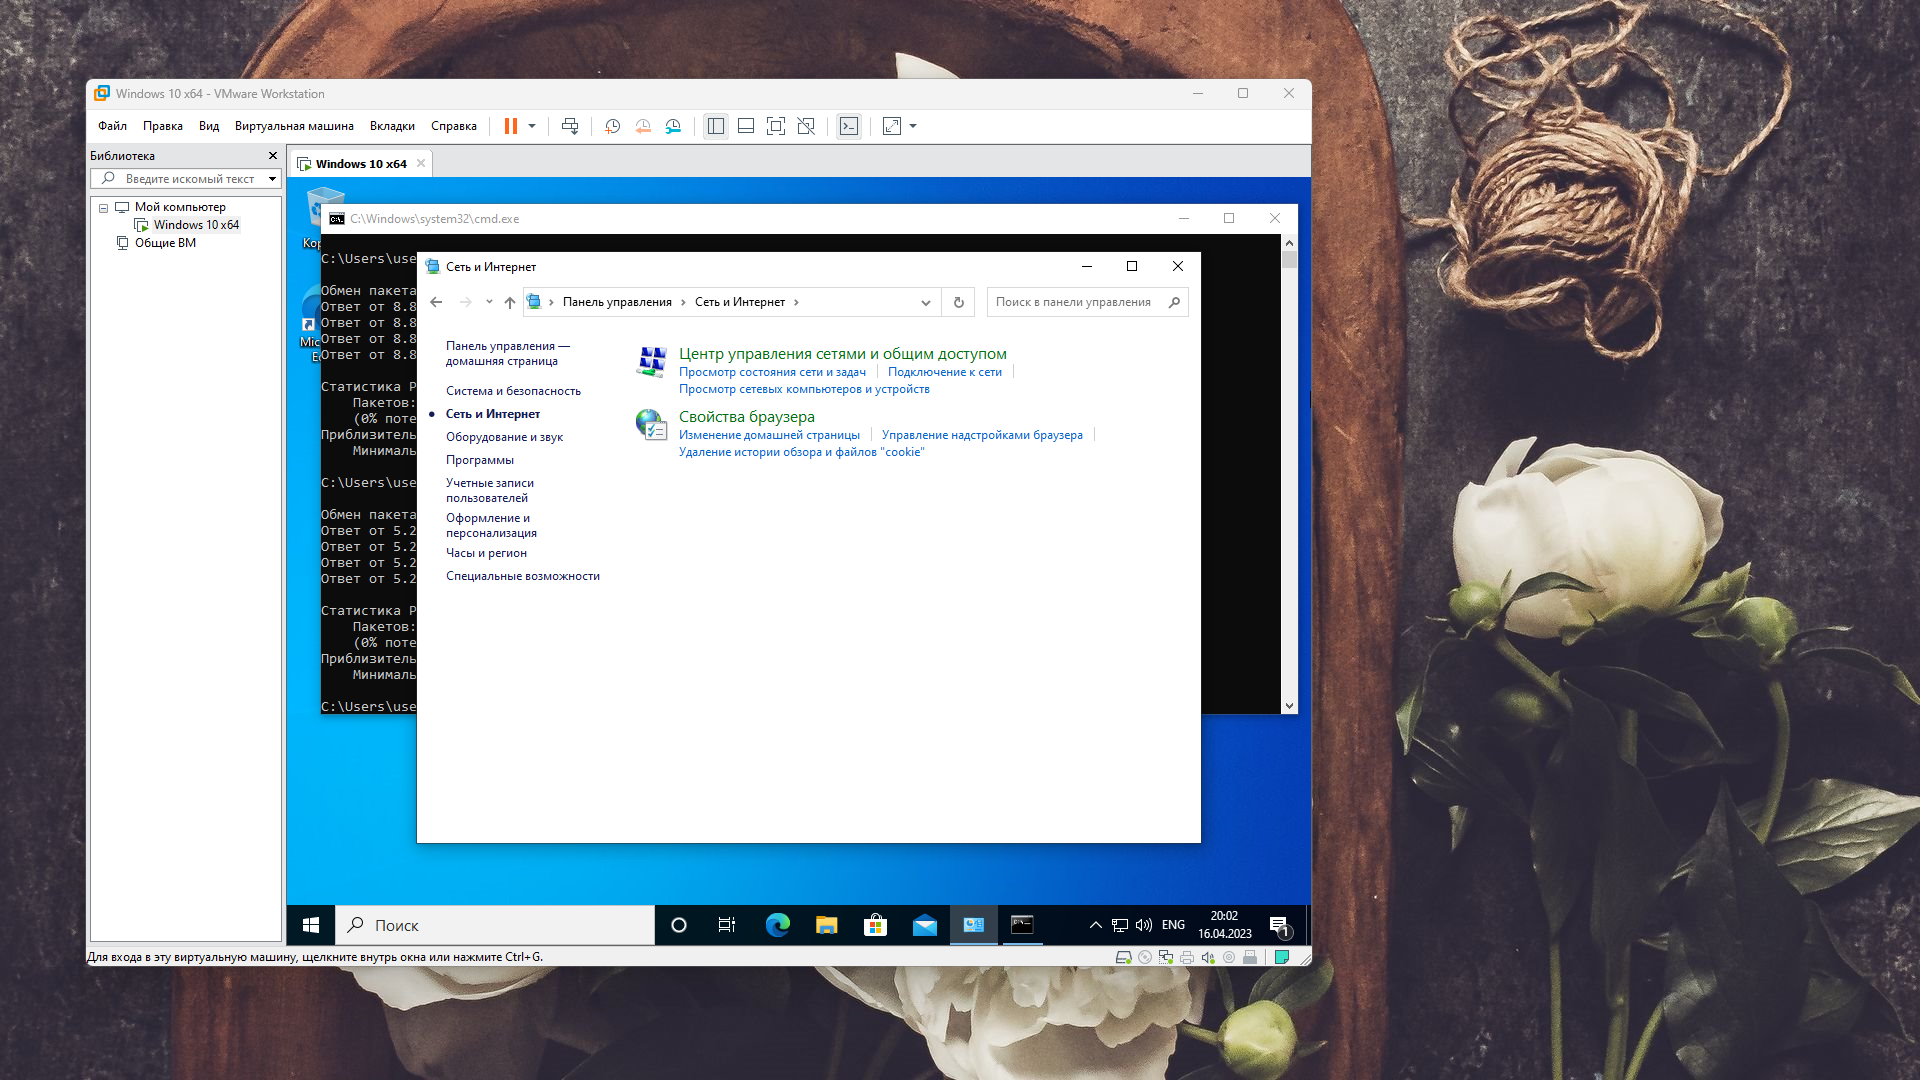
\includegraphics[width=0.85\textwidth]{06_00 (20)}
    \label{img:20}
    \caption{Пункт "Сеть и Интернет"}
  \end{figure}
  
  \begin{figure}[H]
    \centering
    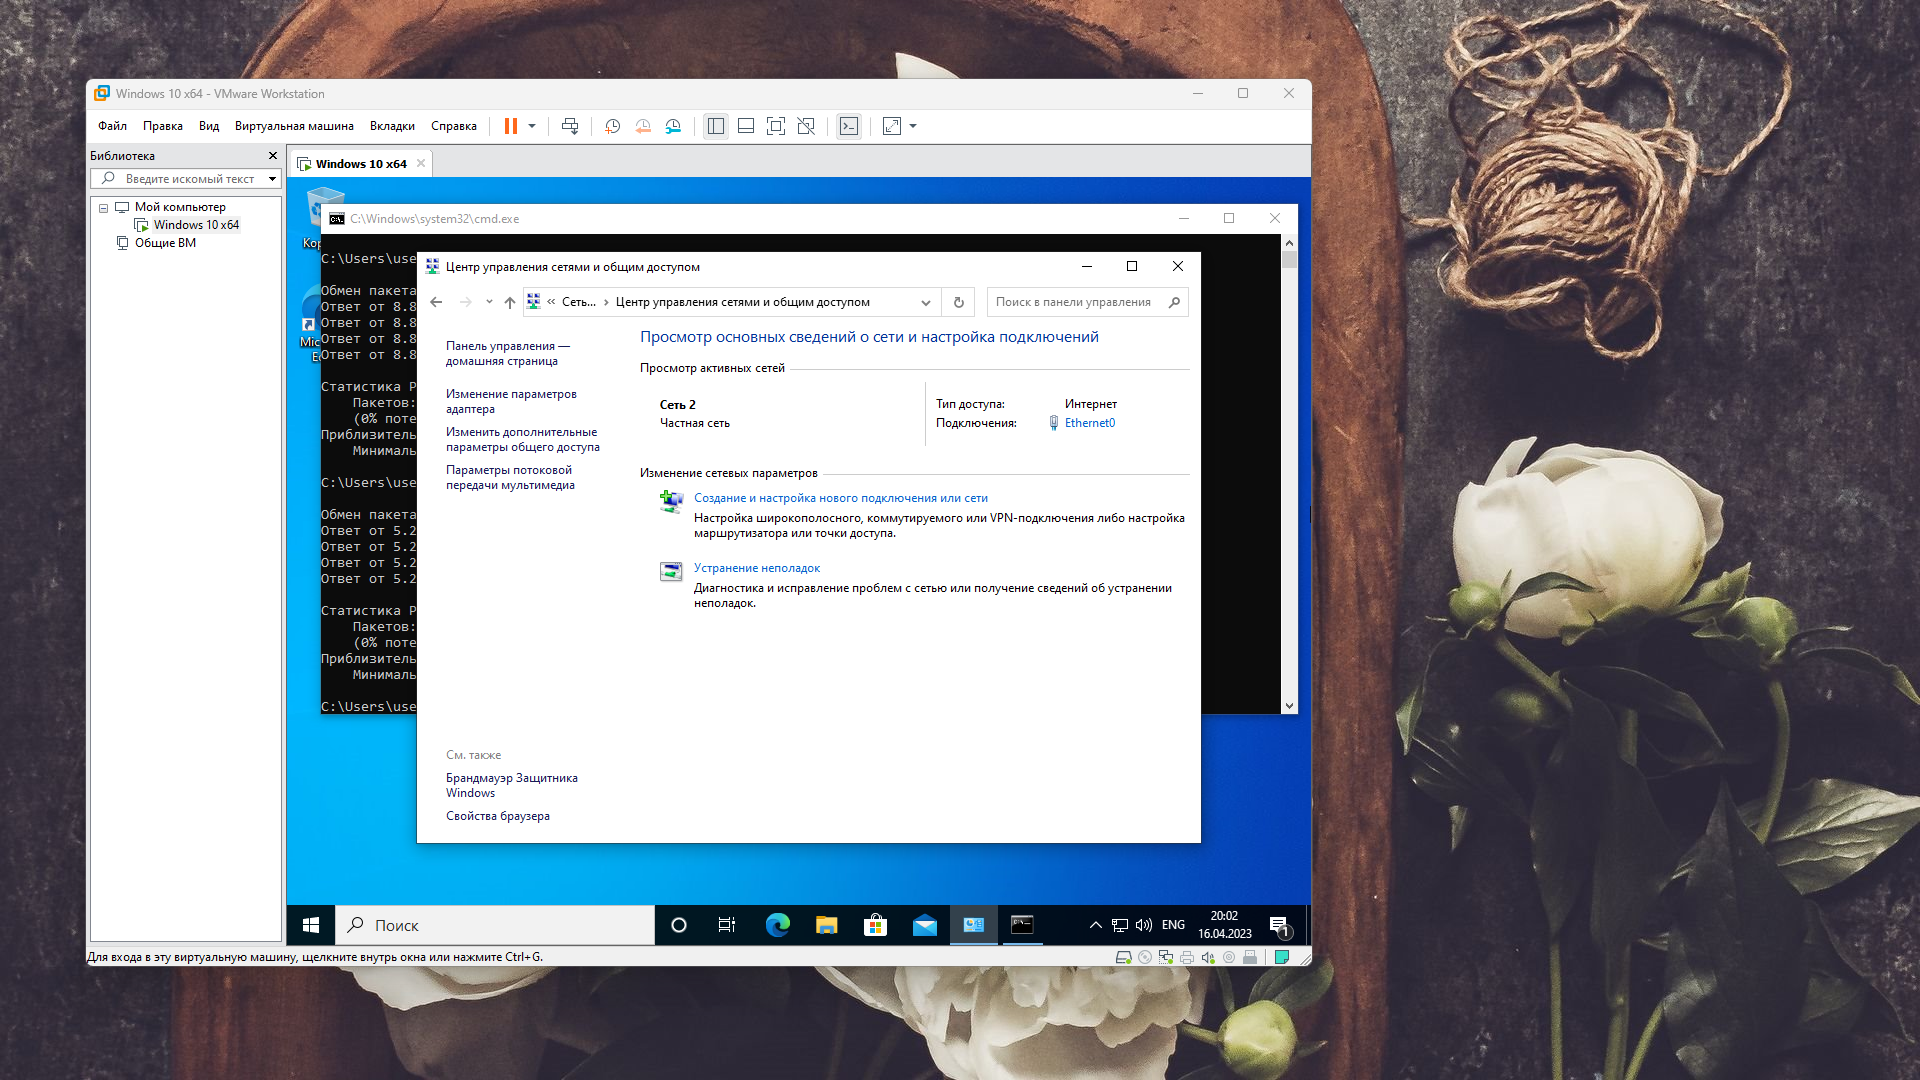
\includegraphics[width=0.85\textwidth]{06_00 (21)}
    \label{img:21}
    \caption{Пункт "Центр управления сетями и общим доступом"}
  \end{figure}
  
  \begin{figure}[H]
    \centering
    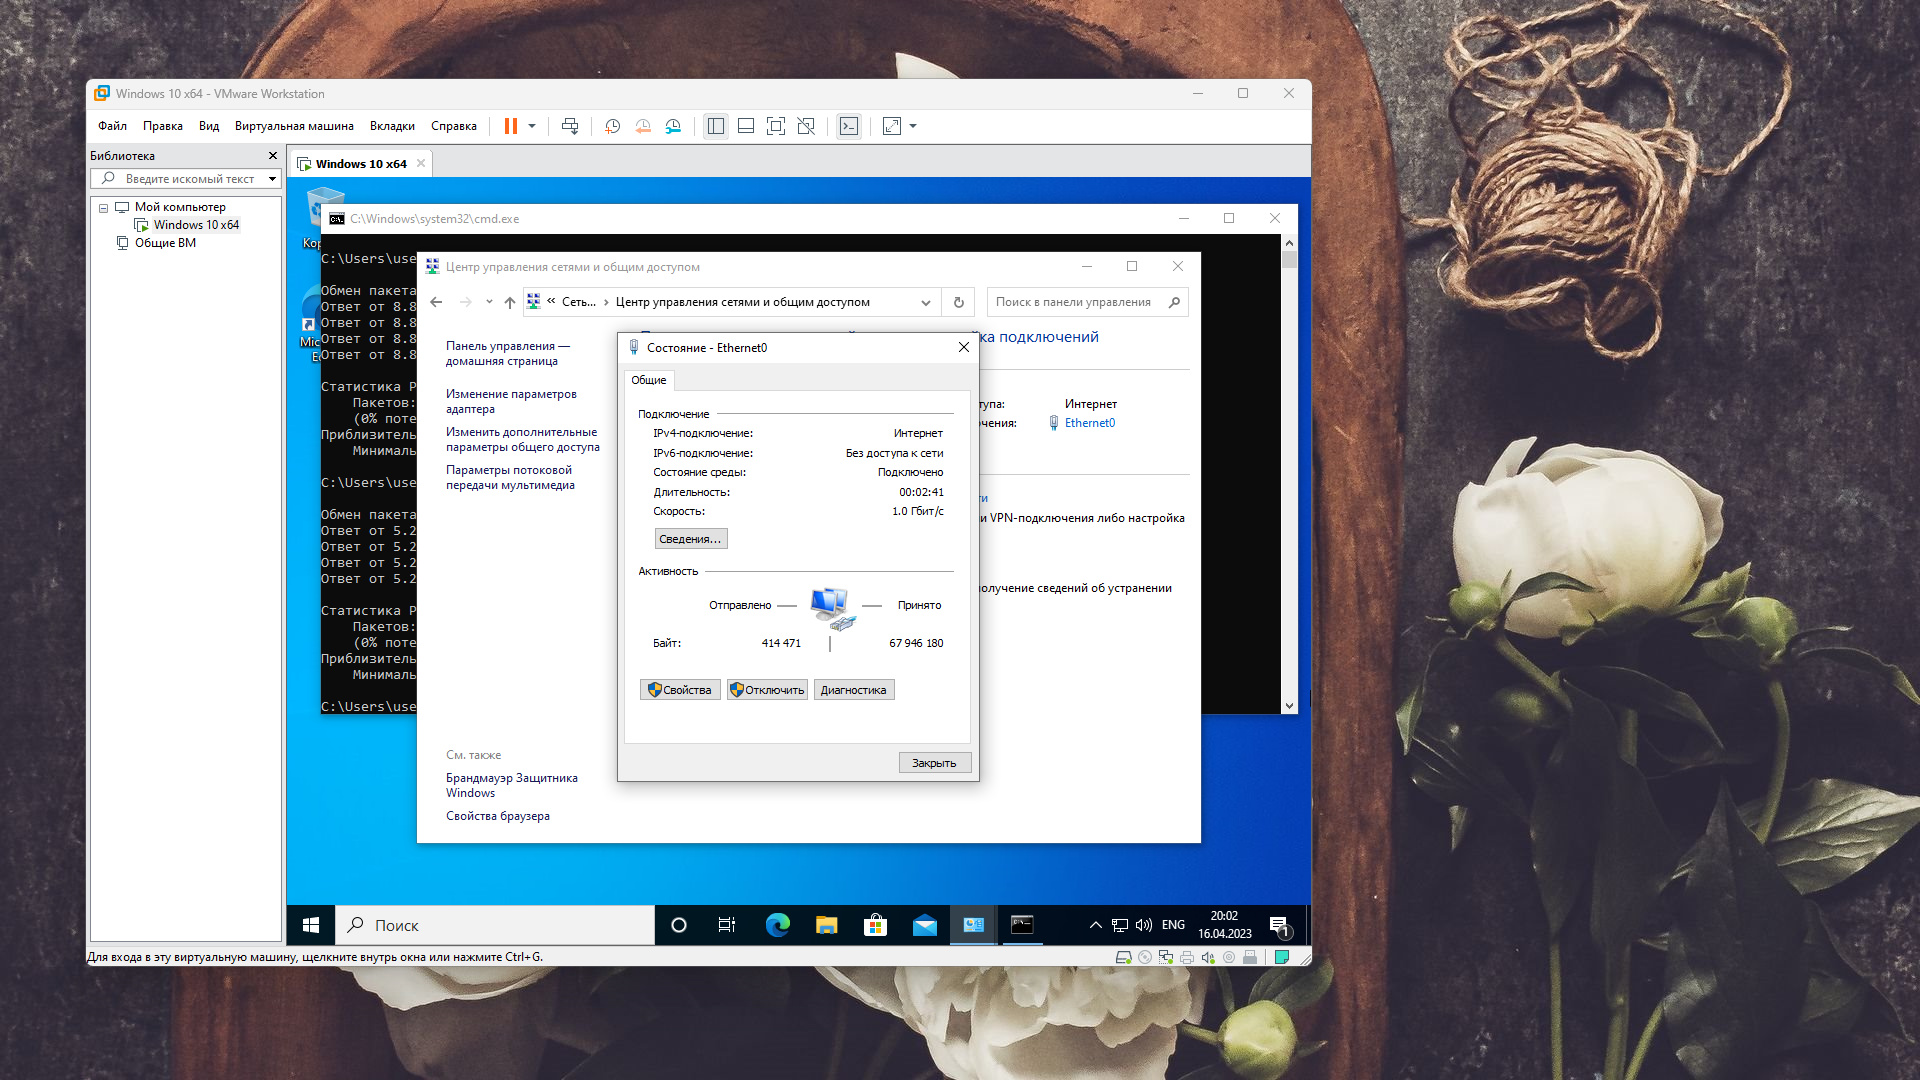
\includegraphics[width=0.85\textwidth]{06_00 (22)}
    \label{img:22}
    \caption{Выбираем единственный доступный сетевой адаптер - Ethernet0}
  \end{figure}
  
  \begin{figure}[H]
    \centering
    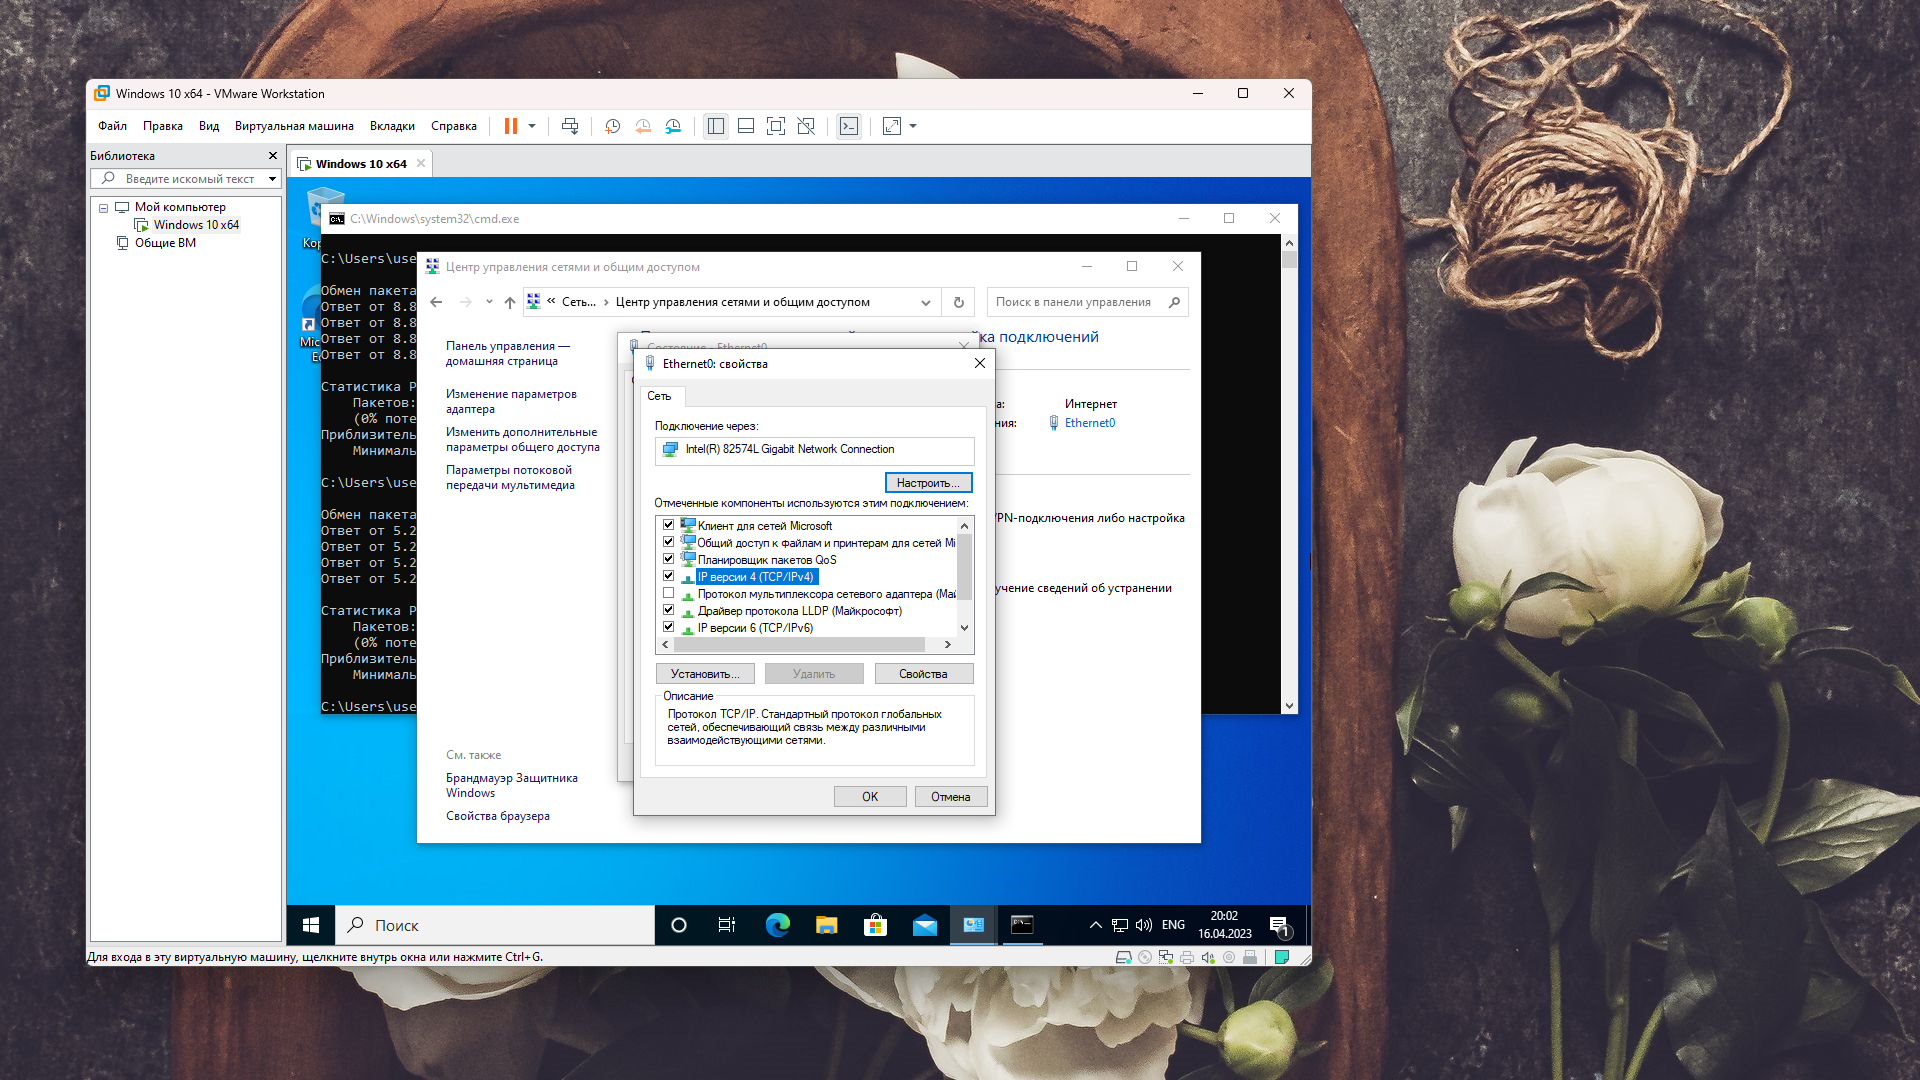
\includegraphics[width=0.85\textwidth]{06_00 (23)}
    \label{img:23}
    \caption{В его свойствах ищем пункт \textit{IPv4} и открываем его}
  \end{figure}
  
  \begin{figure}[H]
    \centering
    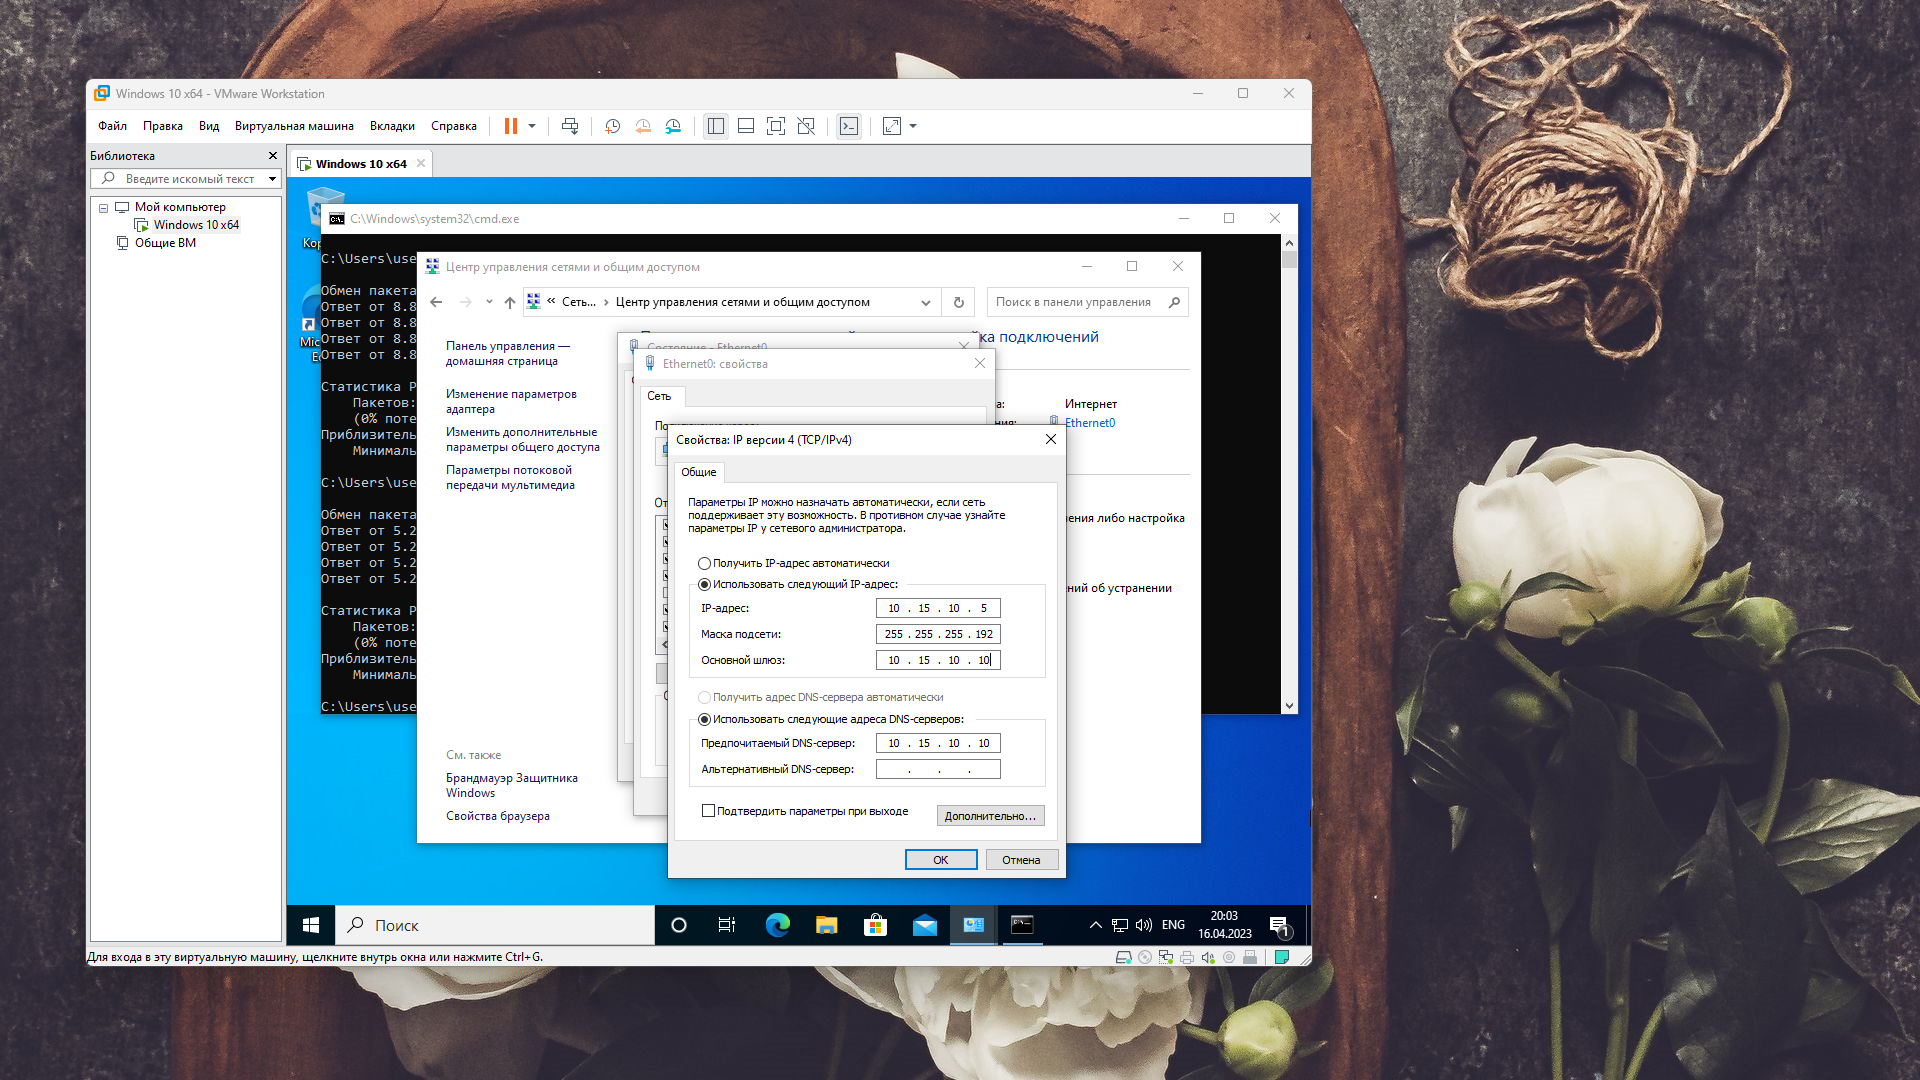
\includegraphics[width=0.85\textwidth]{06_00 (24)}
    \label{img:24}
    \caption{Вручную задаем необходимые параметры}
  \end{figure}

  Для данной виртуальной машины я выбрал адрес 10.15.10.5:
  
  \begin{figure}[H]
    \centering
    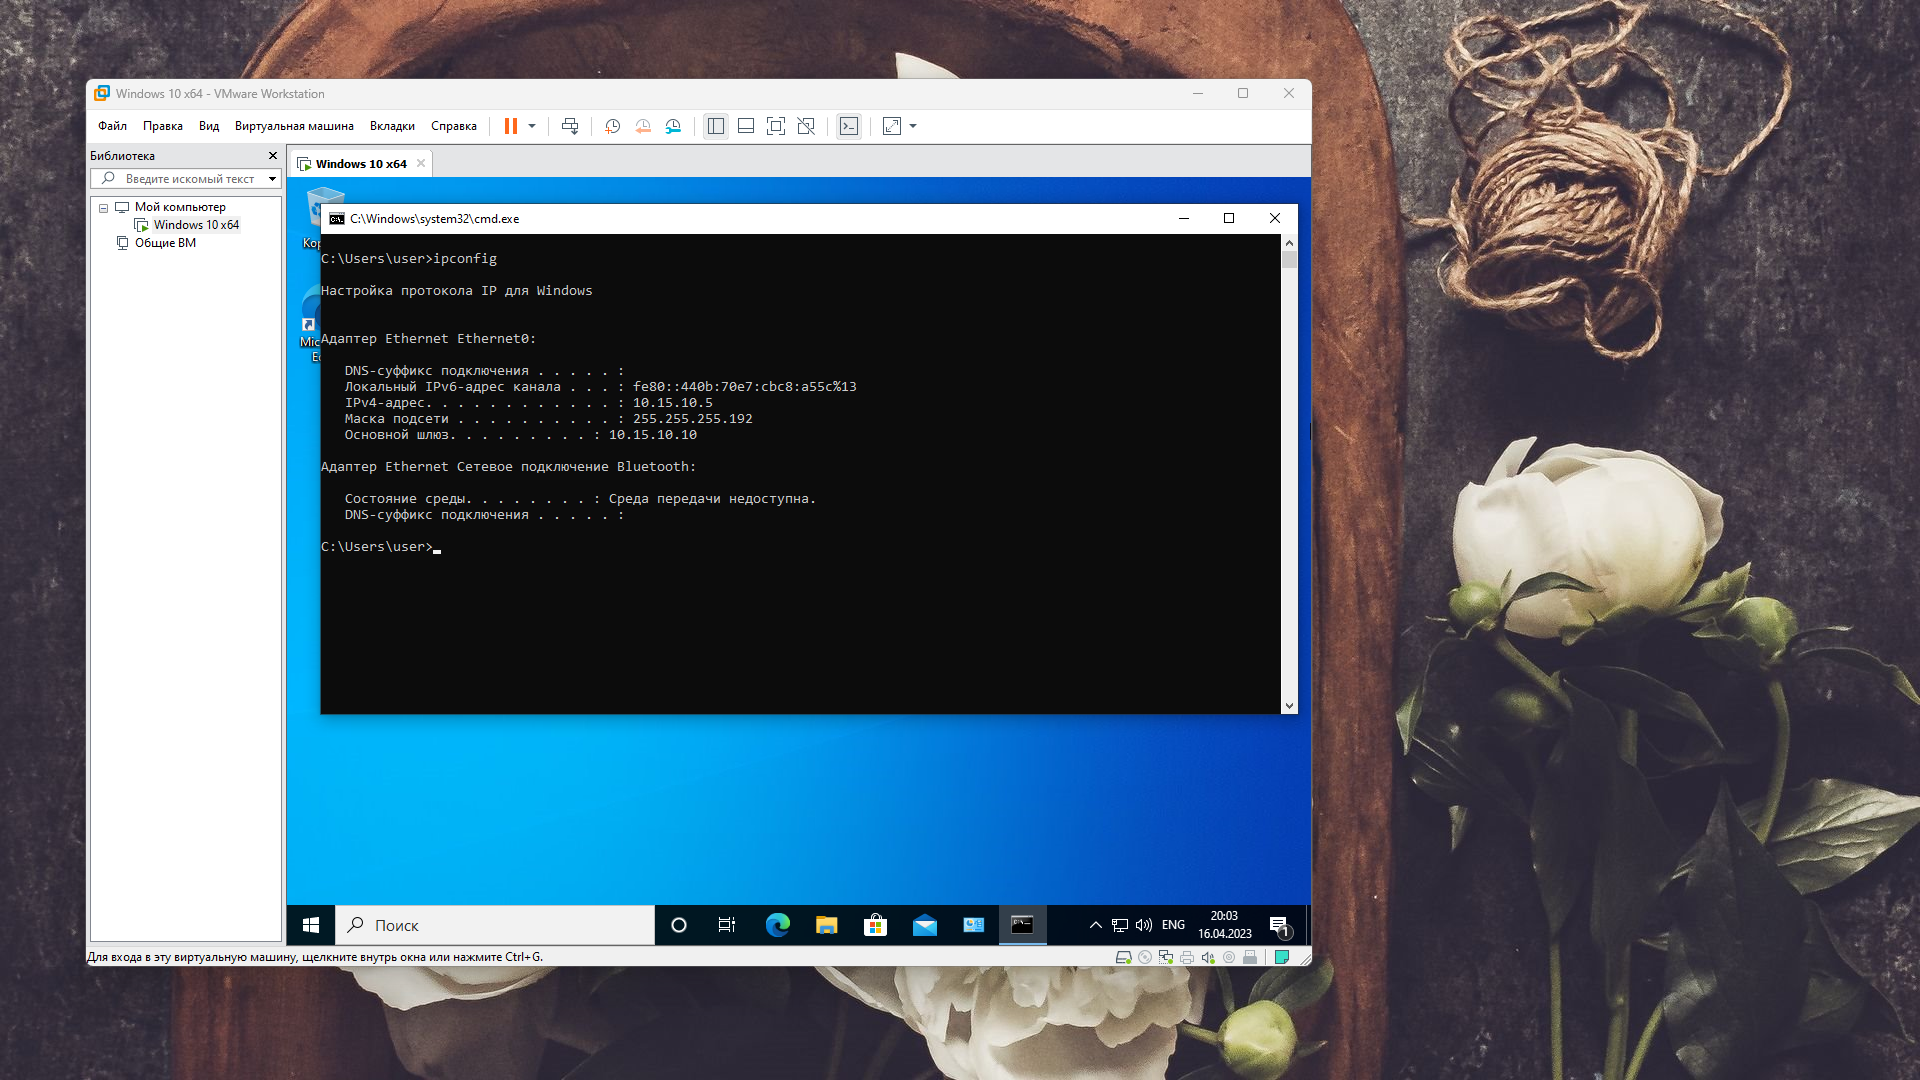
\includegraphics[width=0.85\textwidth]{06_00 (25)}
    \label{img:25}
    \caption{Выполняем проверку при помощи \textit{ipconfig}}
  \end{figure}
  
  Теперь необходимо удостовериться, что у машины есть возможность подключиться
  к шлюзу по умолчанию (10.15.10.10):

  \begin{figure}[H]
    \centering
    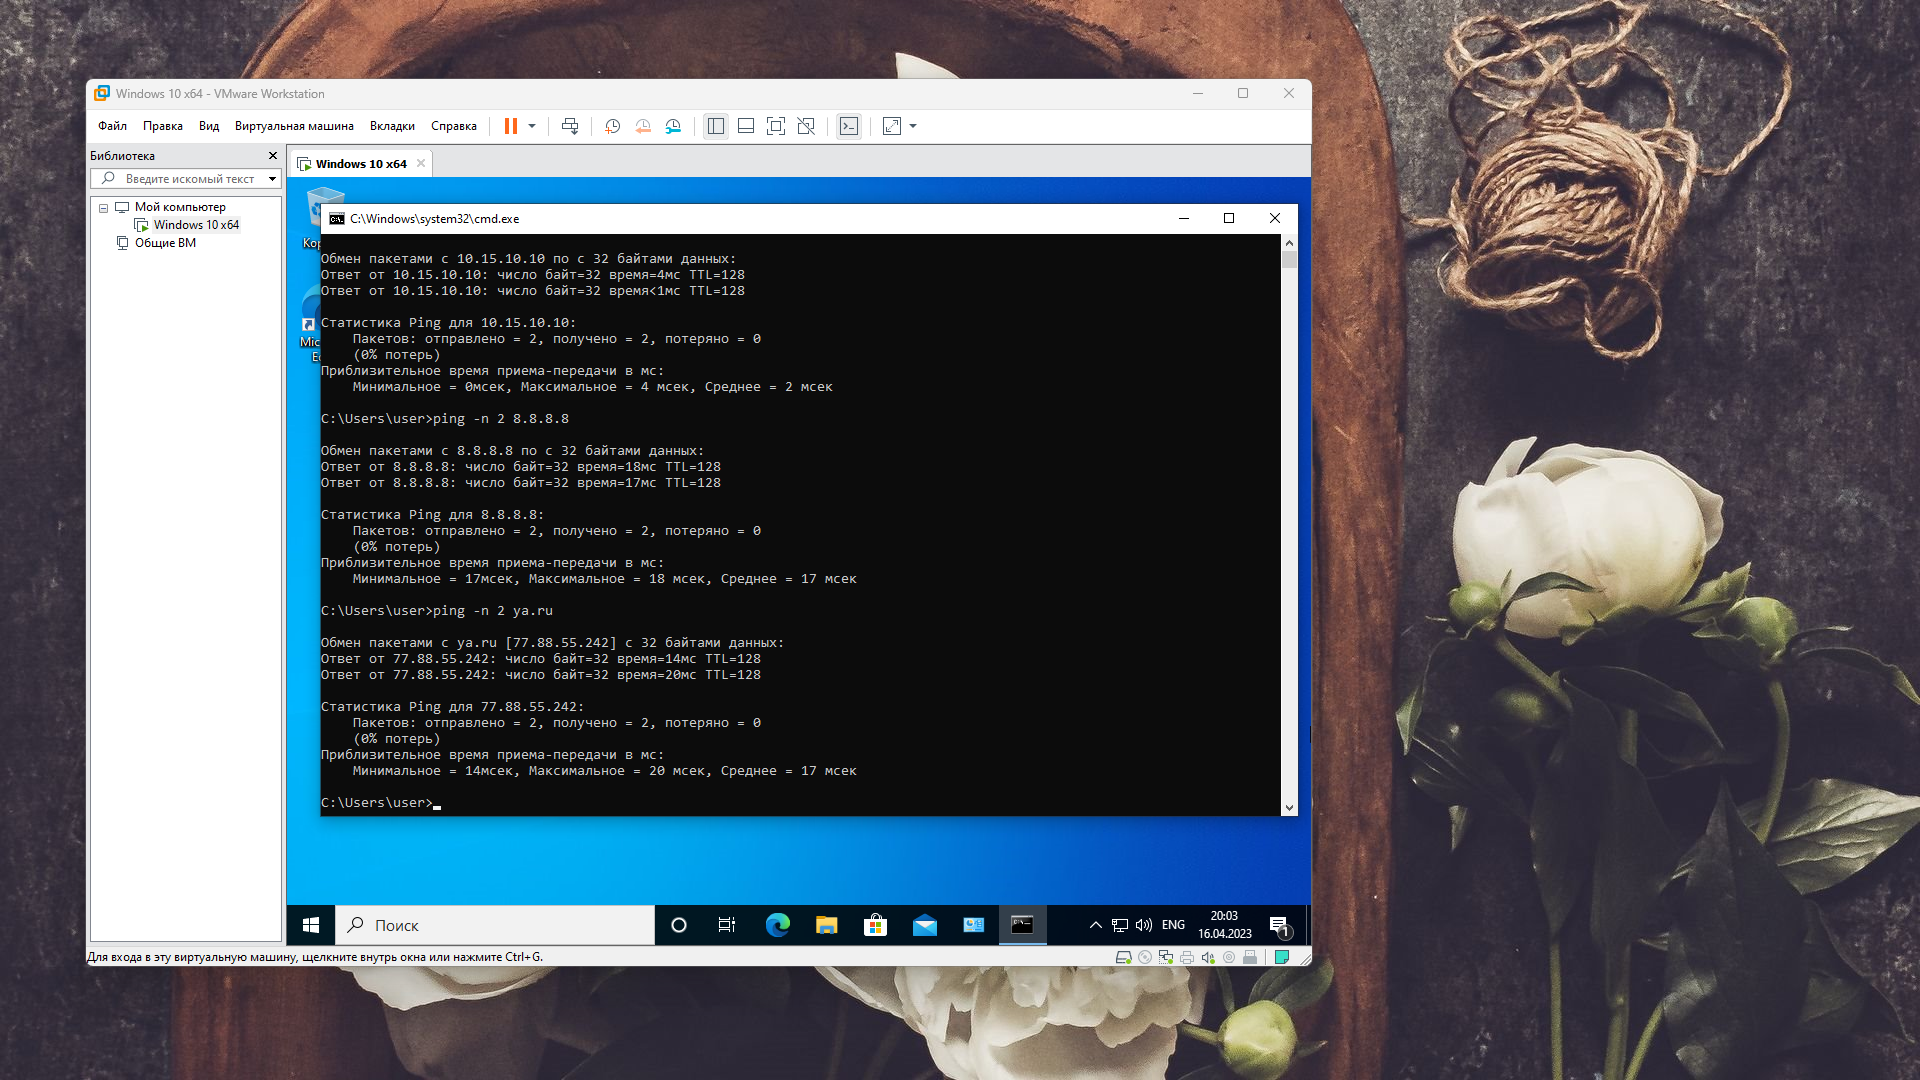
\includegraphics[width=0.85\textwidth]{06_00 (26)}
    \label{img:26}
    \caption{Проверка доступности при помощи \textit{ping}}
  \end{figure}

  Все пакеты отправлены и получены, следовательно настройка сети выполнена правильно.

  \subsubsection{Создание ВМ с Linux}

  Снова воспользуемся готовым образом:
  
  \begin{figure}[H]
    \centering
    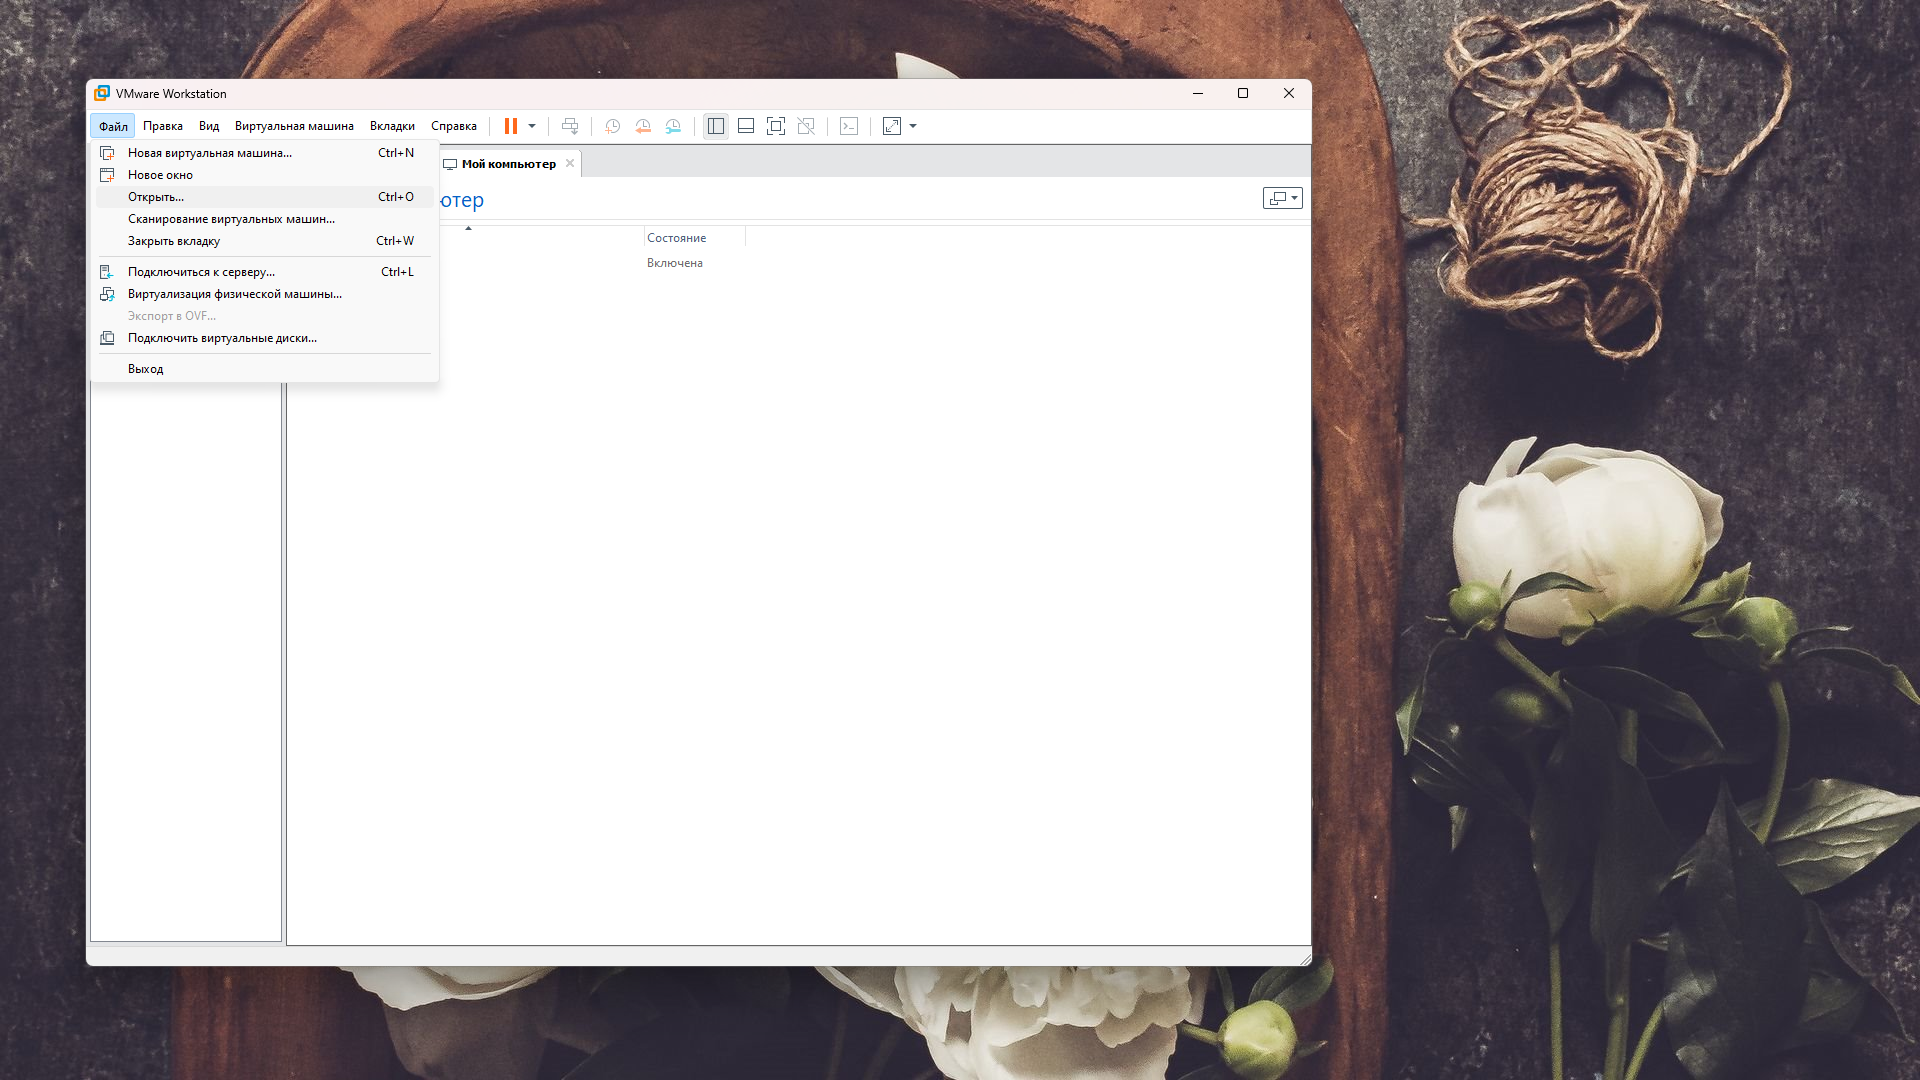
\includegraphics[width=0.85\textwidth]{06_00 (27)}
    \label{img:27}
    \caption{Выбираем пункт "Открыть"}
  \end{figure}
  
  \begin{figure}[H]
    \centering
    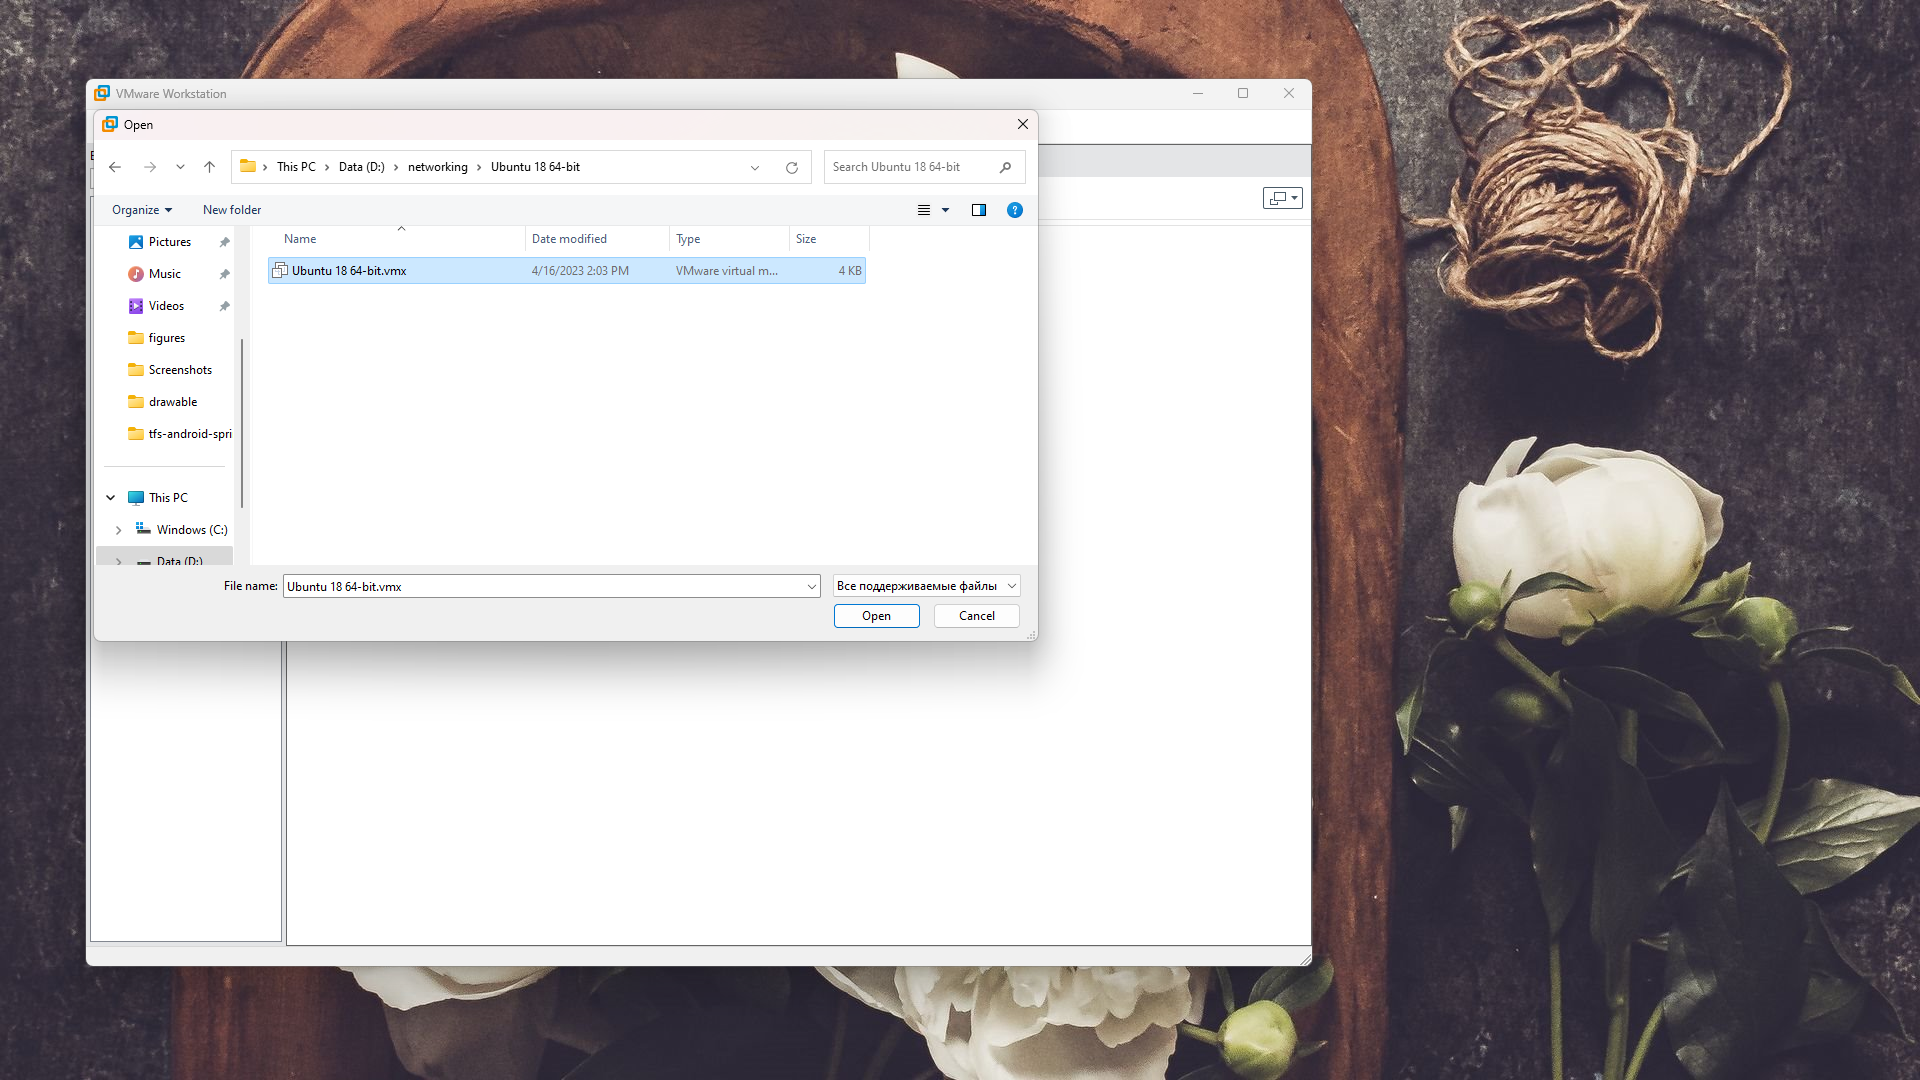
\includegraphics[width=0.85\textwidth]{06_00 (28)}
    \label{img:28}
    \caption{Указываем необходимый образ}
  \end{figure}
  
  Виртуальная машина создана, теперь необходимо подключить ее к нужной сети,
  для этого открываем ее настройки и добавляем новый сетевой адаптер:

  \begin{figure}[H]
    \centering
    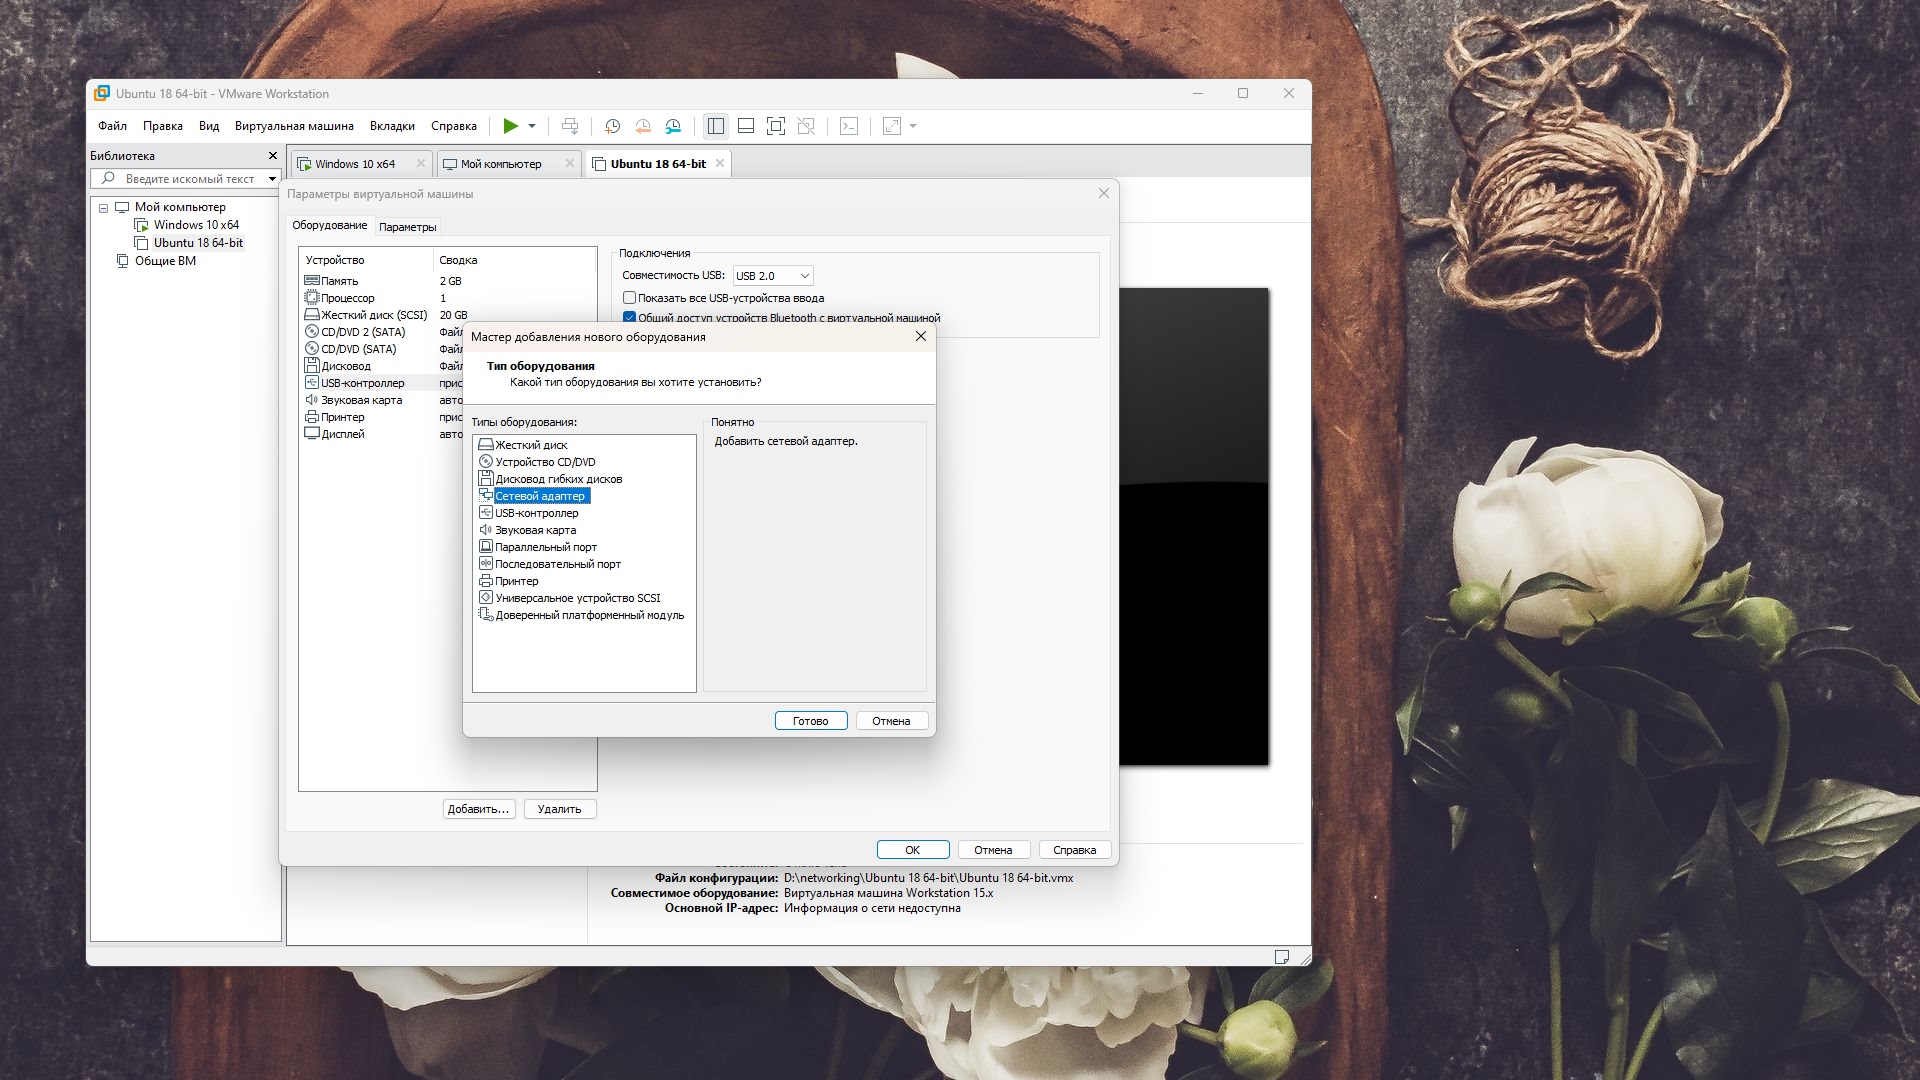
\includegraphics[width=0.85\textwidth]{06_00 (29)}
    \label{img:29}
    \caption{Создаем новый сетевой адаптер}
  \end{figure}
  
  \begin{figure}[H]
    \centering
    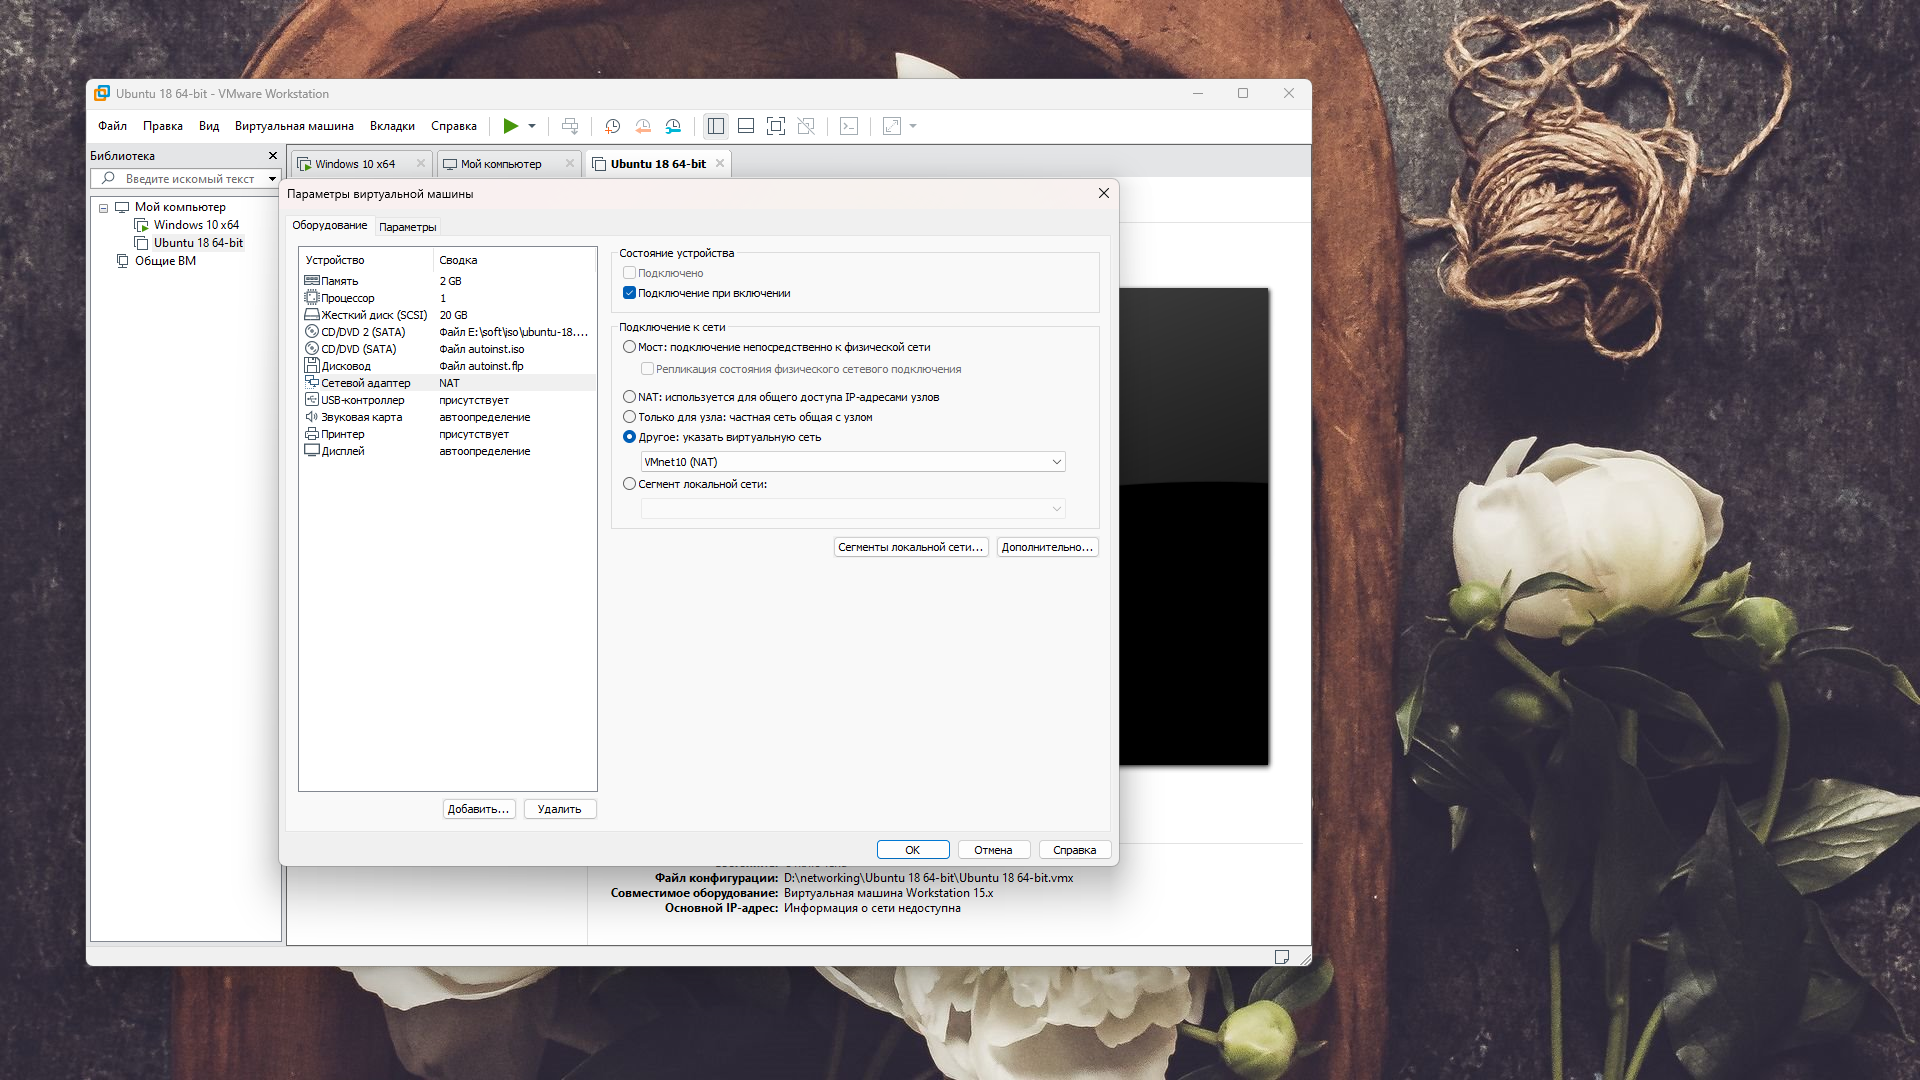
\includegraphics[width=0.85\textwidth]{06_00 (30)}
    \label{img:30}
    \caption{Подключаем его к нужной сети}
  \end{figure}

  Виртуальная машина создана и готова к работе.

  \subsubsection{Настройка статической адресации в Linux}
  
  \begin{figure}[H]
    \centering
    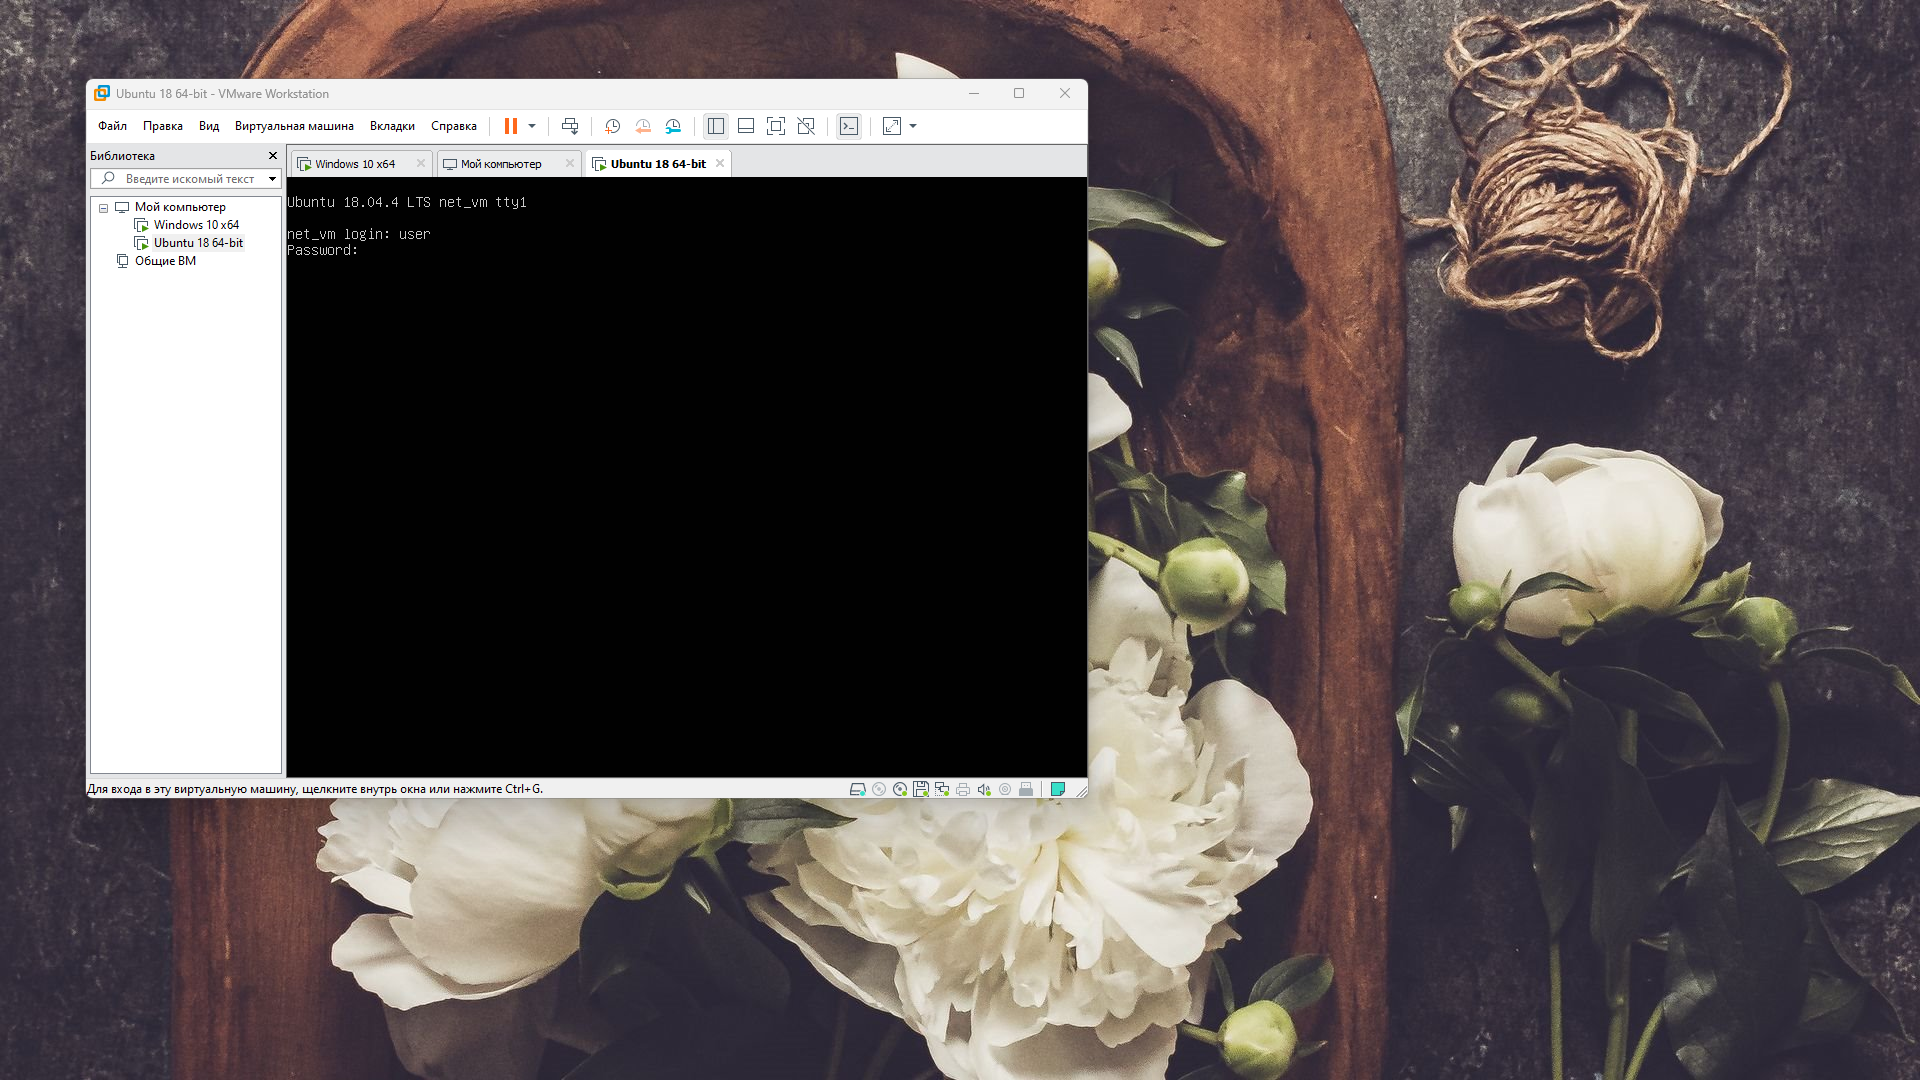
\includegraphics[width=0.85\textwidth]{06_00 (31)}
    \label{img:31}
    \caption{Входим в учетную запись пользователя}
  \end{figure}
  
  Для настройки необходима утилита \textit{netplan}, к счастью, она уже установлена
  и дополнительные действия не требуются, однако, если бы ее не было, то это можно 
  было бы исправить с помощью следующей команды:
  \mint{bash}|sudo apt install netplan|

  \begin{figure}[H]
    \centering
    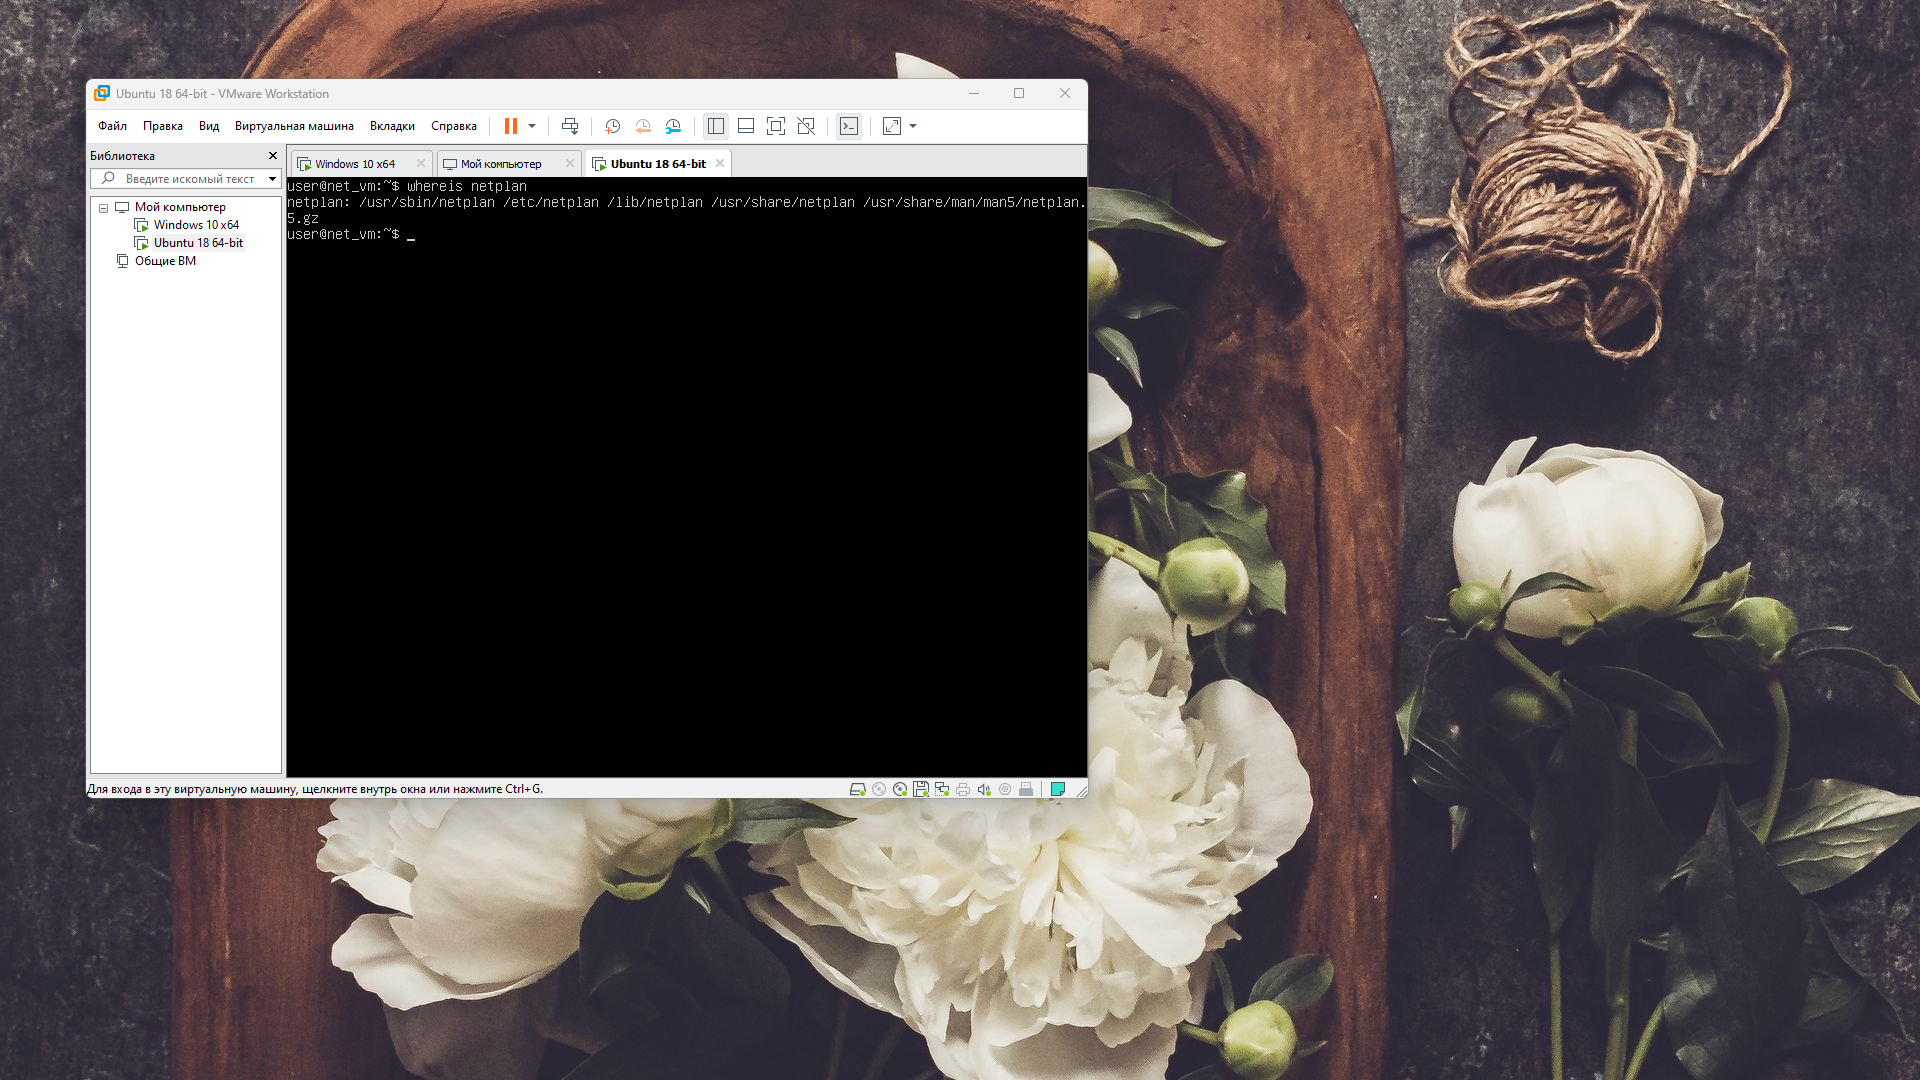
\includegraphics[width=0.85\textwidth]{06_00 (32)}
    \label{img:32}
    \caption{Проверка наличия \textit{netplan} в системе}
  \end{figure}
  
  Настройка выполняется при помощи специального конфигурационного файла, откроем его:

  \begin{figure}[H]
    \centering
    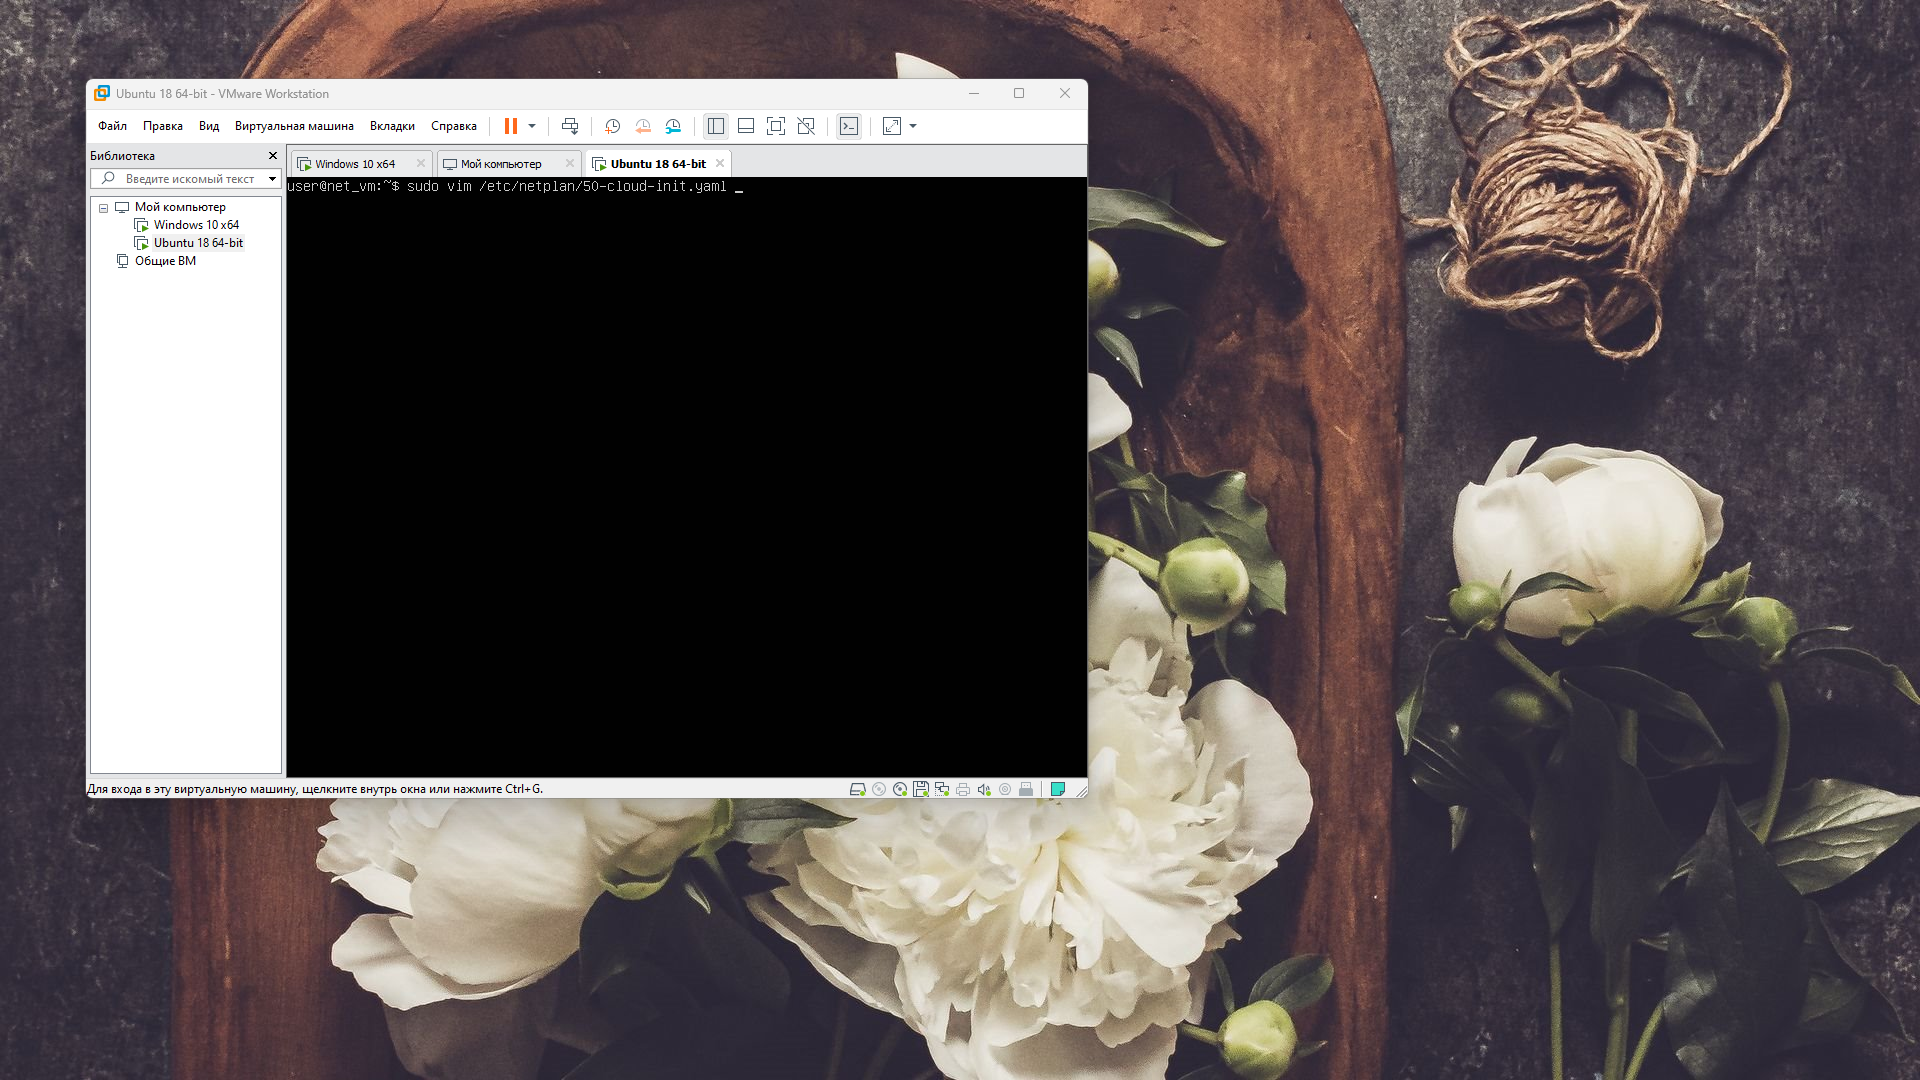
\includegraphics[width=0.85\textwidth]{06_00 (33)}
    \label{img:33}
    \caption{Открываем конфиг \textit{netplan} с помощью \textit{vim}}
  \end{figure}
  
  Настраиваем уже существующий сетевой интерфейс \textit{ens33}:
  указываем шлюз, \textit{DNS}, адрес устройства (для данной машины я выбрал
  10.15.10.6) и маску, а также режим \textit{DHCP} - отключен:
  
  \begin{figure}[H]
    \centering
    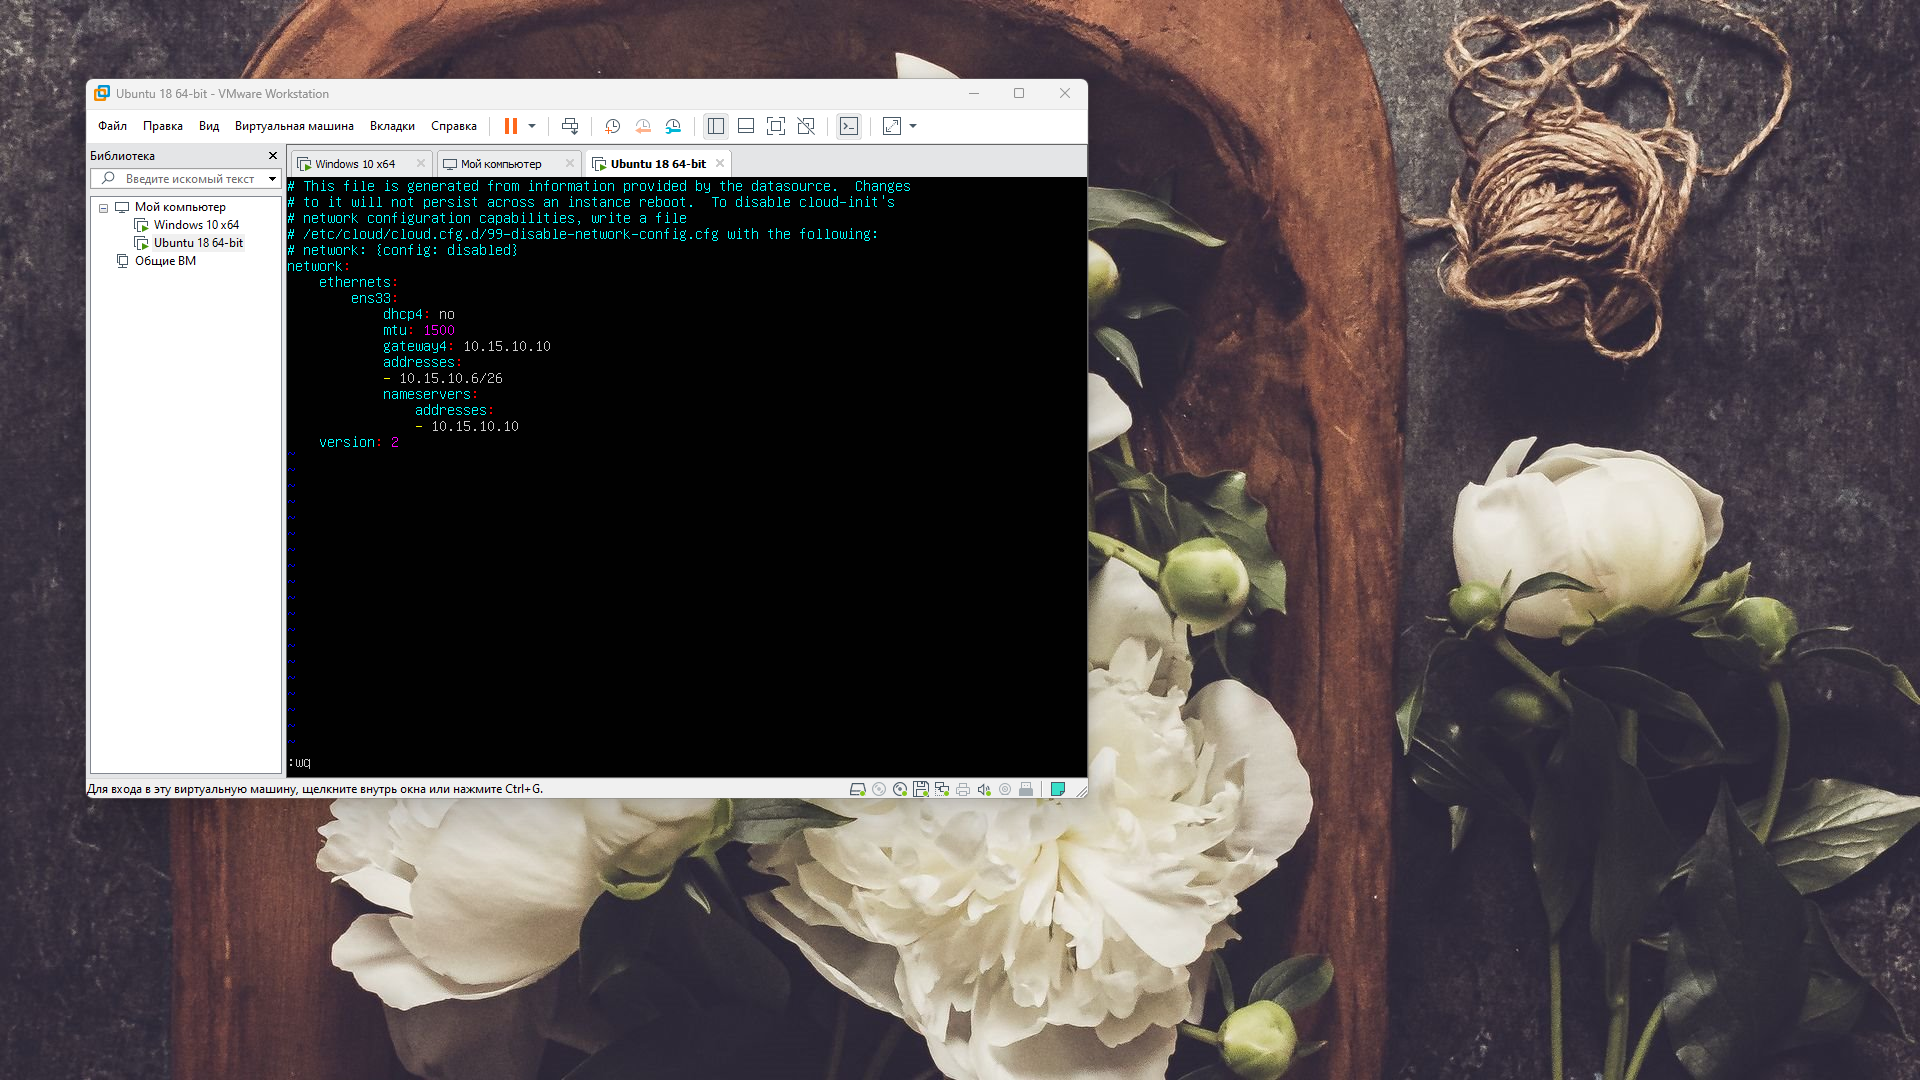
\includegraphics[width=0.85\textwidth]{06_00 (35)}
    \label{img:35}
    \caption{Получившийся конфиг}
  \end{figure}
  
  Сохраняем файл с настройками и выполняем его проверку на корректность:

  \begin{figure}[H]
    \centering
    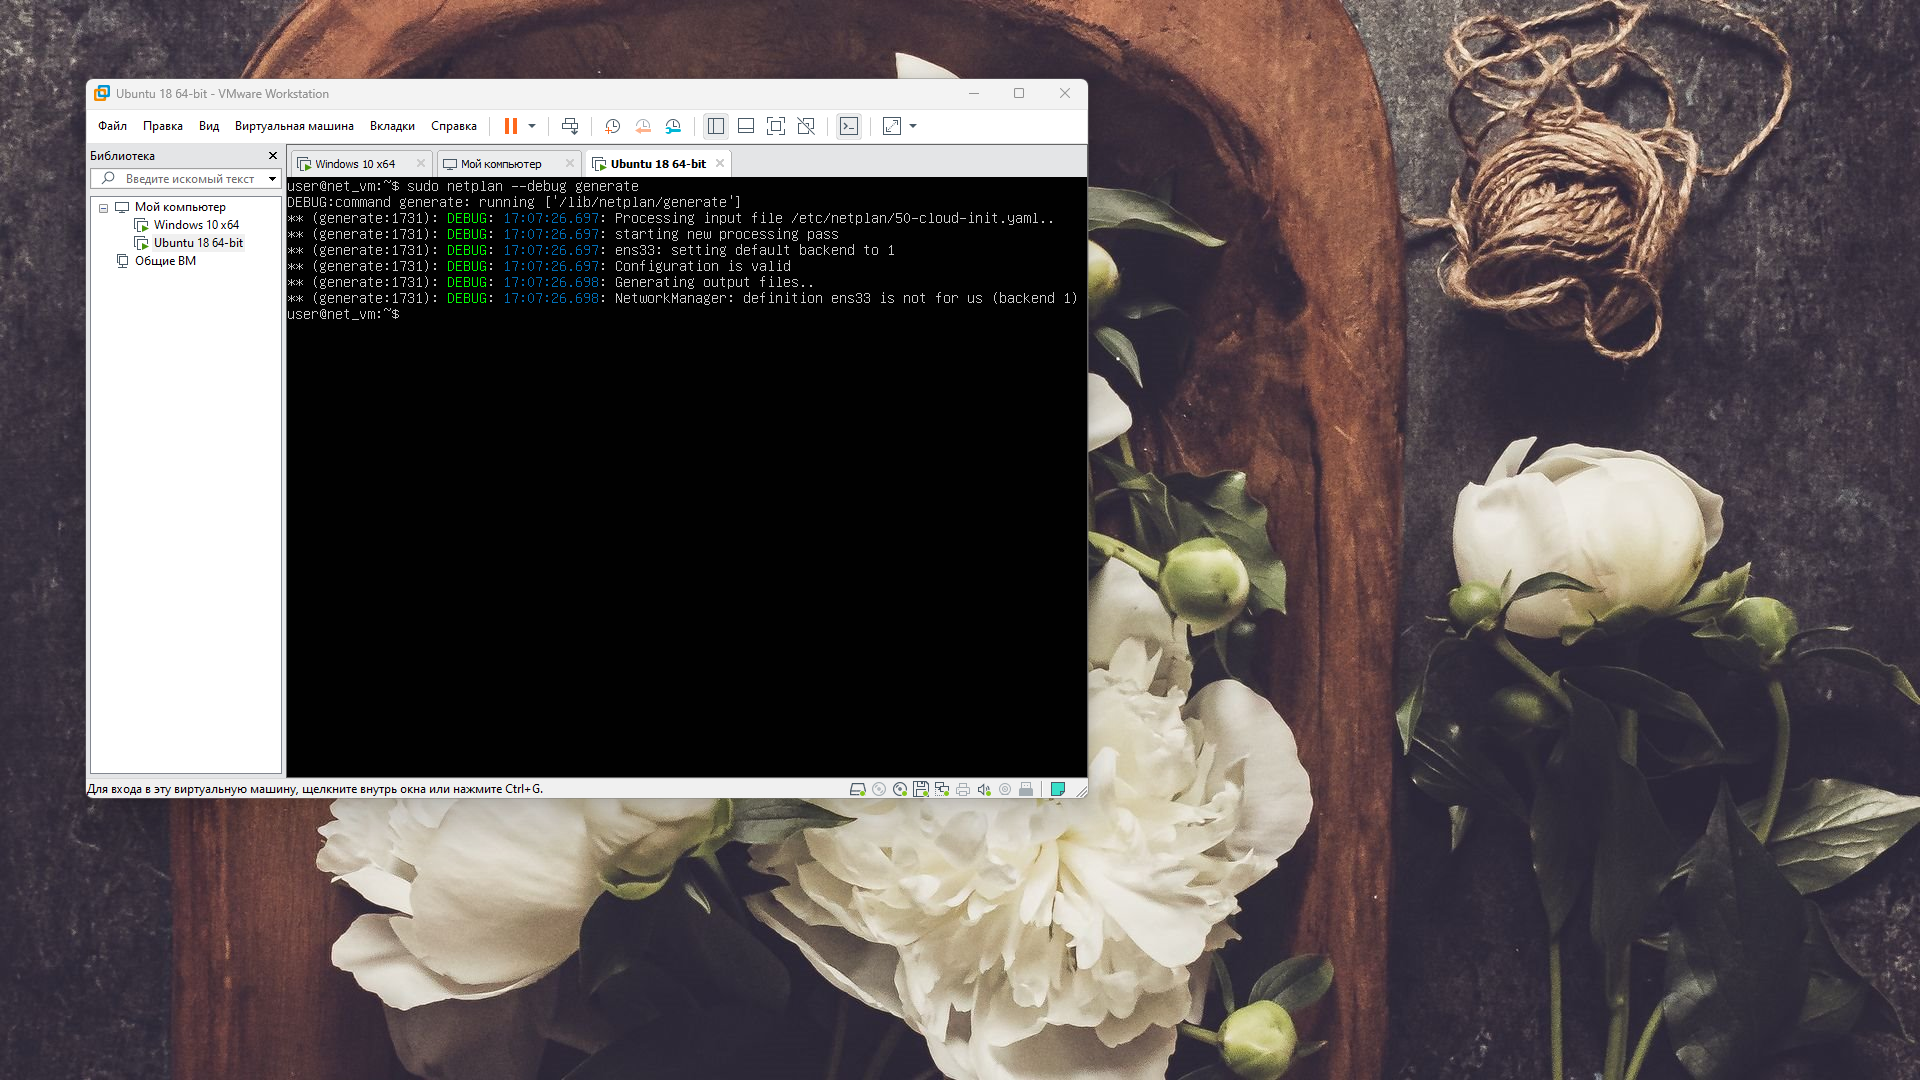
\includegraphics[width=0.85\textwidth]{06_00 (36)}
    \label{img:36}
    \caption{netplan generate - проверка конфига на валидность}
  \end{figure}
  
  Все настроенно верно - применяем данную конфигурацию:

  \begin{figure}[H]
    \centering
    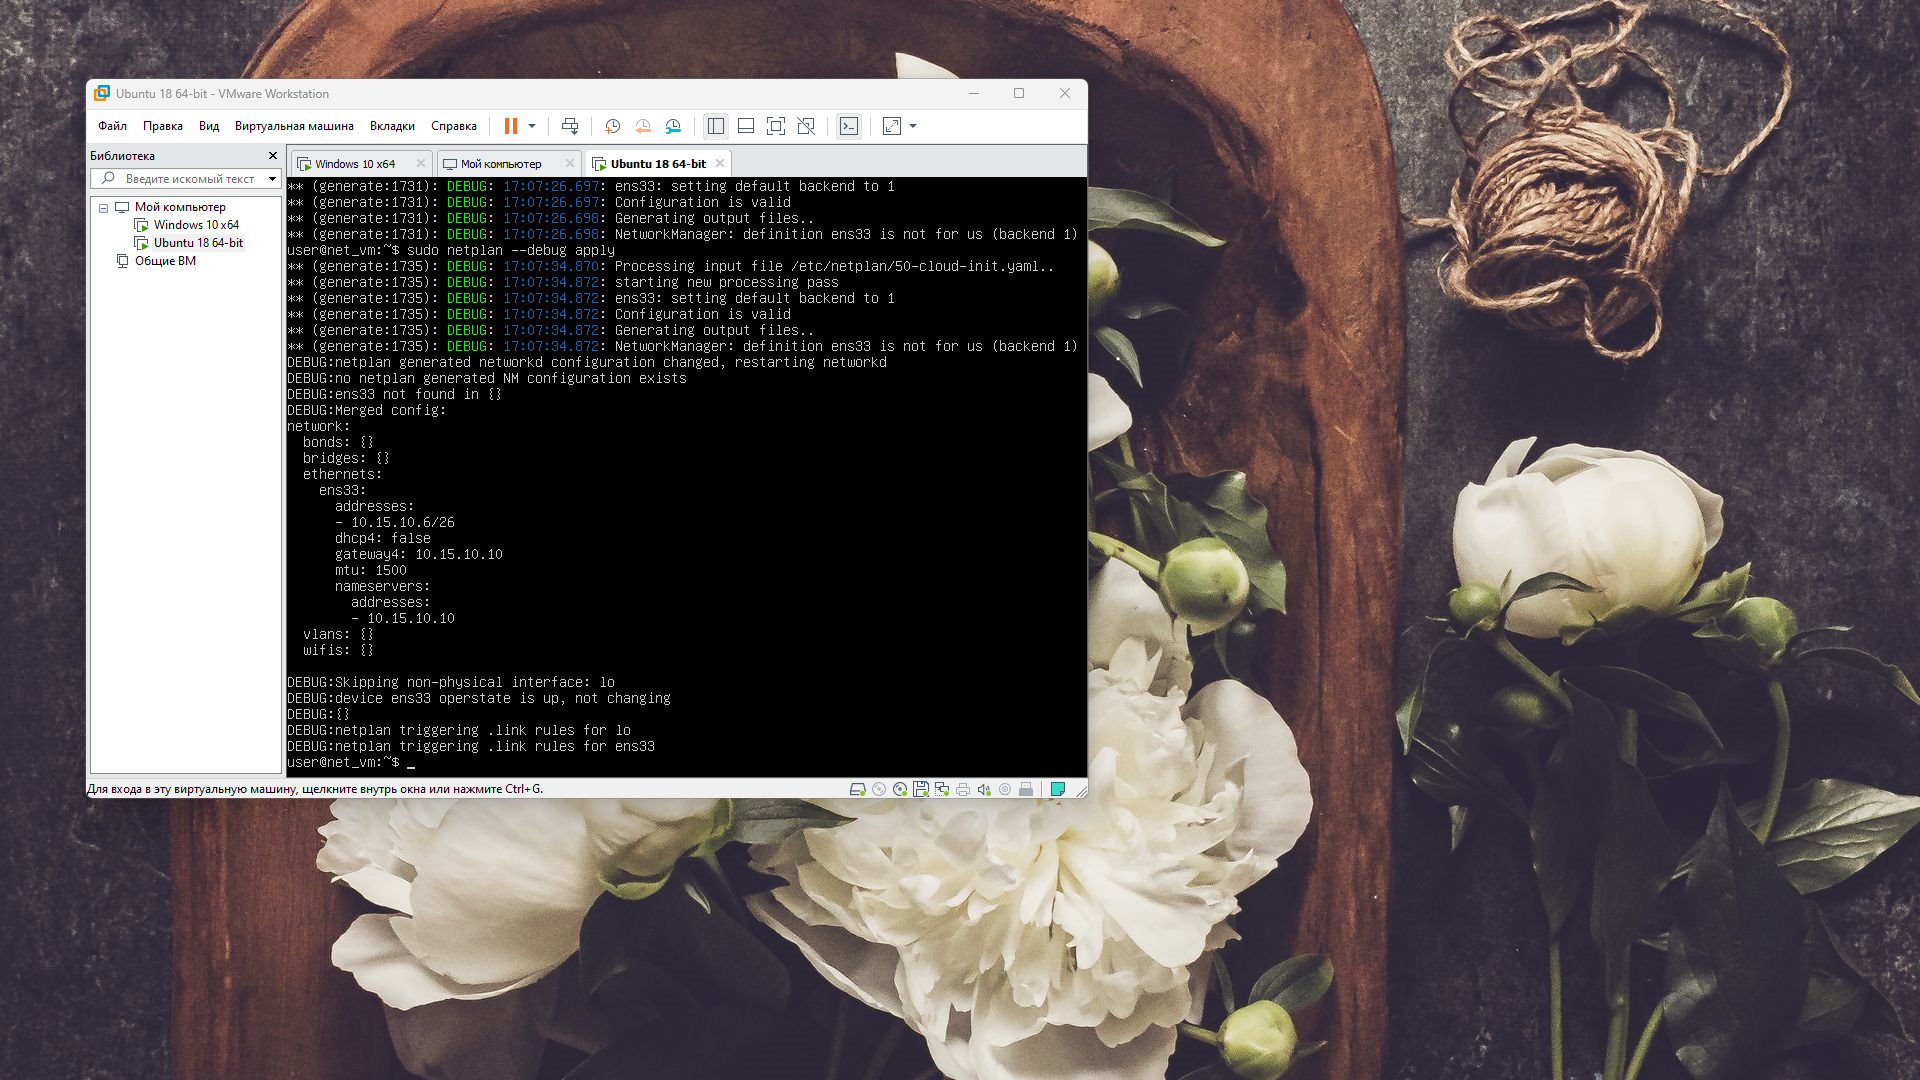
\includegraphics[width=0.85\textwidth]{06_00 (37)}
    \label{img:37}
    \caption{netplan apply - применение изменений}
  \end{figure}
  
  Проверим, вступили ли изменения в силу при помощи утилиты \textit{ip}:

  \begin{figure}[H]
    \centering
    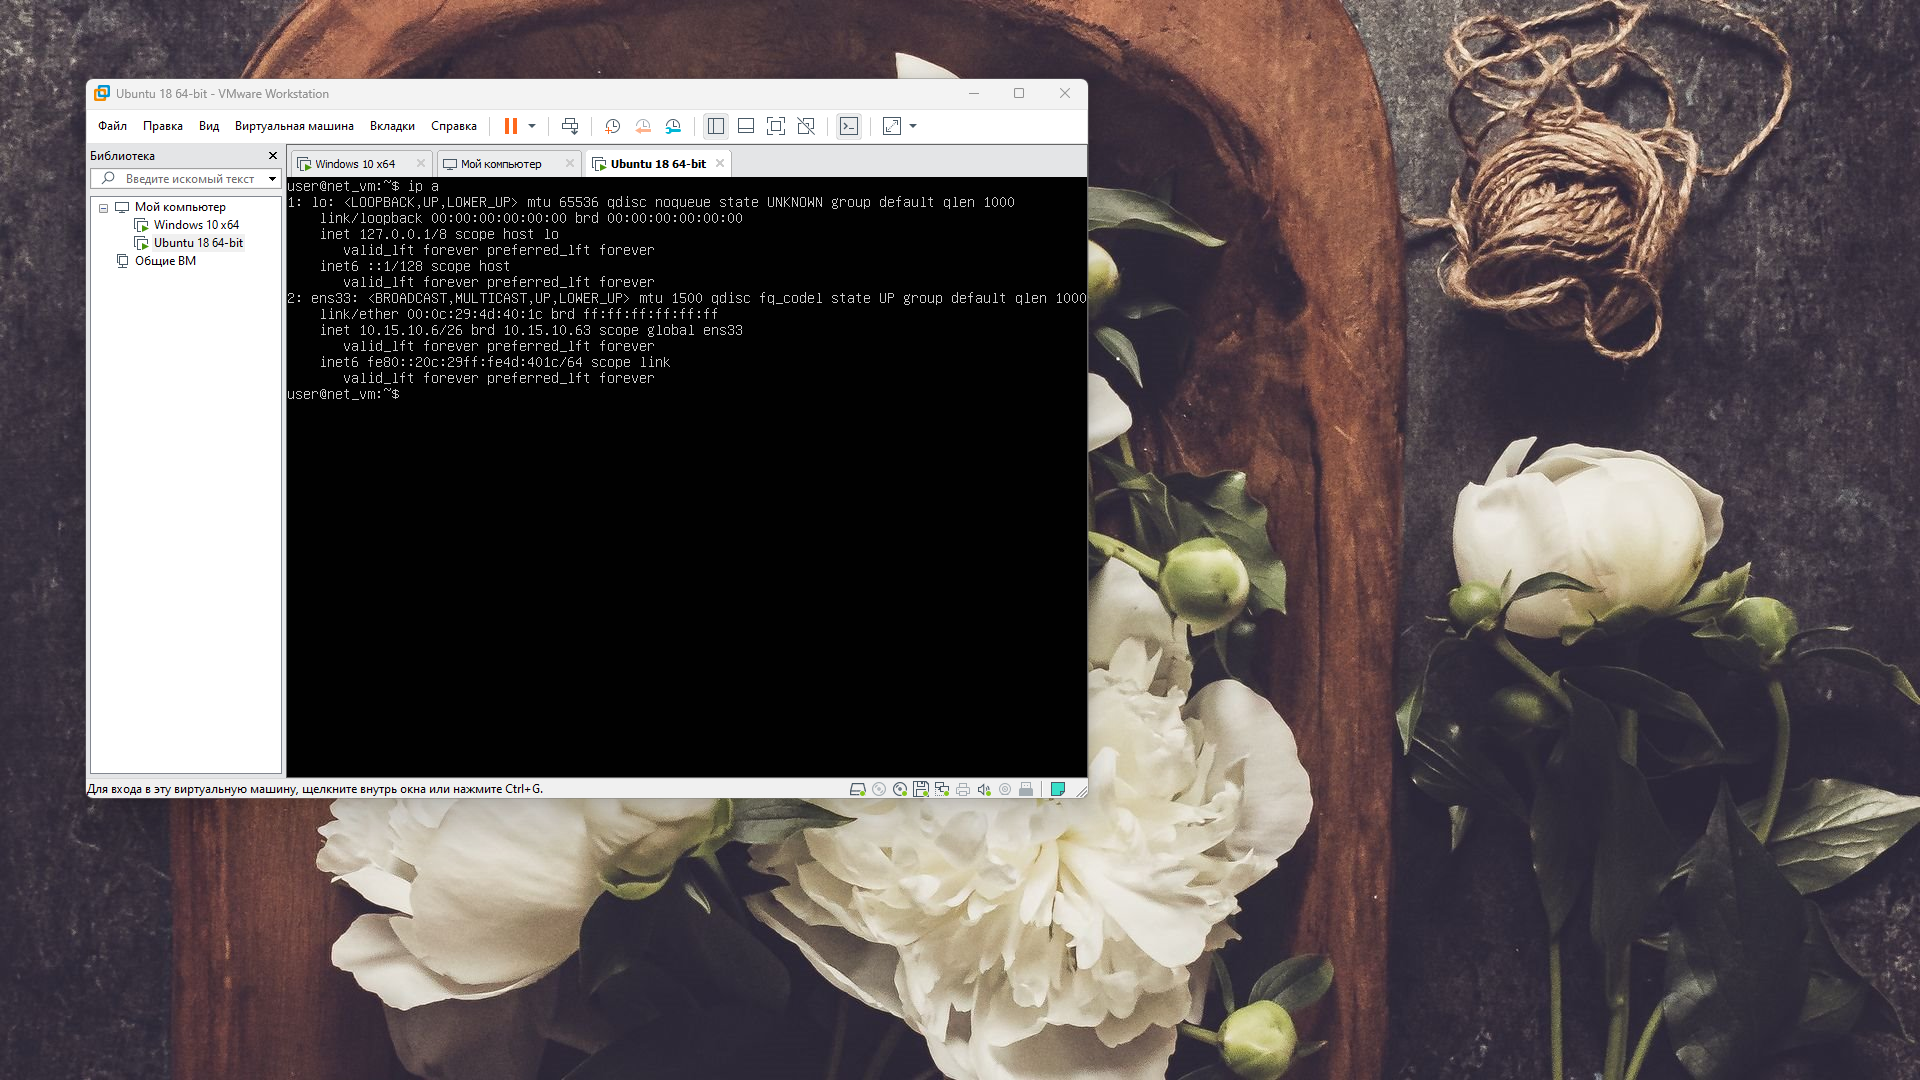
\includegraphics[width=0.85\textwidth]{06_00 (38)}
    \label{img:38}
    \caption{ip a - информация о всех сетевых интерфейсах}
  \end{figure}
  
  Как видно, для интерфейса \textit{ens33} установлен правильный \textit{IPv4} адрес и маска подсети.

  Также выполним проверку, что данная машина имеет доступ в Интернет и может достучаться до шлюза по умолчанию:

  \begin{figure}[H]
    \centering
    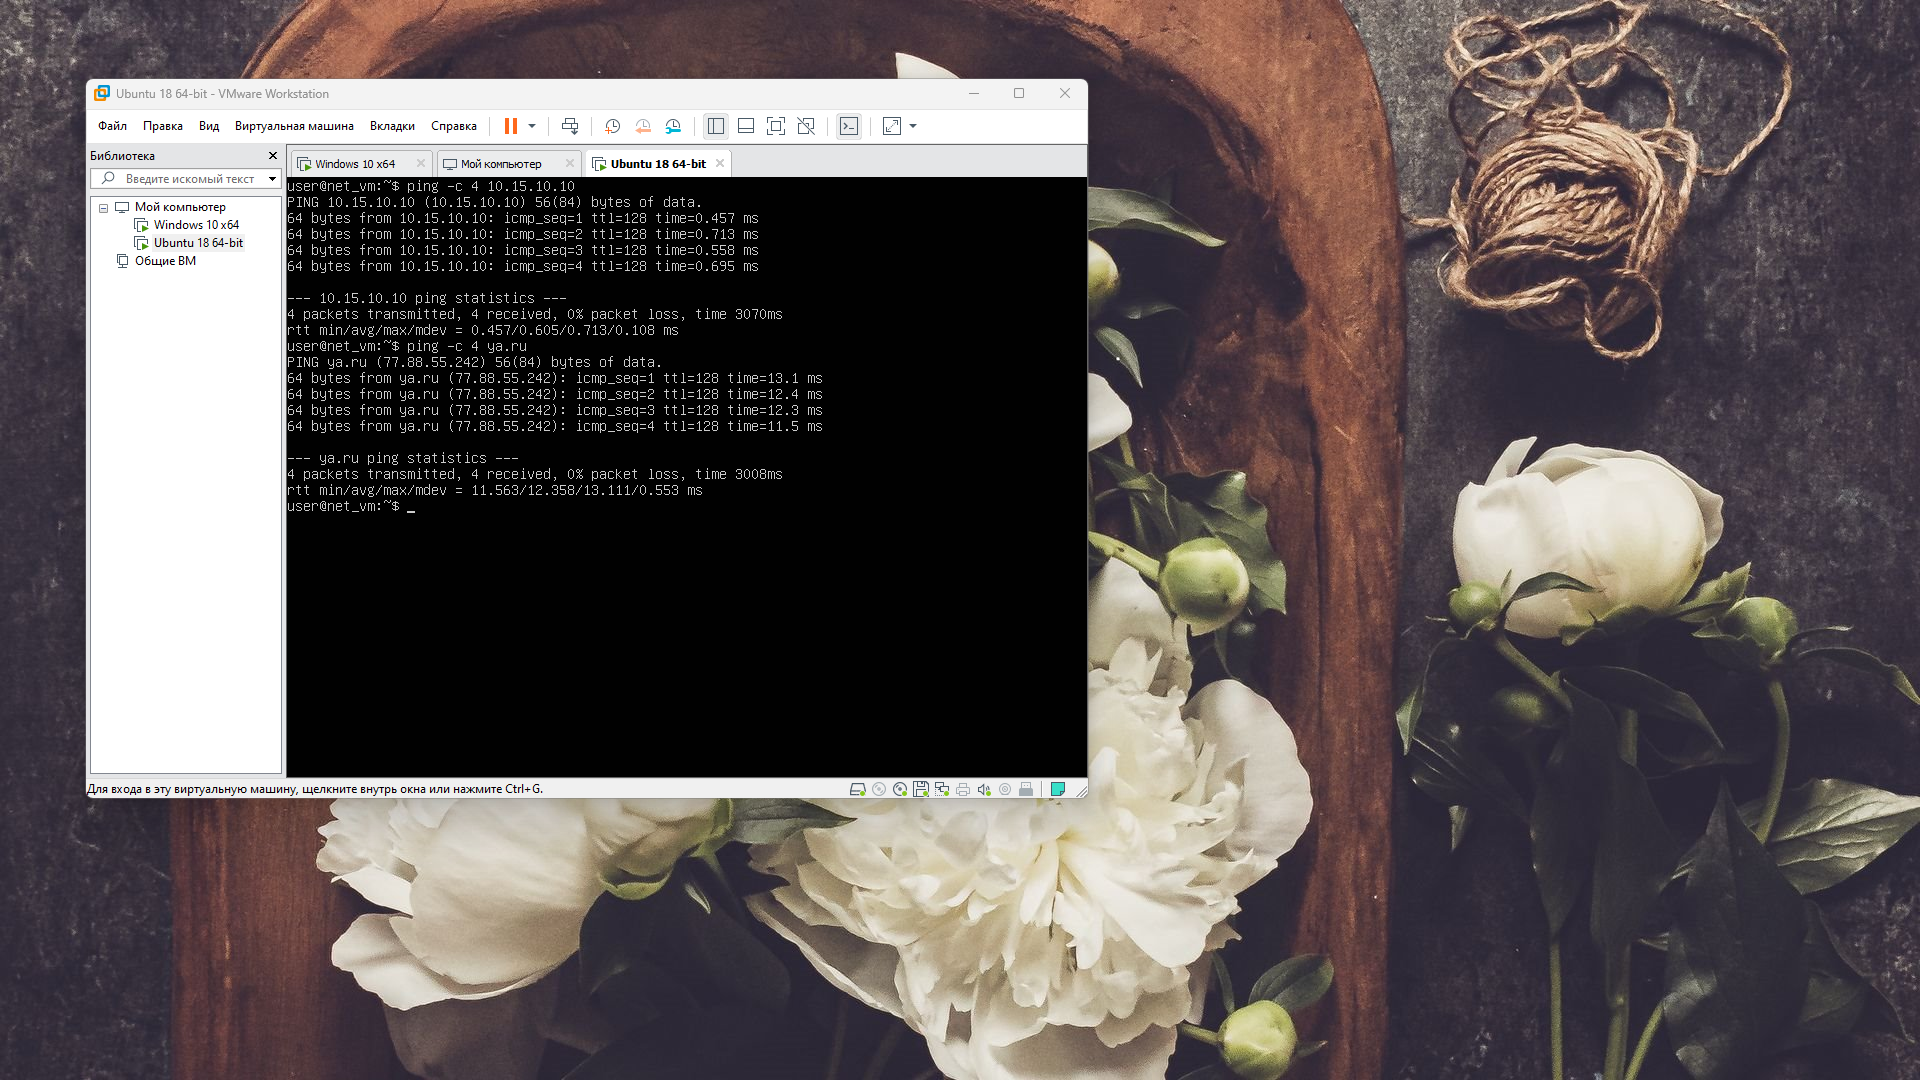
\includegraphics[width=0.85\textwidth]{06_00 (39)}
    \label{img:39}
    \caption{Проверка доступности}
  \end{figure}
  
  \subsubsection{Настройка Host-Only сети}

  Далее попробуем ностроить \textit{Host-Only} сеть без выхода в Интернет:

  \begin{figure}[H]
    \centering
    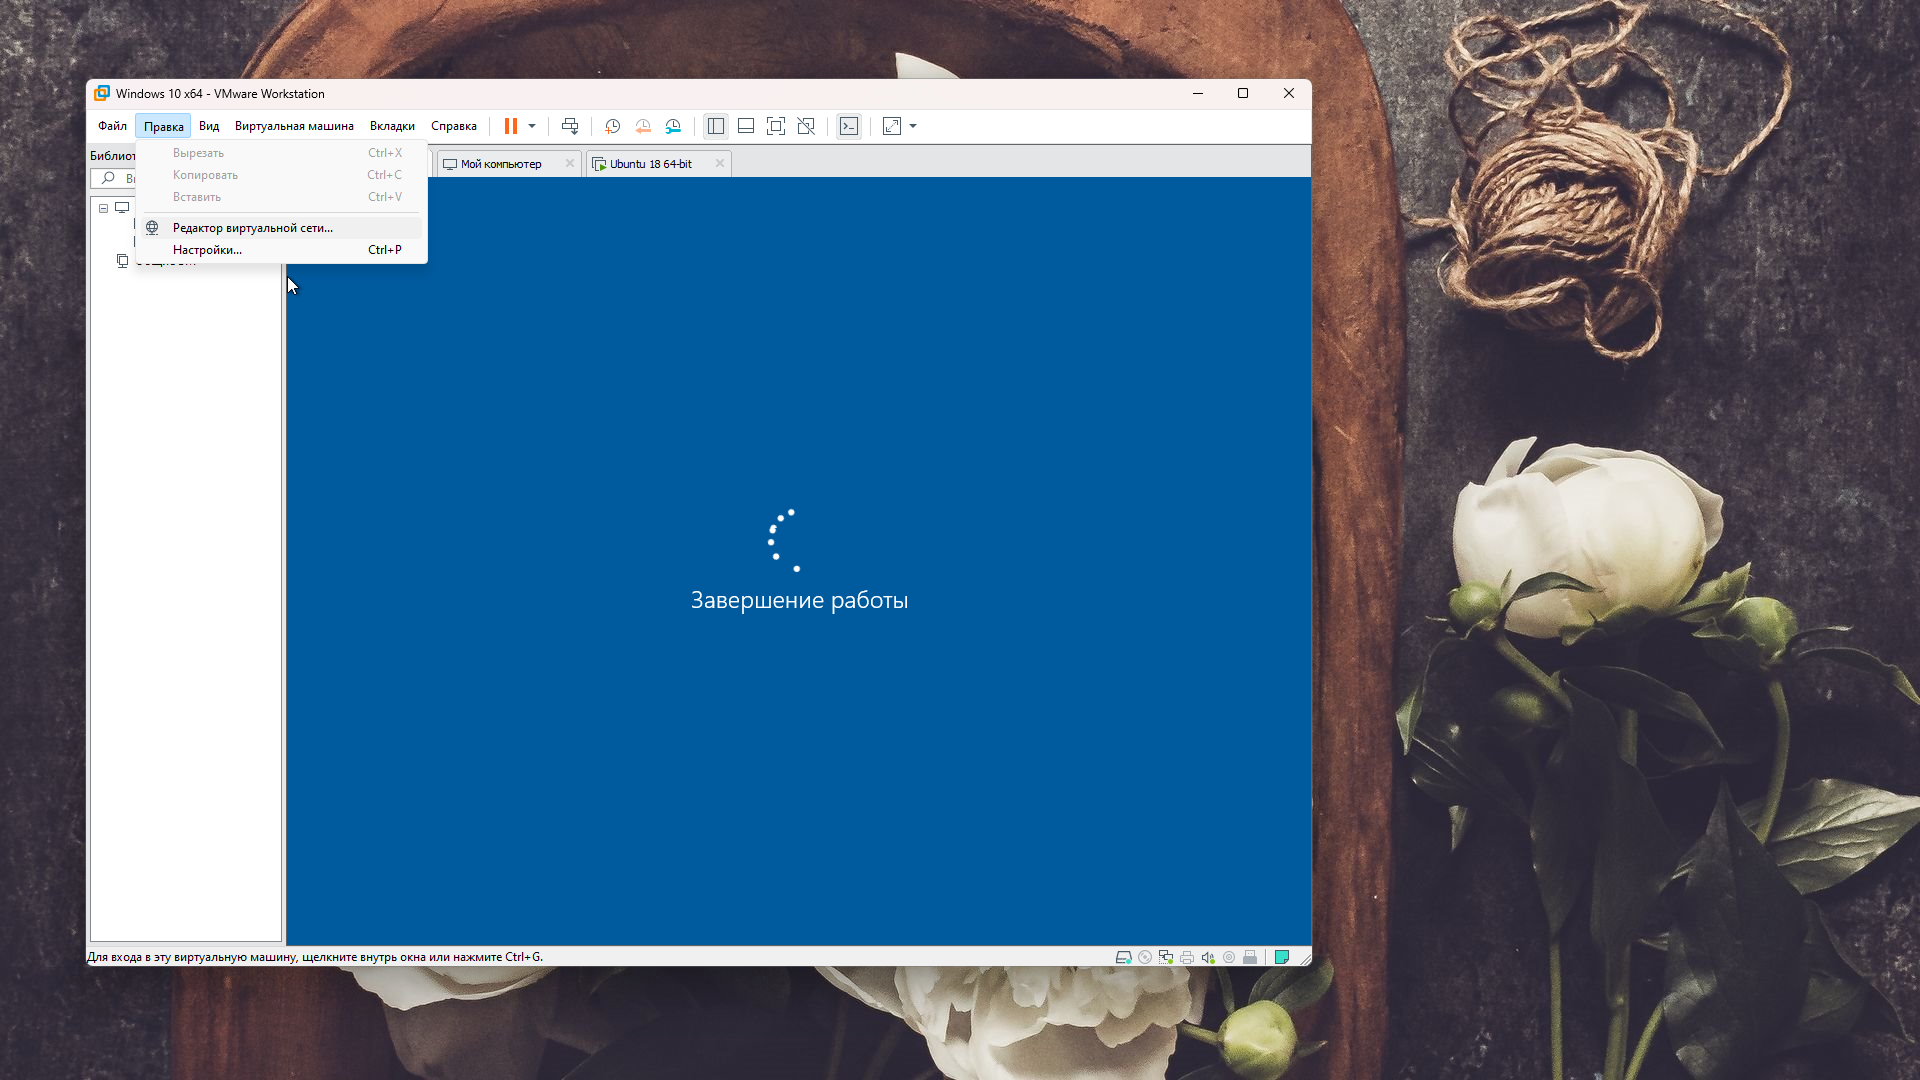
\includegraphics[width=0.85\textwidth]{06_00 (40)}
    \label{img:40}
    \caption{Снова открываем редактор виртульной сети}
  \end{figure}
  
  \begin{figure}[H]
    \centering
    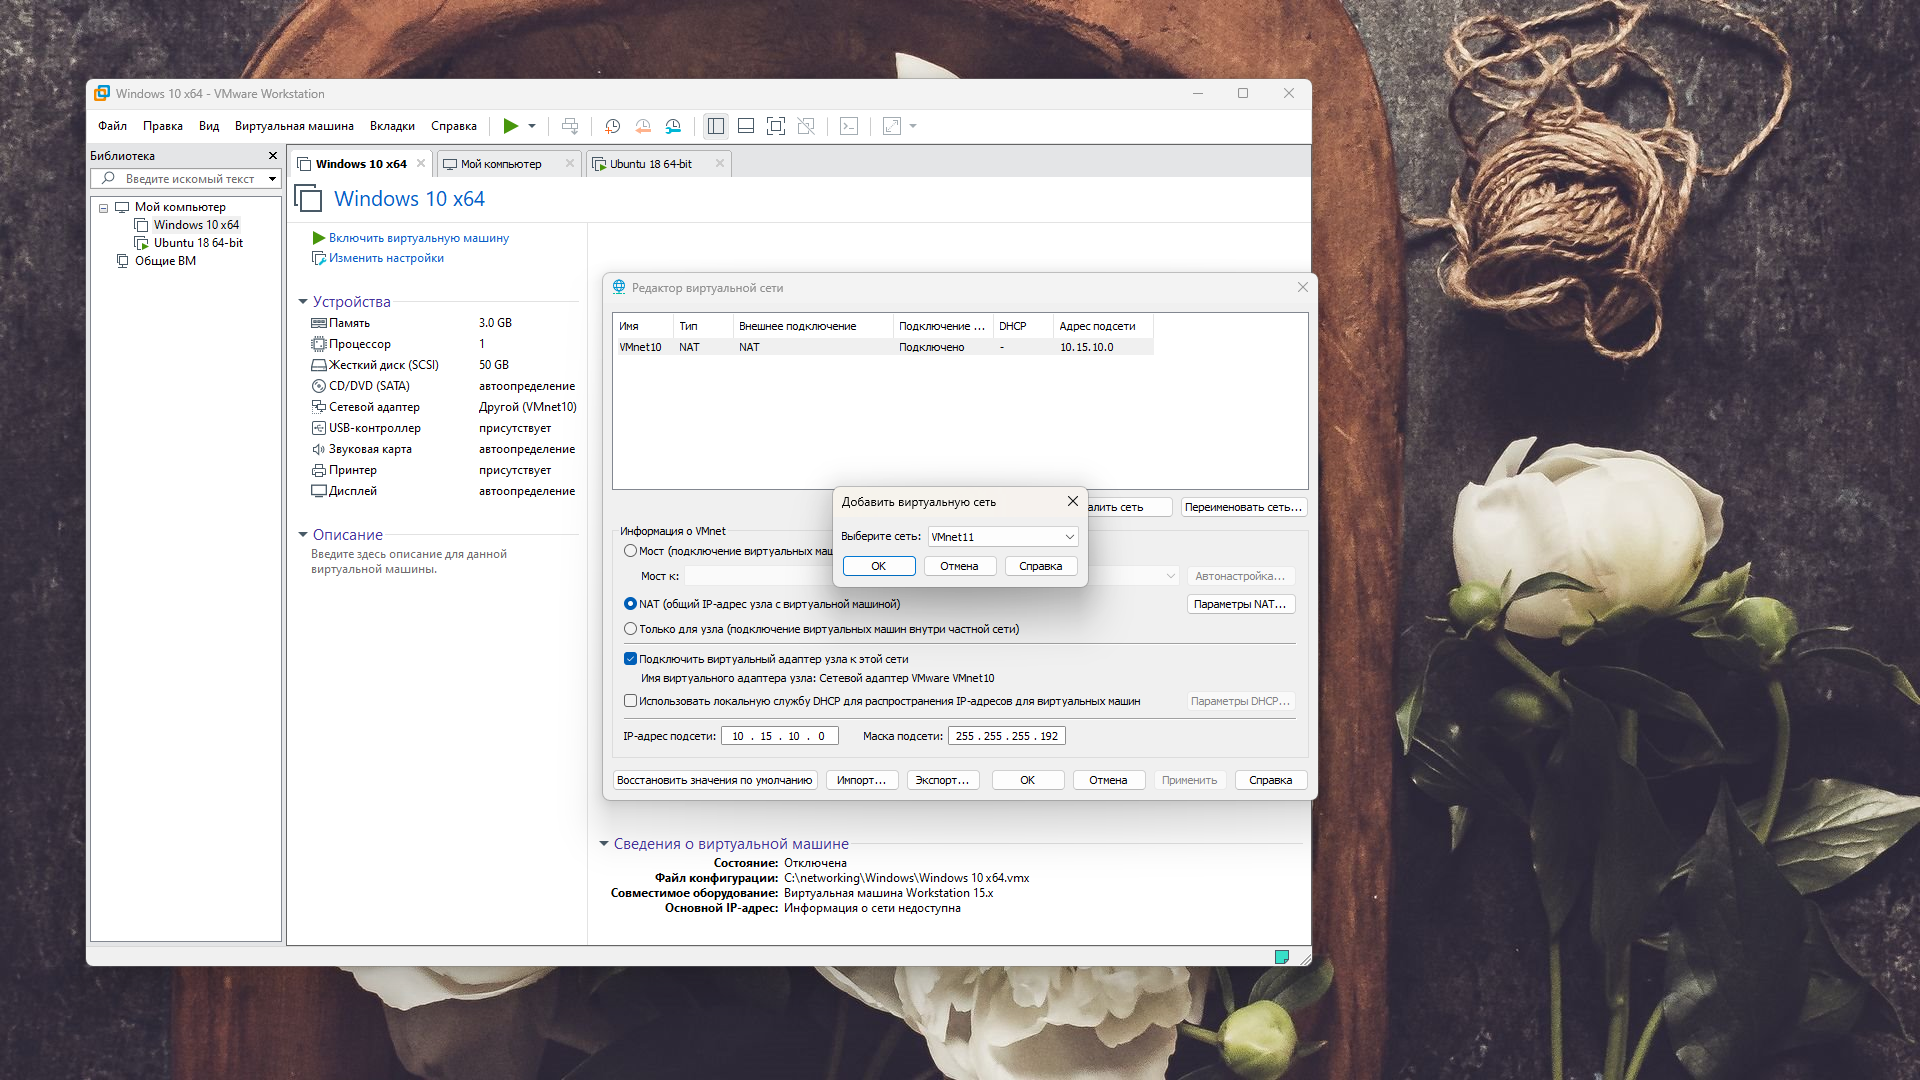
\includegraphics[width=0.85\textwidth]{06_00 (41)}
    \label{img:41}
    \caption{Создаем новую сеть и указываем ее имя}
  \end{figure}

  Для данной сети в 9 варианте указаны адрес 192.168.9.0 и маска 255.255.255.224 -
  устанавливаем их, также отключаем встроенный \textit{DHCP} сервер:
  
  \begin{figure}[H]
    \centering
    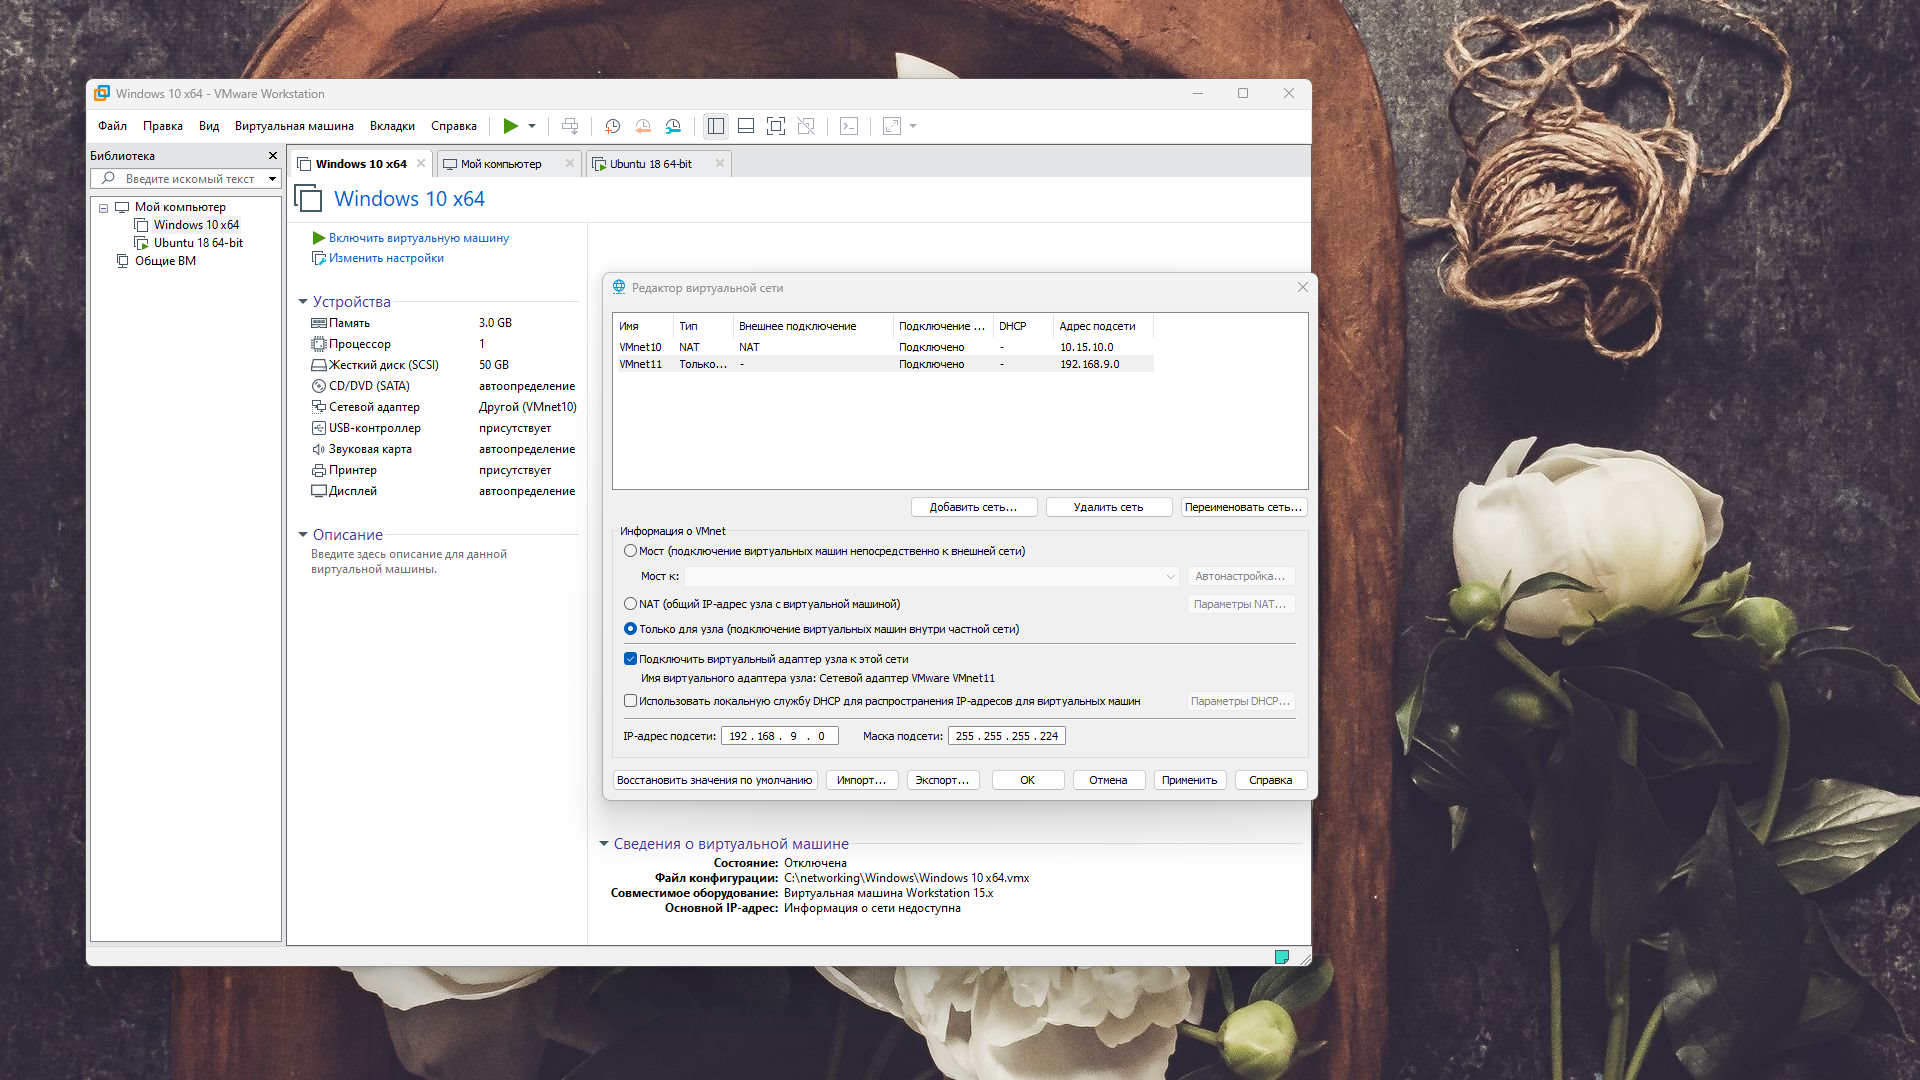
\includegraphics[width=0.85\textwidth]{06_00 (42)}
    \label{img:42}
    \caption{Настроенная сеть}
  \end{figure}
  
  Хостовая машина также имеет доступ к этой сети, поэтому сначала настроим ее:

  \begin{figure}[H]
    \centering
    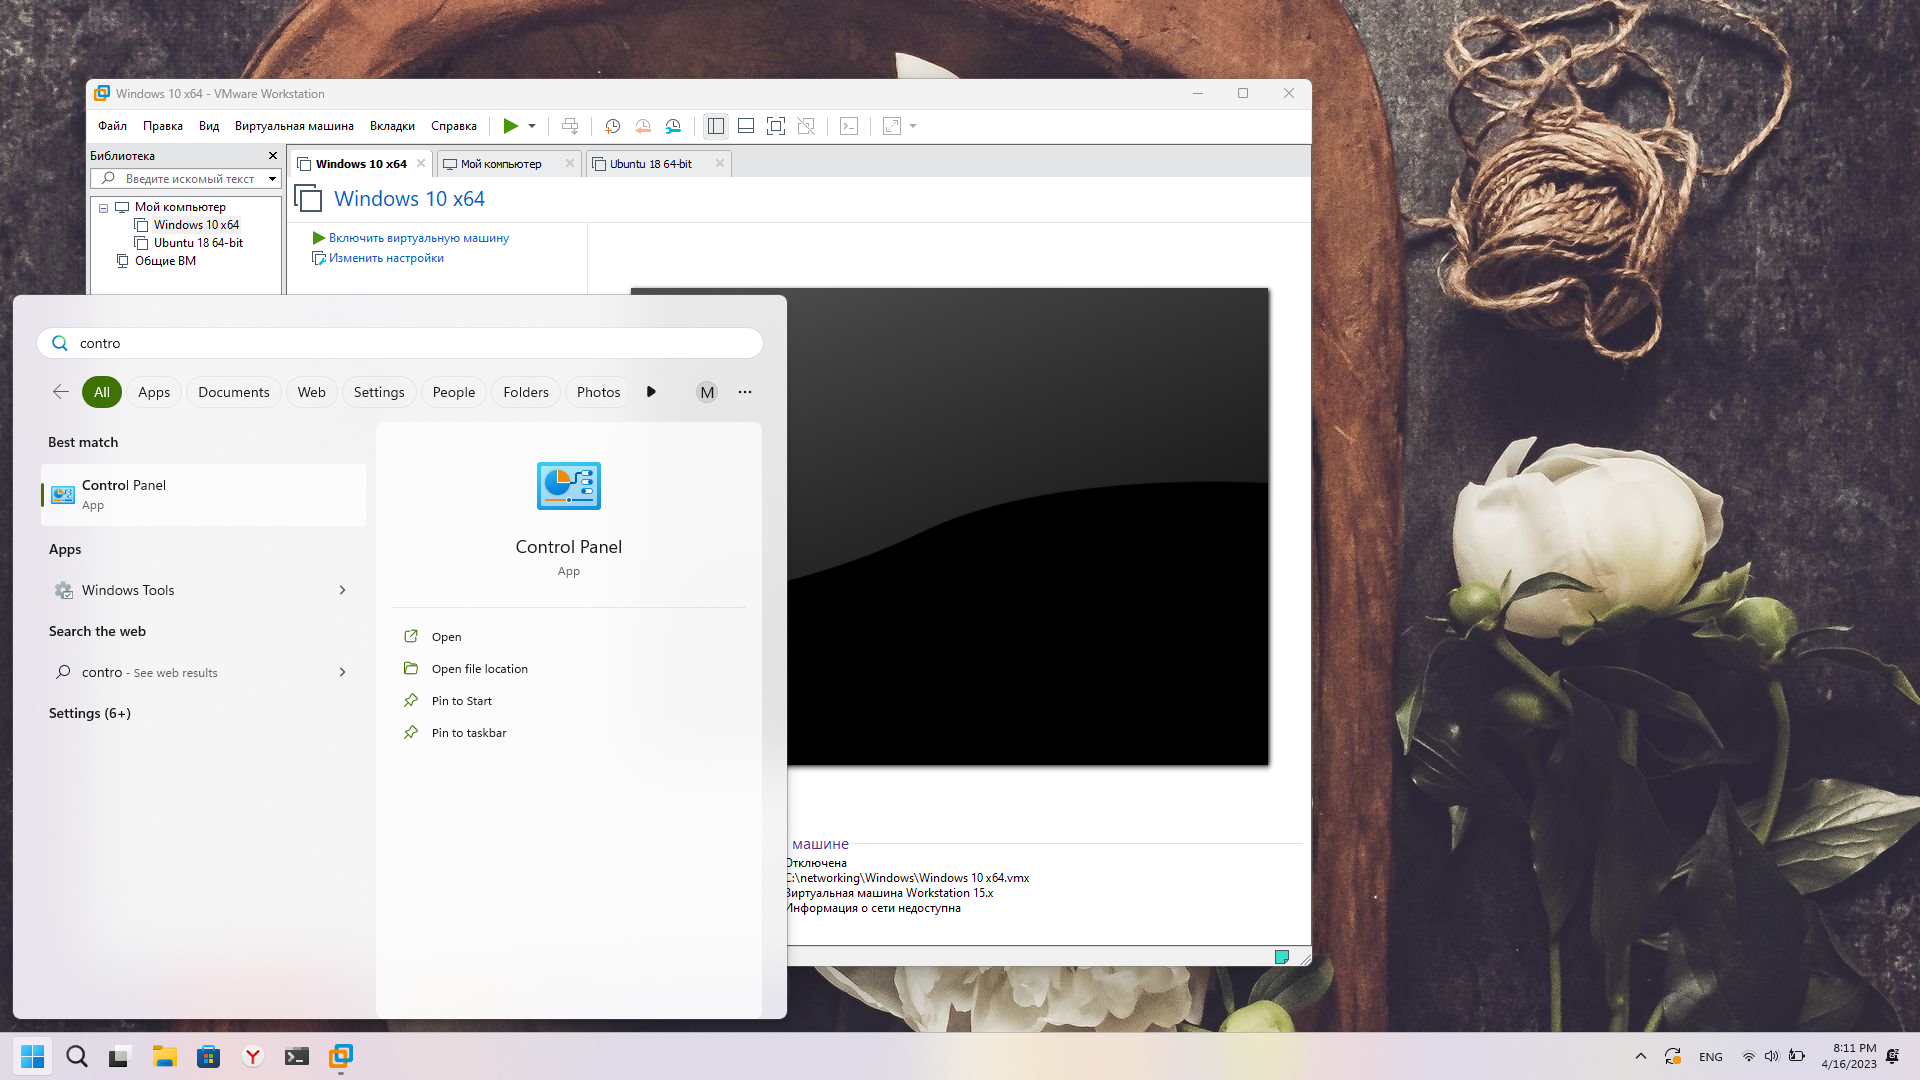
\includegraphics[width=0.85\textwidth]{06_00 (43)}
    \label{img:43}
    \caption{Открываем Панель Задач}
  \end{figure}
  
  \begin{figure}[H]
    \centering
    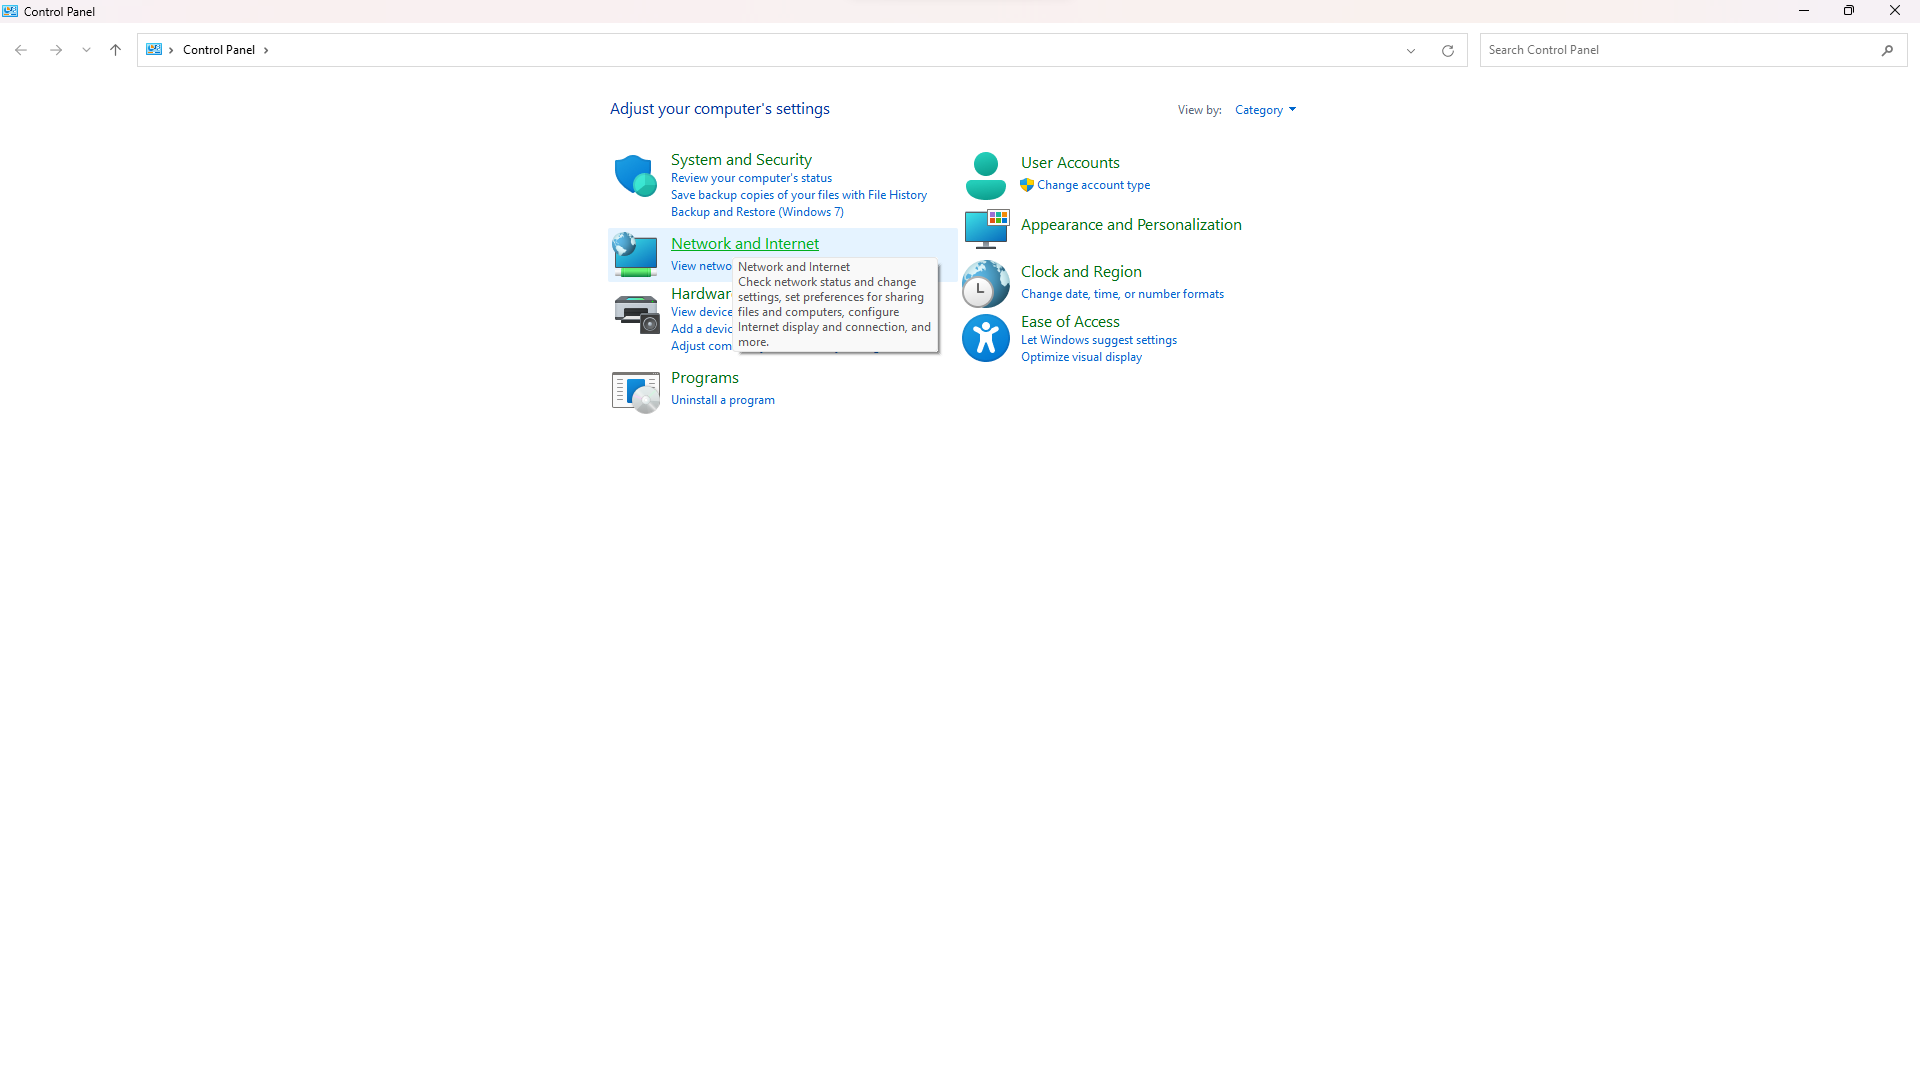
\includegraphics[width=0.85\textwidth]{06_00 (44)}
    \label{img:44}
    \caption{Открываем вкладку "Сеть и Интернет"}
  \end{figure}
  
  \begin{figure}[H]
    \centering
    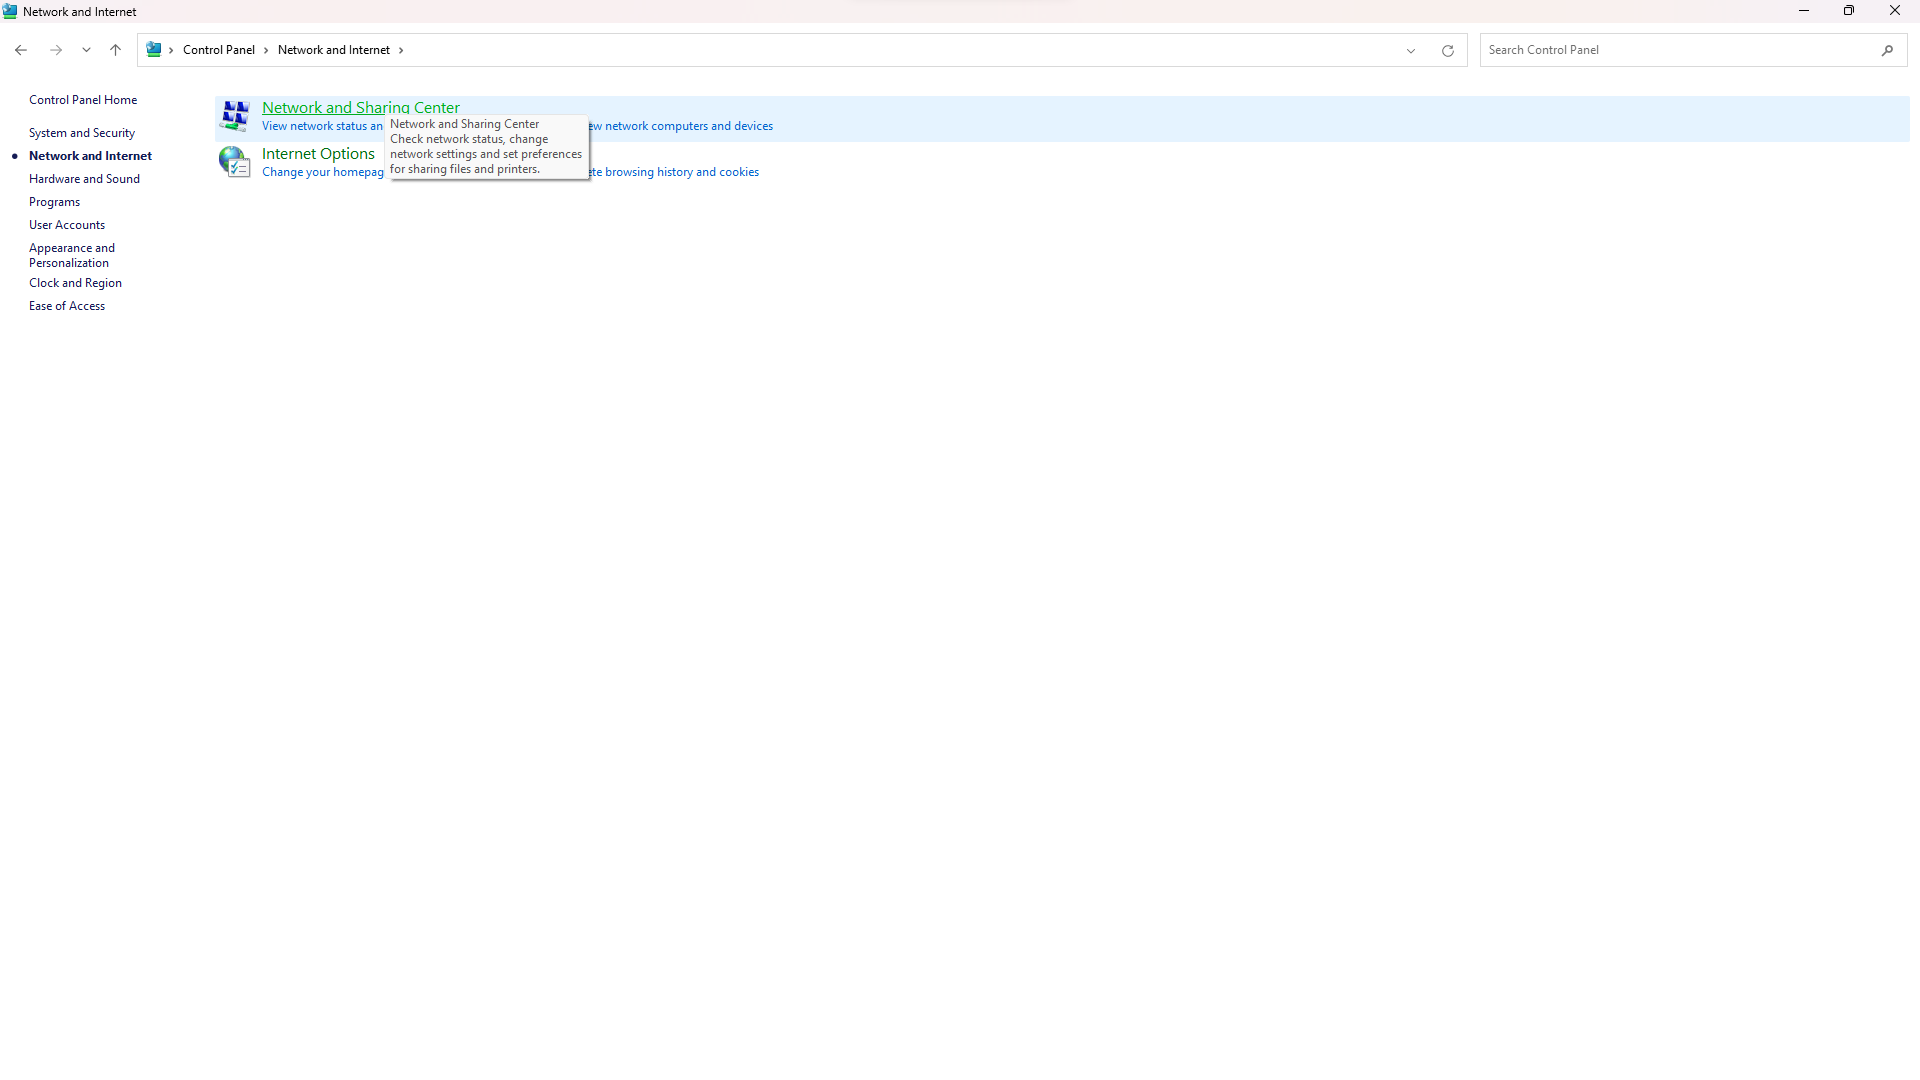
\includegraphics[width=0.85\textwidth]{06_00 (45)}
    \label{img:45}
    \caption{Параметры сети и общего доступа}
  \end{figure}
  
  \begin{figure}[H]
    \centering
    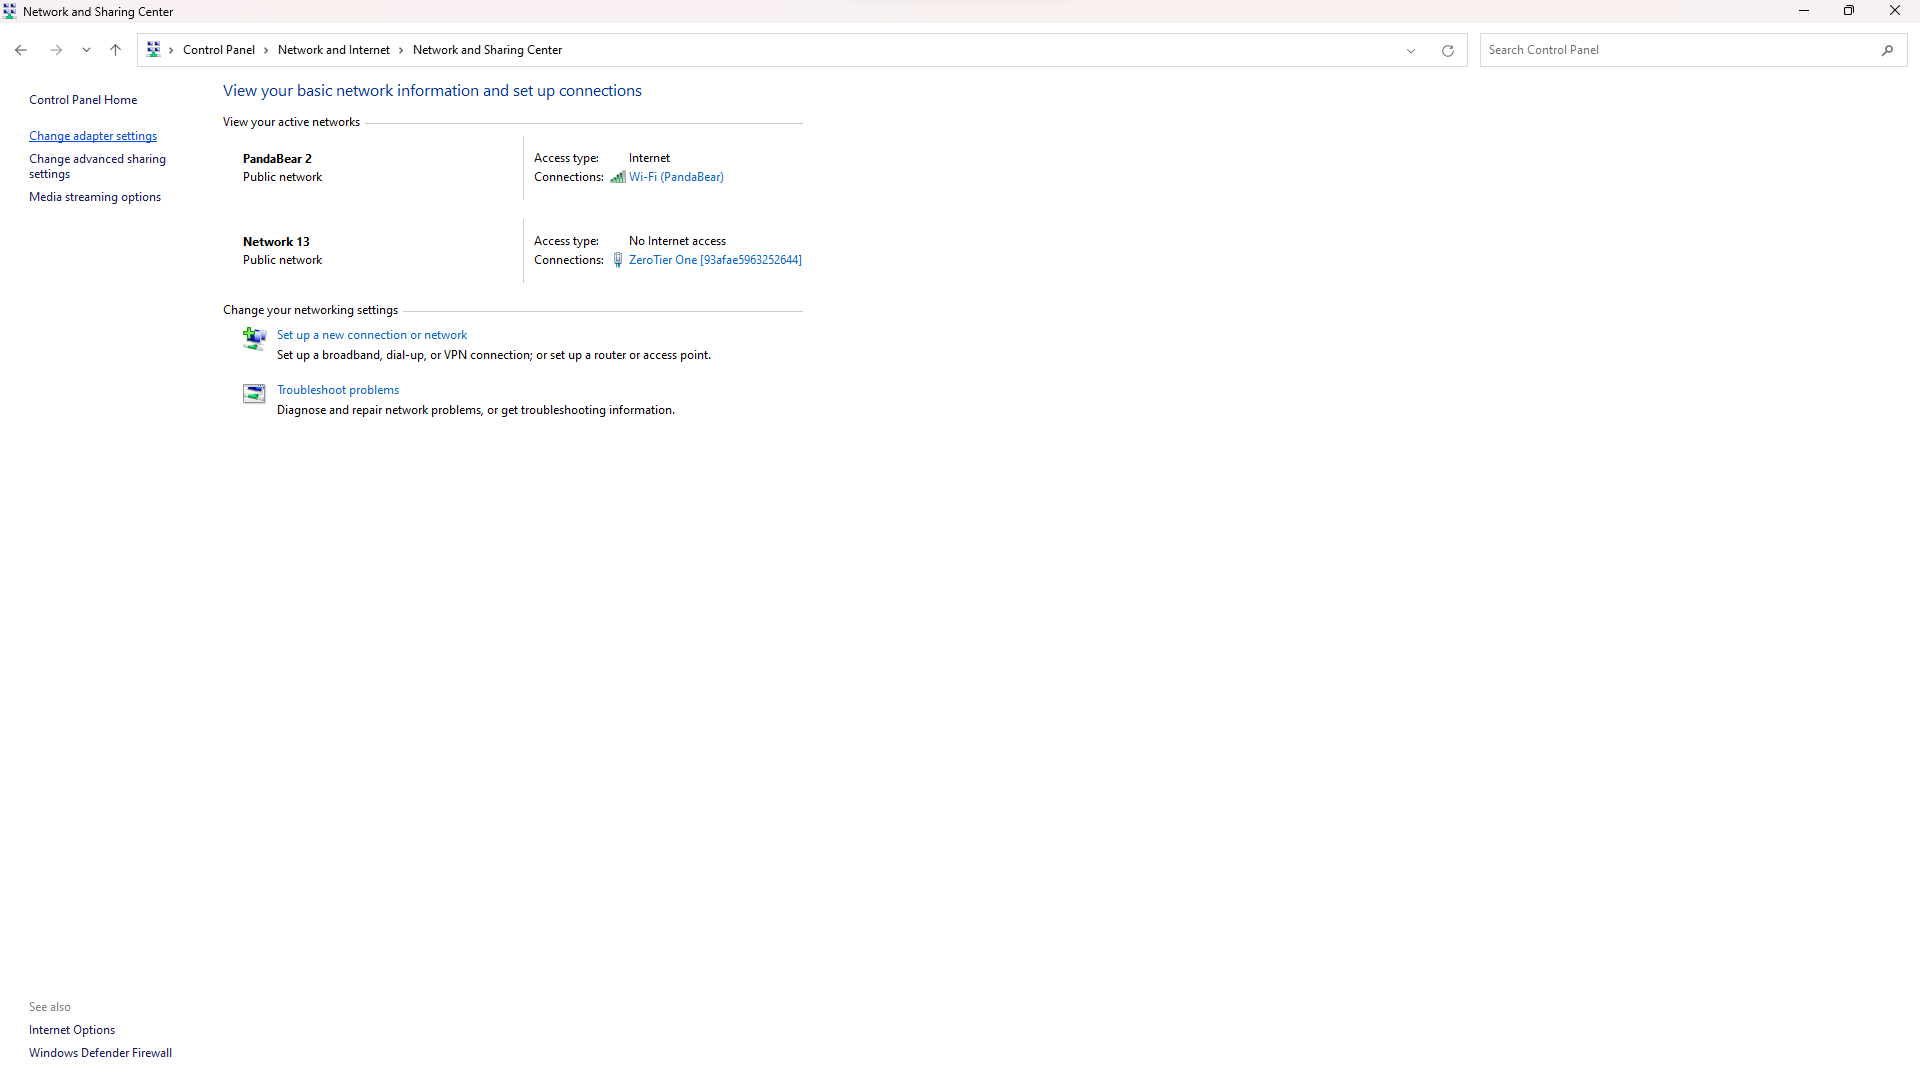
\includegraphics[width=0.85\textwidth]{06_00 (46)}
    \label{img:46}
    \caption{Выбираем пункт "Редактирование параметров адаптеров"}
  \end{figure}
  
  \begin{figure}[H]
    \centering
    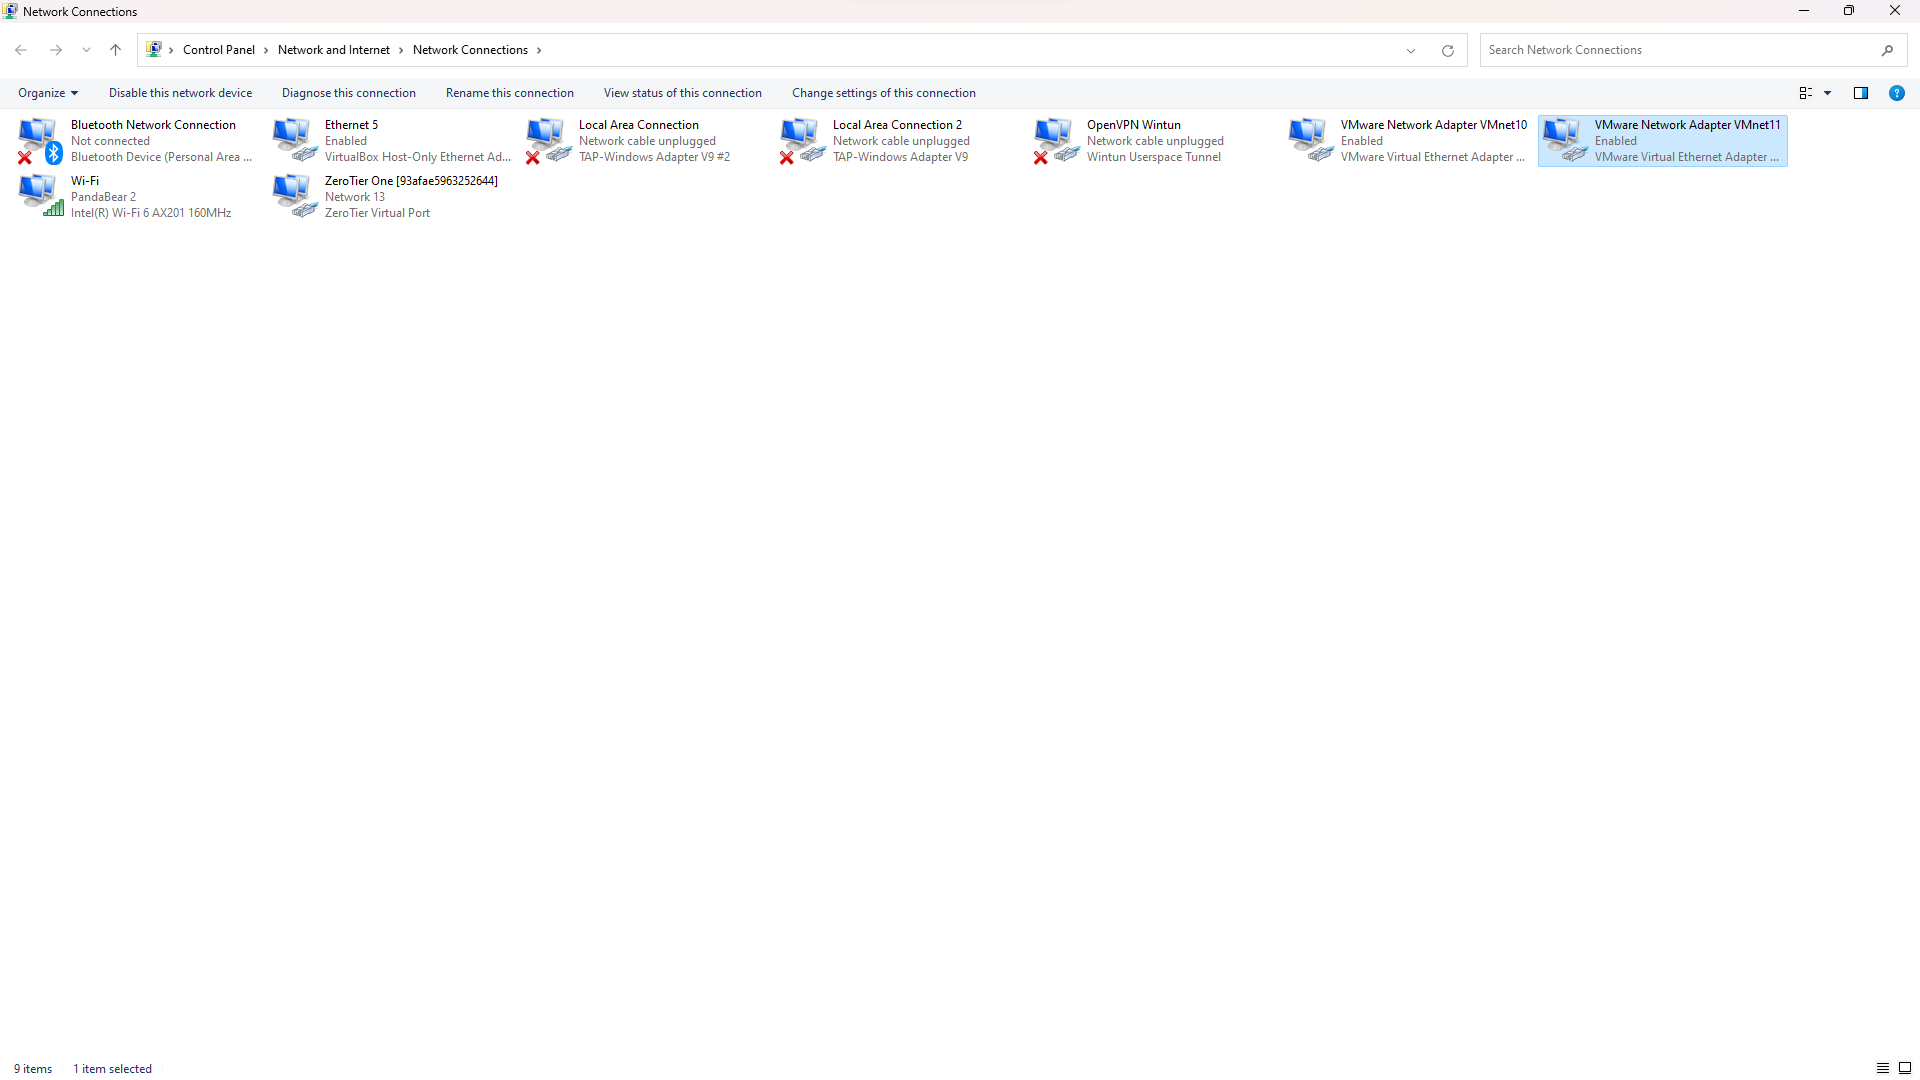
\includegraphics[width=0.85\textwidth]{06_00 (47)}
    \label{img:47}
    \caption{Открываем нужный адаптер - VMNet 11 (как имя сети)}
  \end{figure}
  
  \begin{figure}[H]
    \centering
    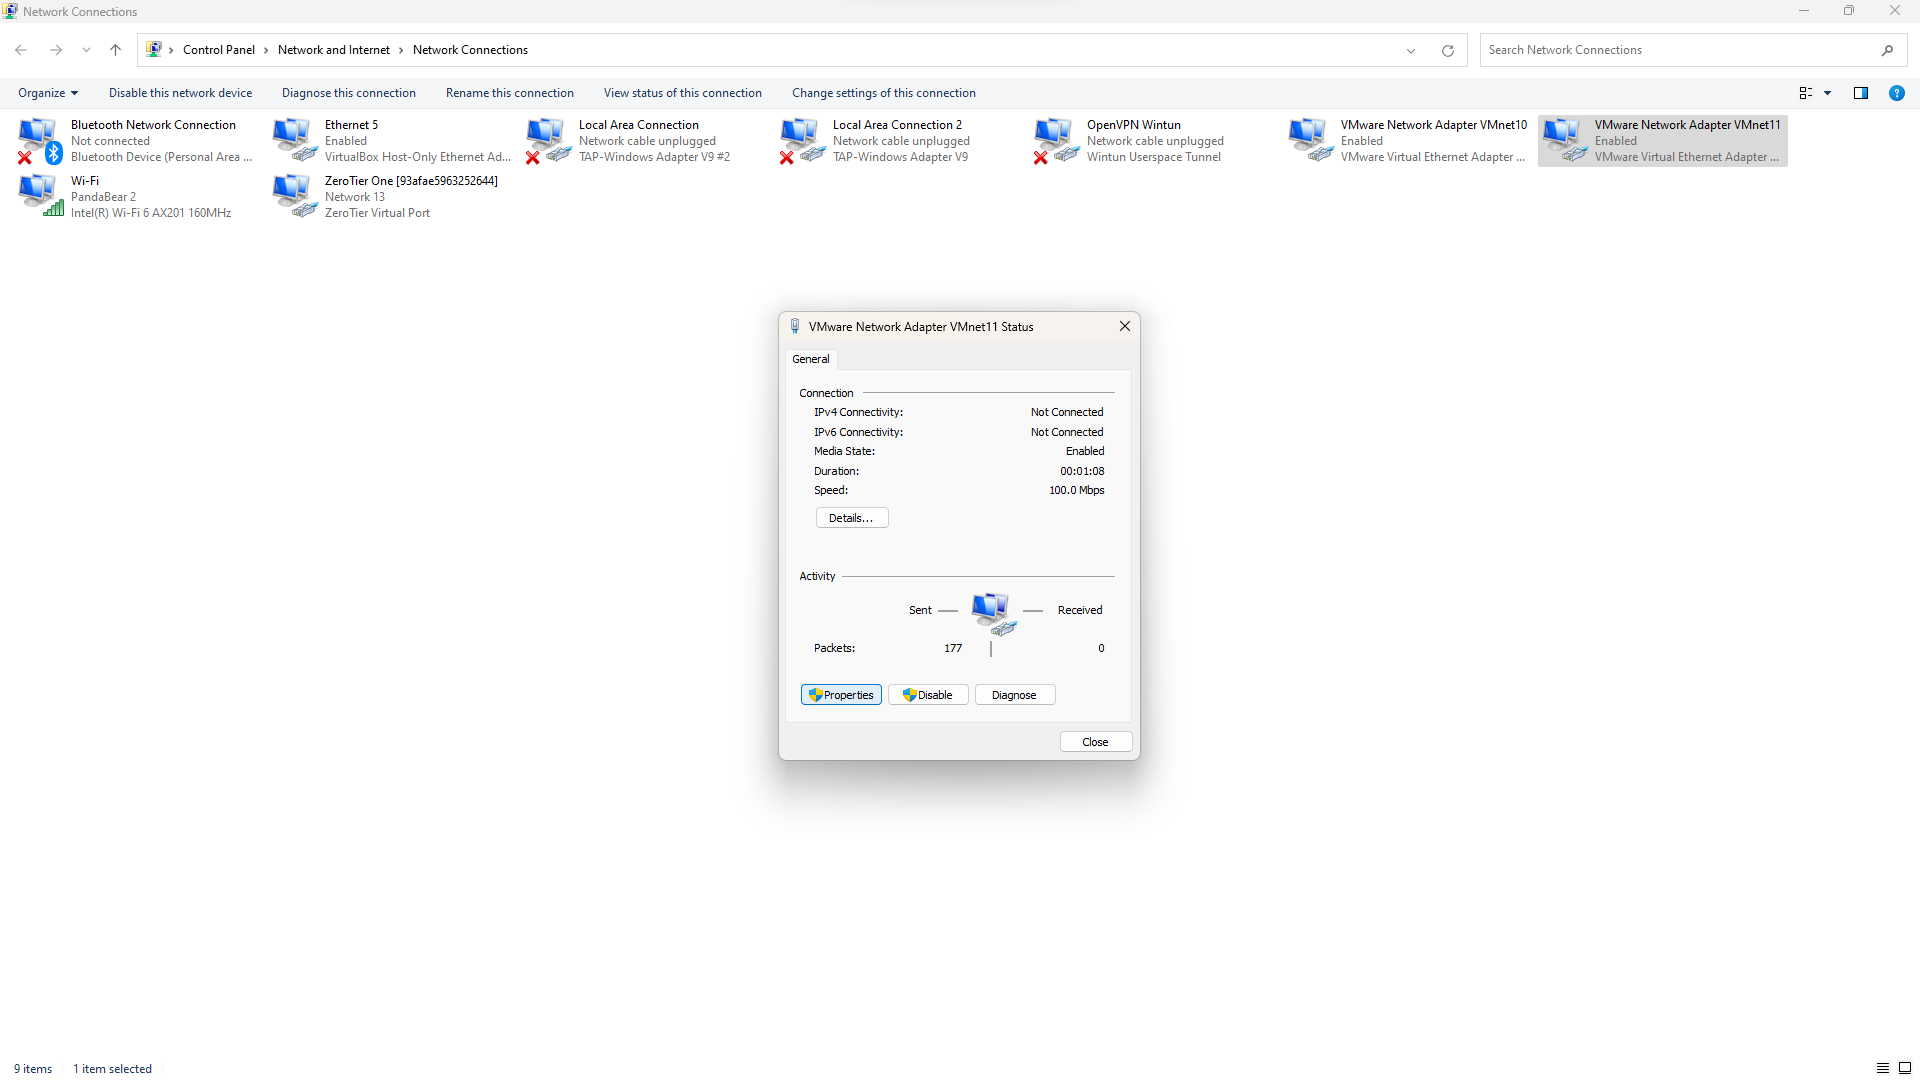
\includegraphics[width=0.85\textwidth]{06_00 (48)}
    \label{img:48}
    \caption{Параметры адаптера}
  \end{figure}
  
  Далее ищем пункт настроек \textit{IPv4} и открываем его:
  
  \begin{figure}[H]
    \centering
    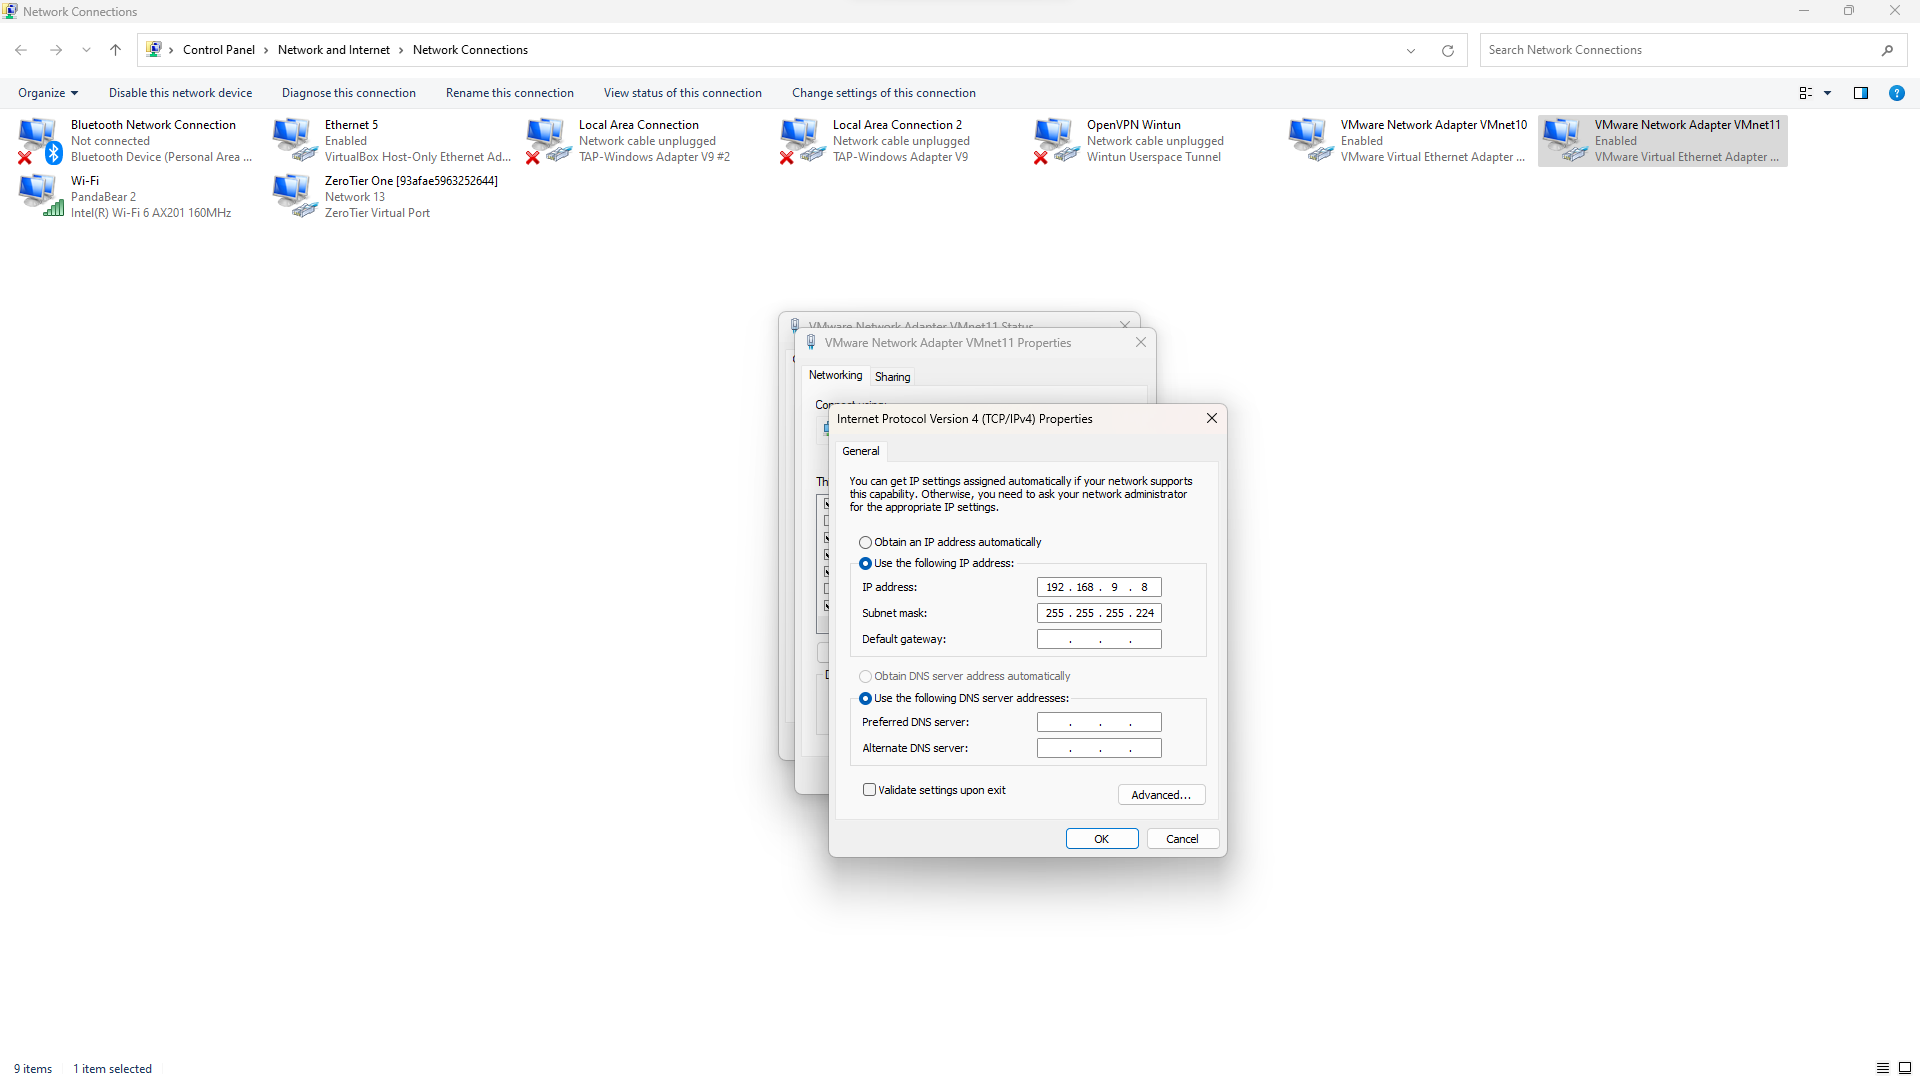
\includegraphics[width=0.85\textwidth]{06_00 (49)}
    \label{img:49}
    \caption{Указываем необходимые параметры}
  \end{figure}

  В пределах \textit{Host-Only} сети для хостовой машины был выбран адрес 192.168.9.8
  
  \subsubsection{Настройка второго адаптера в Linux}

  Открываем настройки виртуальной машины с linux:

  \begin{figure}[H]
    \centering
    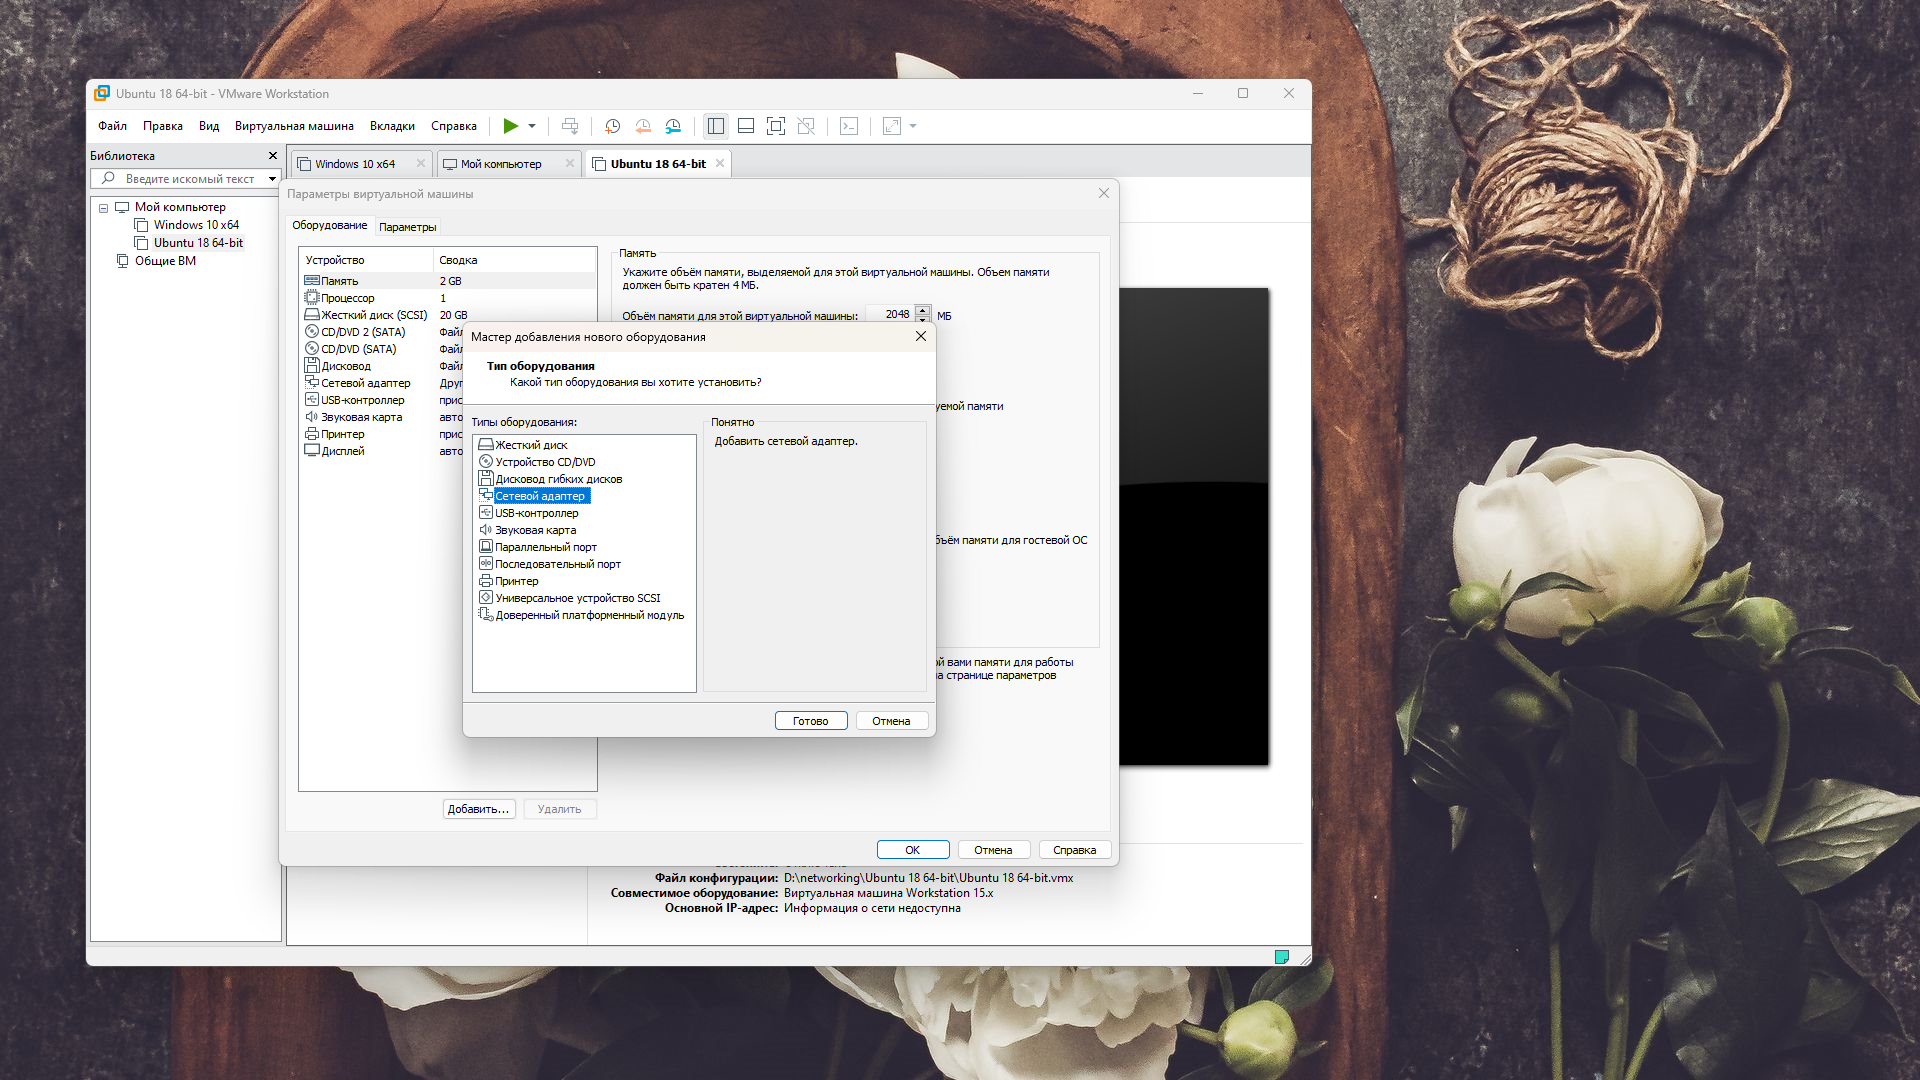
\includegraphics[width=0.85\textwidth]{06_00 (50)}
    \label{img:50}
    \caption{Создаем новый сетевой адаптер}
  \end{figure}
  
  \begin{figure}[H]
    \centering
    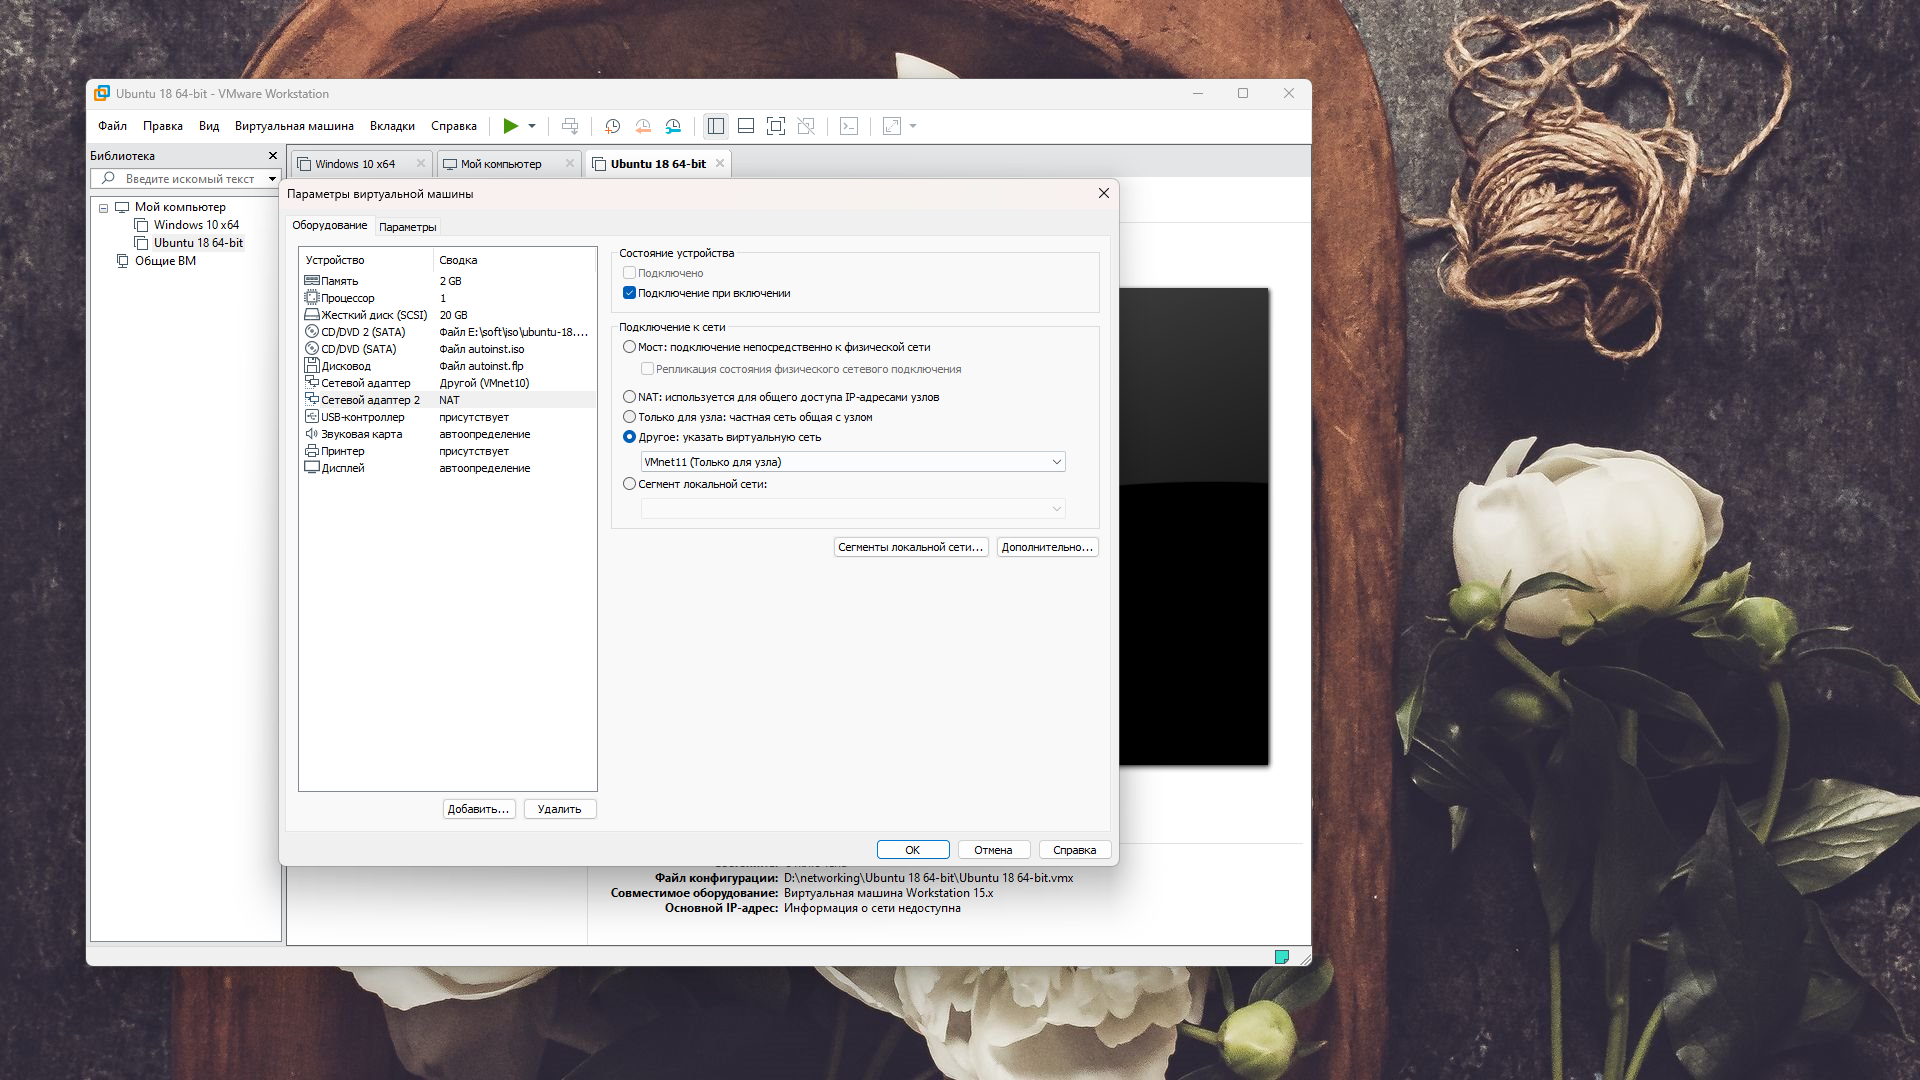
\includegraphics[width=0.85\textwidth]{06_00 (51)}
    \label{img:51}
    \caption{Подключаем его к \textit{Host-Only сети}}
  \end{figure}
  
  Перезагружаем машины и смотрим существующие сетевые интерфейсы:

  \begin{figure}[H]
    \centering
    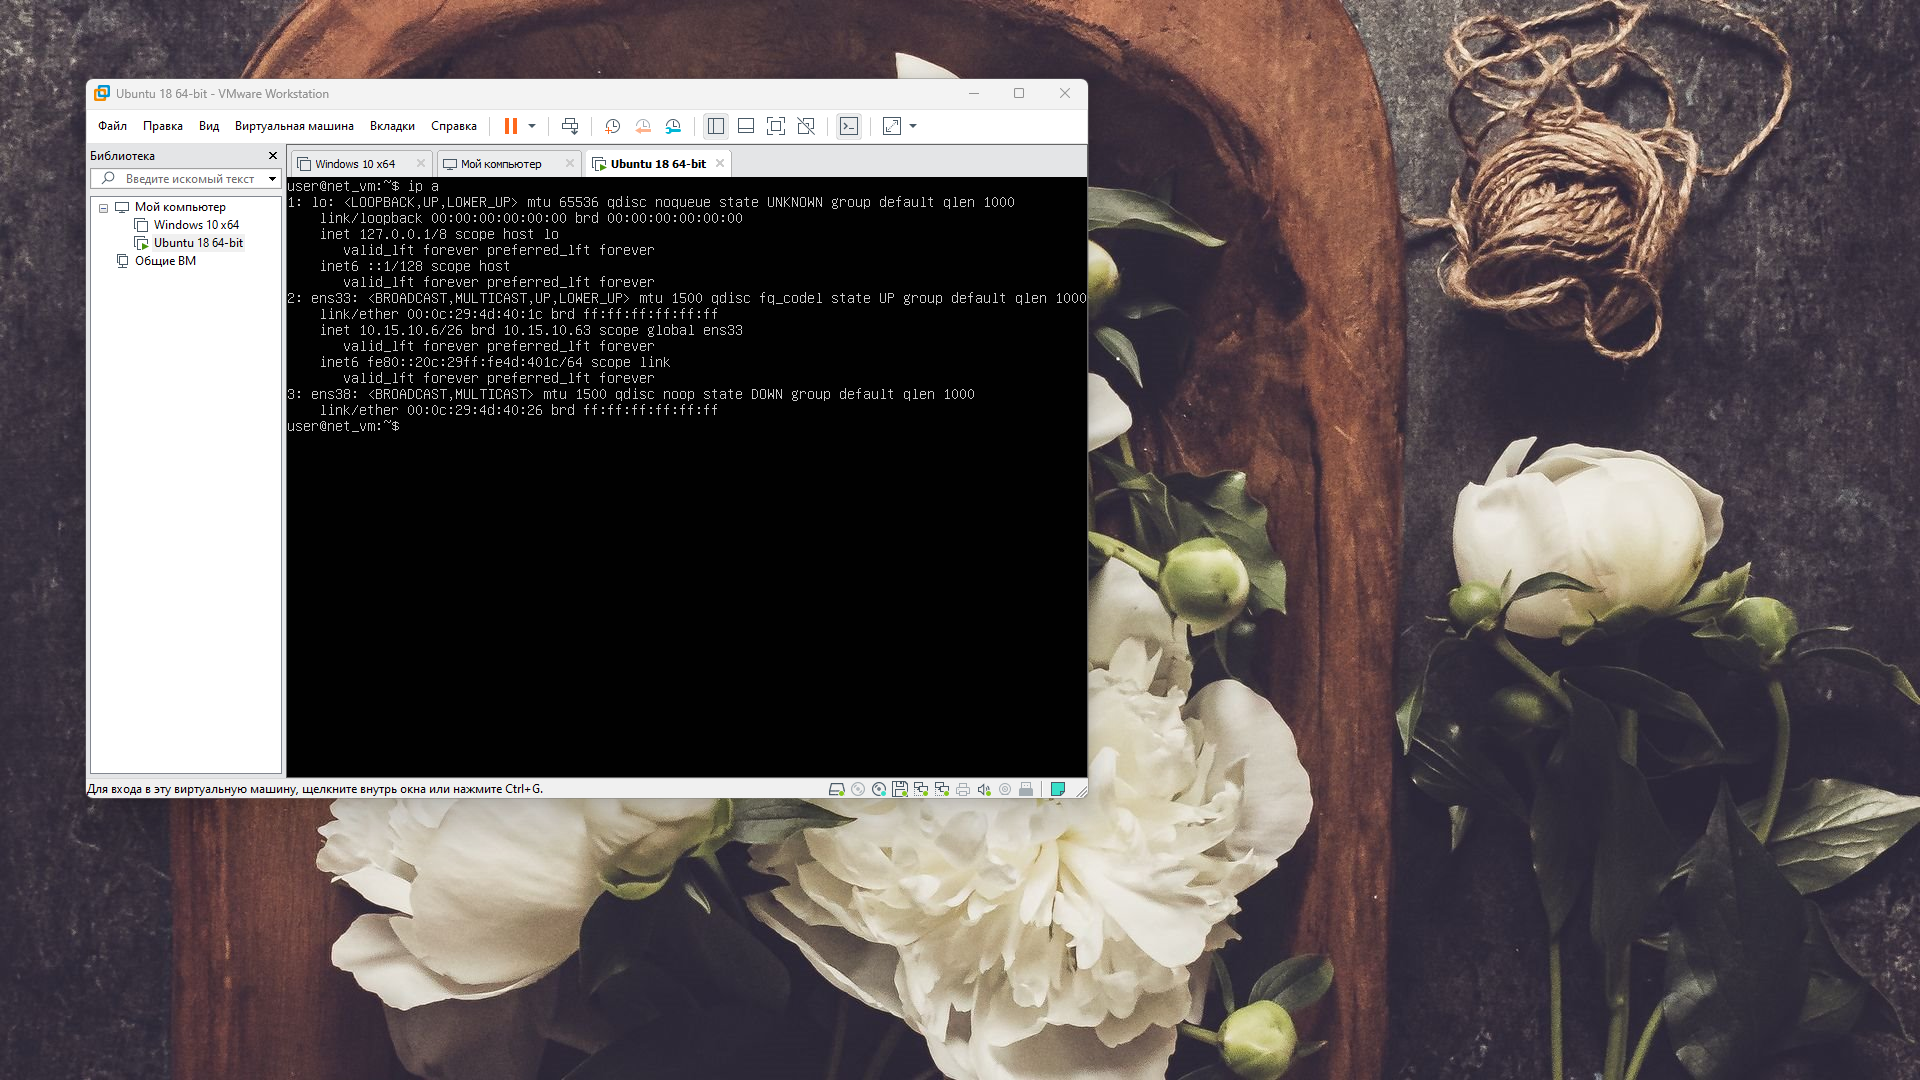
\includegraphics[width=0.85\textwidth]{06_00 (52)}
    \label{img:52}
    \caption{ip a - информация о сетевых интерфейсах}
  \end{figure}

  Появился новый - \textit{ens38}, через него происходит подключение к \textit{Host-Only} сети,
  настроим его:
  
  \begin{figure}[H]
    \centering
    \includegraphics[width=0.85\textwidth]{06_00 (53)}
    \label{img:53}
    \caption{Правки в конфигурационном файле}
  \end{figure}
  
  Для данного интерфейса также отключаем \textit{DHCP} и указываем \textit{IPv4} адрес 
  с постфиксом маски - 192.168.9.6/27.

  \begin{figure}[H]
    \centering
    \includegraphics[width=0.85\textwidth]{06_00 (54)}
    \label{img:54}
    \caption{Проверяем и применяем изменения - netplan generate и apply}
  \end{figure}
  
  Вступили ли изменения в силу можно проверить при помощи утилиты \textit{ip}:

  \begin{figure}[H]
    \centering
    \includegraphics[width=0.85\textwidth]{06_00 (55)}
    \label{img:55}
    \caption{ip a - информация о ens38}
  \end{figure}
  
  Видно, что \textit{IP} адрес и маска установлены корректно, теперь проверим, что виртуальная
  машина может подключиться к хостовой по ранее настроенному \textit{IP} адрес (из 192.168.9.6 в 192.168.9.8)
  при помощи \textit{ping}:
  
  \begin{figure}[H]
    \centering
    \includegraphics[width=0.85\textwidth]{06_00 (60)}
    \label{img:60}
    \caption{Проверка доступности}
  \end{figure}
  
  \subsubsection{Настройка \textit{Host-Only} сети в Windows}

  Подключим виртульную машину с Windows к той же сети:

  \begin{figure}[H]
    \centering
    \includegraphics[width=0.85\textwidth]{06_00 (61)}
    \label{img:61}
    \caption{Открываем настройки ВМ}
  \end{figure}
  
  \begin{figure}[H]
    \centering
    \includegraphics[width=0.85\textwidth]{06_00 (62)}
    \label{img:62}
    \caption{Добавляем новый сетевой адаптер}
  \end{figure}
  
  \begin{figure}[H]
    \centering
    \includegraphics[width=0.85\textwidth]{06_00 (63)}
    \label{img:63}
    \caption{Подключаем его к нужной сети}
  \end{figure}
  
  Включаем машину и переходим к настройке \textit{IP} адреса:

  \begin{figure}[H]
    \centering
    \includegraphics[width=0.85\textwidth]{06_00 (64)}
    \label{img:64}
    \caption{Открываем Панель Задач}
  \end{figure}
  
  \begin{figure}[H]
    \centering
    \includegraphics[width=0.85\textwidth]{06_00 (65)}
    \label{img:65}
    \caption{Пункт "Сеть и Интернет"}
  \end{figure}
  
  \begin{figure}[H]
    \centering
    \includegraphics[width=0.85\textwidth]{06_00 (66)}
    \label{img:66}
    \caption{Центр управления сетями и общим доступом}
  \end{figure}
  
  \begin{figure}[H]
    \centering
    \includegraphics[width=0.85\textwidth]{06_00 (67)}
    \label{img:67}
    \caption{Параметры нового сетевого интерфейса - Ethernet1}
  \end{figure}

  Указываем \textit{IP} адрес (был выбран 192.168.9.5) и маску подсети.
  
  \begin{figure}[H]
    \centering
    \includegraphics[width=0.85\textwidth]{06_00 (68)}
    \label{img:68}
    \caption{Проверка новых параметров}
  \end{figure}

  Новый адрес успешно присвоен, проверяем, что все машины видят новый узел сети:
  
  \begin{figure}[H]
    \centering
    \includegraphics[width=0.85\textwidth]{06_00 (69)}
    \label{img:69}
    \caption{Из виртуальной машины с Windows}
  \end{figure}
   
  \begin{figure}[H]
    \centering
    \includegraphics[width=0.85\textwidth]{06_00 (73)}
    \label{img:73}
    \caption{Из виртуальной машины с Linux}
  \end{figure}
  
  \begin{figure}[H]
    \centering
    \includegraphics[width=0.85\textwidth]{06_00 (74)}
    \label{img:74}
    \caption{С хостовой машины}
  \end{figure}
  
  \subsubsection{Создание образа Mikrotik OS}

  Тут уже будет производиться установка с iso образа:

  \begin{figure}[H]
    \centering
    \includegraphics[width=0.85\textwidth]{06_00 (75)}
    \label{img:75}
    \caption{Создаем новую ВМ}
  \end{figure}
  
  \begin{figure}[H]
    \centering
    \includegraphics[width=0.85\textwidth]{06_00 (76)}
    \label{img:76}
    \caption{Указываем тип конфигурации}
  \end{figure}
  
  \begin{figure}[H]
    \centering
    \includegraphics[width=0.85\textwidth]{06_00 (77)}
    \label{img:77}
    \caption{Устанавливаем путь до установочного iso образа}
  \end{figure}
  
  \begin{figure}[H]
    \centering
    \includegraphics[width=0.85\textwidth]{06_00 (78)}
    \label{img:78}
    \caption{Настраиваем имя ВМ}
  \end{figure}
  
  \begin{figure}[H]
    \centering
    \includegraphics[width=0.85\textwidth]{06_00 (79)}
    \label{img:79}
    \caption{Выделяем память для ВМ}
  \end{figure}
  
  \begin{figure}[H]
    \centering
    \includegraphics[width=0.85\textwidth]{06_00 (80)}
    \label{img:80}
    \caption{Производим настройку оборудования}
  \end{figure}
  
  Данную машину необходимо подклчючить к обеим ранее созданным сетям,
  поэтому потребуется создать два сетевых адаптера:

  \begin{figure}[H]
    \centering
    \includegraphics[width=0.85\textwidth]{06_00 (81)}
    \label{img:81}
    \caption{Сетевой адаптер для доступа к NAT сети}
  \end{figure}
  
  \begin{figure}[H]
    \centering
    \includegraphics[width=0.85\textwidth]{06_00 (83)}
    \label{img:83}
    \caption{Cетевой адаптер для доступа к \textit{Host-Only} сети}
  \end{figure}
  
  \begin{figure}[H]
    \centering
    \includegraphics[width=0.85\textwidth]{06_00 (84)}
    \label{img:84}
    \caption{Оборудование настроено}
  \end{figure}
  
  Далее производится установка ОС - указываем необходимые компоненты - system и dhcp, и нажимаем кнопку \textbf{i}:

  \begin{figure}[H]
    \centering
    \includegraphics[width=0.85\textwidth]{06_00 (85)}
    \label{img:85}
    \caption{Выбор компонентов}
  \end{figure}
  
  Дожидаемся установки и запуска системы, входим в учетную запись пользователя:
  
  \begin{figure}[H]
    \centering
    \includegraphics[width=0.85\textwidth]{06_00 (88)}
    \label{img:88}
    \caption{ВМ готова к работе}
  \end{figure}
  
  \subsubsection{Настройка NAT сети}

  \begin{figure}[H]
    \centering
    \includegraphics[width=0.85\textwidth]{06_00 (89)}
    \label{img:89}
    \caption{Получаем информацию о сетевых интерфейсах}
  \end{figure}

  Из них \textit{ether1} подключен к \textit{NAT} сети, а \textit{ethetr2} - к \textit{Host-Only}.
  
  \begin{figure}[H]
    \centering
    \includegraphics[width=0.85\textwidth]{06_00 (90)}
    \label{img:90}
    \caption{Устанавливаем IP адрес и маску подсети для каждого интерфейса}
  \end{figure}

  В \textit{NAT} сети данная машина будет иметь адрес 10.15.10.7, а в \textit{Host-Only} - 192.168.9.7 (семерки на конце).
  
  \begin{figure}[H]
    \centering
    \includegraphics[width=0.85\textwidth]{06_00 (91)}
    \label{img:91}
    \caption{Проверка применения настроек}
  \end{figure}

  Теперь проверим, что машина может ходить на шлюз по умолчанию в \textit{NAT} сети:
  
  \begin{figure}[H]
    \centering
    \includegraphics[width=0.85\textwidth]{06_00 (92)}
    \label{img:92}
    \caption{Пинг шлюза по умолчанию}
  \end{figure}
  
  Подключение к сети успешно, но нет маршрутизации в Интернет - настроим роутинг на 
  стандартный шлюз, которые уже имеет выход в глобальную сеть:

  \begin{figure}[H]
    \centering
    \includegraphics[width=0.85\textwidth]{06_00 (93)}
    \label{img:93}
    \caption{Роутинг на шлюз по умолчанию}
  \end{figure}

  Проверить наличие доступа в сеть можно отправкой пакетов на удаленный адрес, например на 8.8.8.8:
  
  \begin{figure}[H]
    \centering
    \includegraphics[width=0.85\textwidth]{06_00 (94)}
    \label{img:94}
    \caption{ping google dns}
  \end{figure}
  
  Осталось настроить DNS сервер:

  \begin{figure}[H]
    \centering
    \includegraphics[width=0.85\textwidth]{06_00 (95)}
    \label{img:95}
    \caption{Указываем DNS сервер и сразу проверяем на ya.ru}
  \end{figure}

  \subsection{Вторая часть}

  \textit{IP} адрес для \textit{Host-Only} сети уже настроен, проверим, что машина может
  производить подключение ко всем остальным участникам сети:
  
  \begin{figure}[H]
    \centering
    \includegraphics[width=0.85\textwidth]{06_00 (96)}
    \label{img:96}
    \caption{ping на хост, windows и linux виртуалки}
  \end{figure}
  
  \subsubsection{Настройка DHCP сервера}
  
  Выделим пул адресов, из которых наш сервер будет выбирать при назначении новому устройству:
  маска подсети имеет всего 5 единиц, что ограничевает сеть 30 устройствами, 4 из которых уже заняты.
  Чтобы точно попасть, укажем небольшой диапазон - от 192.168.9.10 до 192.168.9.15:
  
  \begin{figure}[H]
    \centering
    \includegraphics[width=0.85\textwidth]{06_00 (100)}
    \label{img:100}
    \caption{Создаем пул адресов}
  \end{figure}
  
  Теперь создаем сам сервер - указываем ему пул адресов, интерфейс для работы, имя, время жизни
  адреса, а также привязываем к сетевому интерфейсу:

  \begin{figure}[H]
    \centering
    \includegraphics[width=0.85\textwidth]{06_00 (101)}
    \label{img:101}
    \caption{Создаем DHCP сервер}
  \end{figure}
  
  Указываем шлюз, маску и адрес сети для этого сервера:

  \begin{figure}[H]
    \centering
    \includegraphics[width=0.85\textwidth]{06_00 (102)}
    \label{img:102}
    \caption{Настраиваем его параметры}
  \end{figure}

  Проверим работу нашего \textit{DHCP} сервера на машине с Linux:
  
  \begin{figure}[H]
    \centering
    \includegraphics[width=0.85\textwidth]{06_00 (103)}
    \label{img:103}
    \caption{Что было ДО}
  \end{figure}

  Включаем \textit{DHCP} клиент на интерфейсе \textit{ens38}:
  
  \begin{figure}[H]
    \centering
    \includegraphics[width=0.85\textwidth]{06_00 (104)}
    \label{img:104}
    \caption{Новая конфигурация}
  \end{figure}
  
  \begin{figure}[H]
    \centering
    \includegraphics[width=0.85\textwidth]{06_00 (105)}
    \label{img:105}
    \caption{Проверяем и применяем изменения}
  \end{figure}
  
  \begin{figure}[H]
    \centering
    \includegraphics[width=0.85\textwidth]{06_00 (106)}
    \label{img:106}
    \caption{Смотрим новый IP адрес}
  \end{figure}

  Как видно, \textit{DHCP} сервер действительно выдал ВМ адрес из указанного пула,
  значит все работает верно (192.168.9.15).
  
  Посмотрим таблицу \textit{DHCP} сервера:

  \begin{figure}[H]
    \centering
    \includegraphics[width=0.85\textwidth]{06_00 (107)}
    \label{img:107}
    \caption{Выданные IP адреса}
  \end{figure}
  
  \begin{figure}[H]
    \centering
    \includegraphics[width=0.85\textwidth]{06_00 (108)}
    \label{img:108}
    \caption{Сделаем существующее присовение адреса 192.168.9.15 к машине с Linux статическим - DHCP сервер всегда будет выдавать ей этот адрес}
  \end{figure}
  
  Далее сделаем так, чтобы машине с Windows тоже всегда выдавался один и тот же адрес,
  но этот адрес мы зададим сами. Для этого нужен \textit{MAC} сетевого адаптера на 
  ВМ с \textit{Windows}:

  \begin{figure}[H]
    \centering
    \includegraphics[width=0.85\textwidth]{06_00 (109)}
    \label{img:109}
    \caption{Получаем MAC адрес}
  \end{figure}
  
  \begin{figure}[H]
    \centering
    \includegraphics[width=0.85\textwidth]{06_00 (110)}
    \label{img:110}
    \caption{Присваиваем этому MAC адресу фиксированный IP адрес}
  \end{figure}
  
  \begin{figure}[H]
    \centering
    \includegraphics[width=0.85\textwidth]{06_00 (111)}
    \label{img:111}
    \caption{Включаем DHCP для сетевого адаптера в ВМ с Windows}
  \end{figure}
  
  \begin{figure}[H]
    \centering
    \includegraphics[width=0.85\textwidth]{06_00 (112)}
    \label{img:112}
    \caption{Проверяем изменения}
  \end{figure}
  
  Машине действительно был выдан необходимый \textit{IP} адрес.

  Также, есть графический интерфейс, доступ к которому есть со всех машин, включая хостовую:

  \begin{figure}[H]
    \centering
    \includegraphics[width=0.85\textwidth]{06_00 (1)}
    \label{img:113}
    \caption{UI для настройки Mikrotik}
  \end{figure}


  \section{Вывод}

  В ходе данной лабораторной работы я научился создавать и конфигурировать сетевые адаптеры
  в VM Ware, назначать IP адреса, включать и отключать DHCP клиент, а также настраивать собственный
  DHCP сервер.

\end{document}
